\documentclass[fontsize=11pt, % size of the font
			   paper=a4,
			   chapterprefix=true,
			   WordMark=atelier/logo/FAU-NatFak.pdf,
			   ExtraLogo=atelier/logo/DepMathLogo.pdf,
			   % oneside, % other option: oneside
			   % chapterprefix=false, % specifies if the word chapter is printed for chapter headings
			   % BCOR=0mm, % offset for binding
			   setPDF, % sets twosided=semi, BCOR=0, 
			   %DIV=calc, % if not specified
			   % showframe, % show the page layout
			   bibstyle=styleB,
			   ]{fau-book}
% #####################################################################
% ########################################################################################
% Font encoding and font specification
% ----------------------------------------------------------------------------------------
\usepackage[T1]{fontenc}
\usepackage{lmodern}
% ########################################################################################
% The following specifies the titlepage and can not be deleted
% ----------------------------------------------------------------------------------------
\title{Consistency, Robustness and Sparsity for Learning Algorithms}
\subtitle{Konsistenz, Robustheit und Dünnbesetztheit von Lern-Algorithmen}
\author{Tim Roith}
\thesistype{}
\degree{Dr. rer. nat.}
\degprog{Mathematik}% specify the degree program
\Referee{first=Martin Burger}% Referees
\Advisor{first=M.Sc. C}
%\renewcommand{\supervisors}{Hello :)} % use this to specify the supervisor area yourself
%\subdate{Today} % Use this if you want to specify the date on the titlepage
% ########################################################################################
\keywords{topicA, topicB, topicC} %keywords of your thesis
\setpdfinfo % For additional information in the pdf file
% ########################################################################################
% Bibliography
% ----------------------------------------------------------------------------------------
\addbibresource{backmatter/thesis-bibliography.bib}
% ########################################################################################
% Load the fau style packages with customization
% ----------------------------------------------------------------------------------------
% Color themes
\usepackage[NatClassic]{styles/fau-colors}

% Appearence of boxes and page
\usepackage[thmboxing=styleC,
			boxingstyle=styleC,
			chapterheader=styleC, 
			footerheader=styleA,
			%noabbrev % no abbreviations in cleveref
			]{styles/fau-appearence}
% Command spec for symbols
\usepackage{styles/fau-symbols}
% ########################################################################################
% ########################################################################################
% ########################################################################################
% Custom commands and additional packages
% Put additional command definition below.
% Load additional packages below 
% ----------------------------------------------------------------------------------------
%
\usepackage{kantlipsum}
\usepackage[totoc]{idxlayout}
\usepackage[final]{pdfpages}
\usepackage{subcaption}
\usetikzlibrary{positioning}
\usetikzlibrary{shapes.multipart}
\usepackage{wrapfig}

\makeatletter
\renewcommand{\maketitle}{
\begin{titlepage}
\thispagestyle{empty}
\begin{center}
\vspace*{1cm}
\huge \textbf{\@title} \\[5mm]
\large \@subtitle\\
\vspace{2cm}
\LARGE\textbf{\@thesistype}\\[5mm]
\Large zur Erlangung des Doktorgrades\\[5mm]
\textbf{\@degree \\[5mm]
im Studiengang
\@degprog\\[5mm]
}
am Department Mathematik der\\ Friedrich-Alexander-Universit\"at
Erlangen-N\"urnberg\\[1cm]
vorgelegt am \textbf{\@subdate} \\[3mm]
von \textbf{\@author}
\vfill
\normalsize
\supervisors
\end{center}
%
% \begin{minipage}{0.5\textwidth}
% %\vspace*{10mm}
% \includegraphics[width=\textwidth]{\WordMark}
% \end{minipage}
% \hfill
% \begin{minipage}{0.4\textwidth}
% \includegraphics[width=\textwidth]{\ExtraLogo} \vspace{3mm}
% \end{minipage}
\end{titlepage}
}
\makeatother

\newcommand\expprefix{}
\let\latexorigthechapter\thechapter
\renewcommand{\thechapter}{\expprefix\latexorigthechapter}


\usepackage{todonotes}
\usepackage{csquotes}

%---------------
% colors
\definecolor{sky}{rgb}{0.51, 0.79, 0.99}
\definecolor{apple}{rgb}{0.43, 0.8, 0.24}
\definecolor{grape}{rgb}{0.99, 0.35, 0.34}
\definecolor{orong}{rgb}{1.0, 0.55, 0.0}

\newcommand{\bc}{\color{black}}

%
% ..............................................................................
% Set colors for hypersetup
% ------------------------------------------------------------------------------
%
\hypersetup{
		breaklinks=true,
		urlcolor=BaseColor,
		citecolor=grape,
		linkcolor=BaseColor}

\acknowledgementtext{%
The three years of my PhD have been a thrilling period of learning, both in terms of scientific knowledge and personal growth. This journey allowed me to explore exciting research directions, travel to various parts of the world, and, most significantly, meet a lot of people. I want to thank all of my colleagues at FAU Erlangen-Nürnberg for making the experience at the Chair of Applied Mathematics what it was. I especially want to express my gratitude to the following people:
%
\begin{itemize}
\item Martin Burger for granting me a student assistant position back in 2018, even though I hail from the Upper Palatinate. Since then, I have relished the unique blend of freedom to express myself, coupled with dependable support whenever required.
%
\item Daniel Tenbrinck for being the heart of our former chair at FAU, serving as the driving force behind every important social event, being an inherently helpful person, setting up the GPU servers, and, most importantly, for winning the Best Teaching Award in 2021 and giving me credit for it. During my time at FAU, we worked a lot together, especially on teaching-related topics, which always turned out to be a great success. I miss the idea of preparing lectures together. I hope we can collaborate in the future, and I am sure we'll see each other whenever time allows.
%
\item Leon Bungert for basically co-supervising my PhD and for teaching me a lot about mathematics, culture, cooking, and colorful shirts. Given the wealth of experiences we've shared during the last four years, it's not easy to express all of this within a few lines. Apart from our collaborations on an academic level, I want to thank you for being a very close friend.
%
\item Antonio Esposito for being a really nice guy, greatly improving my fake Italian accent, and, most of all, for being part of our group. I was really sad when you left for Oxford, and I hope to meet you again soon.
%
\item Alex Rossi for sparking my interest in patches, teaching me how to dress austere and introducing me to authentic Italian desserts. I think you're a great guy, and I've always loved hanging out with you.
%
\item Lukas Weigand for introducing me to the green book, helping with the exercise sheets for numerics, and teaching me a lot about gradient flows. I look forward to working together with you in the future.
%
\item Lorenz Kuger for sharing the office with me for a long time, despite being the best-organized PhD student I know, not getting too annoyed about every non-work related activity I started in the office, and for being a great colleague. Transitioning to Hamburg was especially easy thanks to your pioneering a lot of bureaucratic ground.
%
\item All the other colleagues I spent time with in Erlangen, or met around the world, namely:
\begin{itemize}
\item Philipp Wacker for making me aware of the field of statistics,
\item Jannik Hausladen for helping me a lot with our MRI project,
\item Alexander Prechtl for always bringing the servers back to life (together with Daniel), when I crashed them,
\item Jeff Calder for collaborating with Leon and me on Lipschitz leaning and writing that very nice graph learning package, which made everything a lot easier,
\item Nicolás García Trillos for organizing a nice mini-symposium together with me in Tokyo,
\item and Konstantin Riedl for being yet another great mathematician from the Upper Palatinate.
\end{itemize}
%
\item All my other colleagues and short-time office mates that just recently joined the Burger group, with whom I am now starting a new chapter in Hamburg.
%
\item Astrid Bigott for always being understanding of my difficult relationship with bureaucracy and for finding all the mistakes I ever made in any kind of form.
%
\item My proofreaders Leon, Norman, Martin, and Samira.
%
\item My parents for always showing me affection and supporting me unconditionally. Although I am not always physically there, I will never lose my connection to home. Also, I want to extend my thanks to Miezer for always letting me use his pictures for imaging purposes.
%
%
%
%
%
%
\item Samira Kabri for teaching me about FNOs. 
\end{itemize}
}
\usepackage{tikz}
\usetikzlibrary{shapes.arrows, fadings}
\definecolor{fourierblue}{rgb}{0.78, 0.84, 0.93}
\usetikzlibrary{arrows}
\usetikzlibrary{calc,arrows.meta,fadings}
%
\RedeclareSectionCommand[
tocnumwidth=2em
]{chapter}
\RedeclareSectionCommand[
tocindent=2em,
tocnumwidth=2.8em
]{section}
\RedeclareSectionCommand[
tocindent=4.8em,
tocnumwidth=4em
]{subsection}
\hypersetup{hypertexnames=false}



\begin{document}
%-------------------------------------------------
\frontmatter
%-------------------------------------------------
\maketitle
\printacknowledgement
\tableofcontents
\listoffigures
\printnomenclature
%-------------------------------------------------
% ======================================
\chapter{Inhalt und Struktur}
%

Diese Arbeit ist in zwei Hauptteile strukturiert, \cref{part:Intro}, welche die Themen und Resultate der Publikation präsentiert und erklärt, welche in \cref{part:Prints} erneut abgedruckt sind.

%
%
\begin{center}%
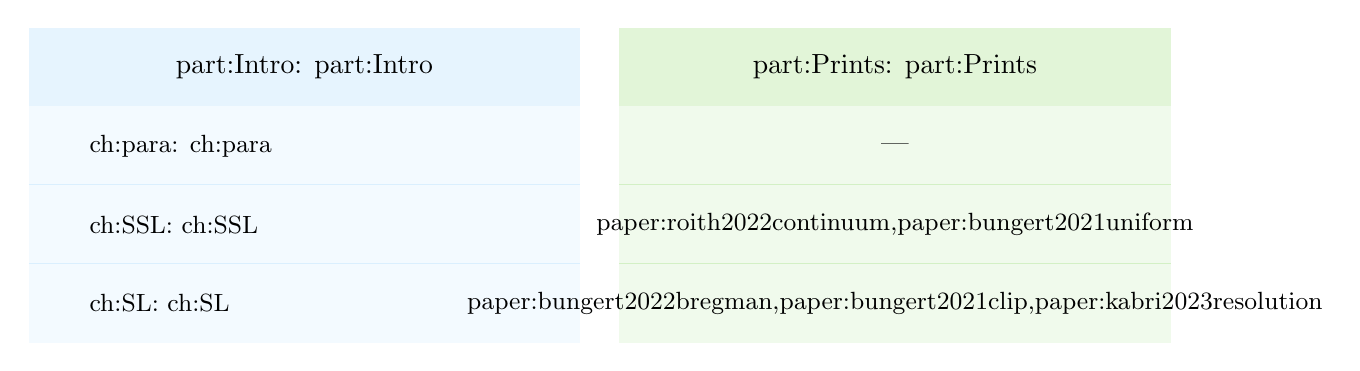
\begin{tikzpicture}
\hypersetup{linkcolor=black}%
\filldraw[fill=sky!20, draw=none] (0,11) rectangle (7.,10); %
\node[draw=none, align=center] at (3.5,10.5) {\cref{part:Intro}: \nameref{part:Intro}};
%
\filldraw[fill=sky!10, draw=none] (0,10) rectangle (7,9); %
\node[draw=none, align=center] at (3.5,9.5) {%
\parbox{.45\textwidth}{\small\cref{ch:para}: \nameref{ch:para}}};
%
\draw[draw=sky!30, thick] (0,9) -- (7, 9); %
%
\filldraw[fill=sky!10, draw=none] (0,9) rectangle (7,8); %
\node[draw=none, align=center] at (3.5,8.5) {%
\parbox{.45\textwidth}{\small\cref{ch:SSL}: \nameref{ch:SSL}}};
%
\draw[draw=sky!30, thick] (0,8) -- (7, 8); %
%
\filldraw[fill=sky!10, draw=none] (0,8) rectangle (7,7); %
\node[draw=none, align=center] at (3.5,7.5) {%
\parbox{.45\textwidth}{\small\cref{ch:SL}: \nameref{ch:SL}}};
%
%
%
\filldraw[fill=apple!20, draw=none] (7.5,11) rectangle (14.5,10);%
\node[draw=none, align=center] at (11.,10.5) {\cref{part:Prints}: \nameref{part:Prints}};
%
\filldraw[fill=apple!10, draw=none] (7.5,10) rectangle (14.5,9); %
\node[draw=none, align=center] at (11.,9.5) {---% 
};
%
\draw[draw=apple!30, thick] (7.5,9) -- (14.5, 9); %
%
\filldraw[fill=apple!10, draw=none] (7.5,9) rectangle (14.5,8); %
\node[draw=none, align=center] at (11.,8.5) {%
{\small\cref{paper:roith2022continuum,paper:bungert2021uniform}}};
%
\draw[draw=apple!30, thick] (7.5,8) -- (14.5, 8); %
%
\filldraw[fill=apple!10, draw=none] (7.5,8) rectangle (14.5,7); %
\node[draw=none, align=center] at (11.,7.5) {%
{\small\cref{paper:bungert2022bregman,paper:bungert2021clip,paper:kabri2023resolution}}};
\end{tikzpicture}
\end{center}
%
%
%
%
\section*{Einleitung und Motivation}
%
%
Das Gebiet des maschinellen Lernens entstand in den 1950er Jahren, motiviert durch die Idee, einen Computer Algorithmen und Muster entdecken zu lassen, ohne sie explizit von Hand anordnen zu müssen. Nach der Anfangsphase und mehreren \enquote{AI-winters} \cite{steele1996evolution} haben zahlreiche wichtige Entwicklungen -- z.~B. die Wiederentdeckung der \enquote{Backpropagation}, welche ursprünglich auf \cite{kelley1960gradient,rosenblatt1962principles} zurückgeht und dann in \cite{rumelhart1986learning} popularisiert wurde, siehe z.~B. \cite{schmidhuber2022annotated} -- zur Relevanz der Lernmethoden beigetragen. Die Fortschritte im Bereich von Computer-Hardware, zusammen mit der Verfügbarkeit großer Datenmengen, haben schließlich den Enthusiasmus für maschinelles Lernen der letzten Jahre entfacht. Während \enquote{deep} Learning Methoden, d.~h. Techniken, die mehrere neuronale Layer verwenden, wie sie ursprünglich in \cite{rosenblatt1958perceptron} vorgeschlagen wurden, die prominentesten Beispiele sind, gibt es eine ganze Familie von lernbasierten Strategien, welche aktiv in Bereichen wie Computer Vision \cite{chai2021deep}, Sprachverarbeitung \cite{khurana2023natural} oder für medizinische Zwecke \cite{shehab2022machine} angewendet werden. In dieser Arbeit konzentrieren wir uns hauptsächlich auf datenbasierte Ansätze, angewendet auf Klassifizierungsaufgaben, wobei die konkrete Modalität der gegebenen Daten unsere Strategie bestimmt. Wir konzentrieren uns auf überwachtes Lernen -- der Datensatz besteht nur aus Eingabe-Ausgabe-Paaren, d.~h., er ist vollständig gelabelt -- und halb-überwachtes Lernen -- die Daten sind nur teilweise gelabelt.

Beide datenbasierten Methoden waren vor allem in den letzten 20 Jahren sehr erfolgreich. Allerdings weisen die manchmal rein heuristischen Lernstrategien auch gravierende Nachteile auf. Beim überwachten Lernen ist man oft an der Generalisierung eines Klassifizierers interessiert, d.~h. wie akkurat ist das Ergebnis auf ungesehenen Eingaben, die nicht Teil der Trainingsdaten sind. In \cite{goodfellow2014explaining} wurde entdeckt, dass die Ausgaben des Klassifizierers durch kleine, scheinbar unsichtbare Störungen, die als \textit{adversarial attacks} bekannt sind, vollständig verfälscht werden können. Allgemeiner führt uns dieses Phänomen zum Thema \textit{Robustheit} unter Eingabestörungen. Nehmen wir an, dass ein Mensch und eine Maschine eine Eingabe $\inp$ als vom Typ $c$ einstufen würden. In einer eher vagen, aber anschaulichen Formulierung lautet die wichtigste Implikation, die wir für eine Eingabe $\inpp$ erhalten wollen
%
\begin{align*}
\left.
\begin{gathered}
\inpp\text{ liegt nahe an }\inp,\\
\inpp\text{ wird von einem Menschen noch als }c\text{ eingestuft}
\end{gathered}
\right\}
\Rightarrow
\text{die Maschine stuft }\inpp\text{ als }c  \text{ ein.} 
\end{align*}
%
Neben adversarial Examples gehört dazu auch das Ändern der Auflösung von Bildern, welche die Klassifizierung durch einen Menschen nicht verändern, sofern sie hinreichend klein sind. In jedem Fall zeigt das Vorhandensein dieser Störungen kritische Schwächen der Lernmethoden auf und erfordert ein besseres theoretisches Verständnis der verwendeten Modelle. An dieser Stelle wird die mathematische Grundlage des Fachgebiets relevanter und es kommen Eigenschaften ins Spiel, die über die Klassifizierungsleistung hinausgehen und die in dieser Arbeit diskutiert werden.

Im halb-überwachten Setting betrachten wir Graphbasierte Algorithmen, wie sie ursprünglich in \cite{zhu2003semi} mit dem Graph Laplace vorgeschlagen wurden. Das Hauptproblem, das wir in dieser Arbeit hervorheben, wurde zuerst in \cite{nadler2009statistical} beobachtet, nämlich dass die Klassifizierungsleistung mit steigender Dimension der Daten deutlich abnimmt. Es stellte sich heraus, dass die mit dem Graph-Laplace erhaltenen Lösungen über den gesamten Datensatz hinweg konstant sind, wenn die Dimension größer als zwei ist, was mit dem Sobolev Einbettungssatz \cite{adams2003sobolev} in Verbindung gebracht werden kann. Dieses Problem zeigt sich vor allem, wenn die Zahl der unbeschrifteten Datenpunkte gegen unendlich geht, was uns zu der Frage der \textit{Konsistenz} für halb-überwachte Algorithmen führt.

Ein Problem, das für überwachte und halb-überwachte Algorithmen gleichermaßen gilt, ist der hohe Bedarf an Rechenressourcen. Das Training eines neuronalen Netzes erfordert in der Regel den Einsatz von GPUs über einen langen Zeitraum. Dies macht den Prozess einerseits für weniger leistungsfähige Maschinen oder sogar mobile Geräte undurchführbar und erzeugt andererseits große Mengen an CO$_2$-Emissionen \cite{hoefler2021sparsity}. Für graphbasiertes, halb-überwachtes Lernen müssen zunächst Entfernungen zwischen vielen Datenpunkten berechnet werden, um Kantengewichte zu erhalten, was eine kostspielige Aufgabe ist. Außerdem skaliert die Rechenkomplexität verschiedener Probleme auf einem gegebenen Graphen mit der Anzahl der Kanten. Beispielsweise skaliert die Laufzeit von Dijkstras Algorithmus zur Berechnung kürzester Pfade in einem Graphen bereits linear mit der Anzahl der Kanten. In dieser Arbeit ist das Schlüsselwort zur Reduzierung der Rechenlast in beiden Fällen \textit{Dünnbesetztheit}. Das Konzept von dünnbesetzten Matrizen ist tief in der numerischen linearen Algebra verwurzelt \cite{lanczos1952solution,golub2013matrix} und besteht im Wesentlichen darin, Nullen in einer Matrix auszunutzen, um die Berechnungszeit zu beschleunigen. Bei neuronalen Netzen kann dies dadurch erreicht werden, dass die Gewichtsmatrizen der Layer dünnbesetzt sein müssen. Bei Graphen bedeutet eine dünnbesetzte Konnektivitätsmatrix einfach, dass nur eine kleine Anzahl an Kanten aktiv ist, was ebenfalls die Rechenkosten reduziert.
%
%
\paragraph{Beiträge in dieser Arbeit}
%
Anknüpfend an die zuvor genannten Themen befasst sich diese Arbeit mit \textit{Konsistenz, Robustheit} und \textit{Dünnbesetztheit} von überwachten und halb-überwachten Lernalgorithmen. 


Für letztere betrachten wir hauptsächlich das sogenannte Lipschitz-Learning \cite{nadler2009statistical}, für die wir Konvergenz und Konvergenzraten für diskrete Lösungen zu Lösungen im Kontinuum zeigen, wenn die Anzahl der Datenpunkte gegen unendlich geht. Dabei arbeiten wir mit Annahmen, welche sehr dünnbesetzte und daher rechnerisch attraktive Graphen zulässt.


Bei überwachtem Lernen befassen wir uns mit der Robustheit gegen adversarial Attacks und Auflösungsänderungen. Im ersten Fall schlagen wir einen effizienten Algorithmus vor, der die Lipschitz-Konstante \cite{lipschitz1877lehrbuch} eines neuronalen Netzes bestraft und ein damit robustes Netz trainiert. Im Multiresolution-Setting analysieren wir die Rolle von neuronalen Fourier-Operatoren, wie sie in \cite{li2020fourier} vorgeschlagen wurden, und ihre Verbindung zu normalen Faltungsoperatoren \cite{fukushima1980neocognitron}. Im Hinblick auf die Rechenkomplexität des Trainings neuronaler Netze schlagen wir einen auf Bregman Iterationen basierenden Algorithmus \cite{osher2005iterative} vor, der dünnbesetzte Gewichtsmatrizen während des gesamten Trainings ermöglicht. Zusätzliche analysieren wir die Konvergenz der stochastische Adaption der ursprünglichen Bregman Iterationen.


\paragraph{Struktur der Exposition} In \cref{ch:para} stellen wir die Lernparadigmen und Grundbegriffe vor, die in dieser Arbeit verwendet werden. Anschließend stellen wir in \cref{ch:SSL} die Themen zur Konsistenz beim halb-überwachten Lernen auf Graphen vor. Nach einer erläuternden Einführung heben wir die Hauptbeiträge von \cite{roith2022continuum,bungert2021uniform} hervor. Dabei versuchen wir Redundanz zu den Publikationen in \cref{part:Prints} zu vermeiden und dennoch einen verständlichen Kontext zu ermöglichen. In \cref{ch:SL} kommentieren wir die Themen zum überwachten Lernen. Nach einer zusätzlichen Einleitung enthält das Kapitel drei Abschnitte, in denen die Arbeiten \cite{kabri2023resolution,bungert2021clip,bungert2022bregman} einzeln vorgestellt werden. Schließlich werden in \cref{ch:C} die Inhalte der gesamten Arbeit zusammengefasst und mögliche zukünftige Richtungen aufgezeigt.
%
%
%
%
%
\section*{Publikationen und Beitragsauflistung}
Die folgenden Arbeiten sind Teil dieser Dissertation und werden in \cref{part:Prints} erneut abgedruckt.

\printbibliography[keyword={papersA}, resetnumbers=true, heading=none]
\printbibliography[keyword={papersB}, resetnumbers=true, heading=none]

\noindent%
Die folgenden Preprints sind kein Teil dieser Arbeit, geben aber zusätzliche Einsichten in die behandelten Themen.

\printbibliography[keyword={papersC}, resetnumbers=true, heading=none]

Im Folgenden führen wir TRs Beiträge zu den oben genannten Publikationen auf. 

\paragraph{\cite{roith2022continuum}:} Diese Arbeit baut auf den Erkenntnissen von TRs Masterarbeit auf. Es ist allerdings wichtig anzumerken, dass die Resultate signifikant erweitert wurden und konzeptionell stärker als die der Masterarbeit sind, siehe dazu Abschnitt 3.3 in der Dissertation. TR adaptierte die Kontinuum-Limit-Theorie für den $L^\infty$-Fall, erarbeitet die meisten Beweise und schrieb einen großen Teil des Papers. In Zusammenarbeit mit LB, identifizierte er entscheidende Gebiets-Annahmen, welche es erlauben auch mit nicht-konvexen Gebieten zu arbeiten und bewies Konvergenz für angenäherte Randbedingungen.

\paragraph{\cite{bungert2021uniform}:} In Zusammenarbeit mit LB, arbeitete TR an den Konvergenzbeweisen, basierenden auf den Ideen von JC. Zusammen mit LB und JC bewies er das Hauptresultat und die verschiedenen Lemmata, die darauf hinführen. Hierbei beschäftigte er sich vor allem mit der Adaption der Theorie für AMLEs auf den Graph-Fall, was das entscheidende Element für die ganze Arbeit ist. Weiterhin, trug er zur Gestaltung und Implementierung der numerischen Experimente, die im Paper durchgeführt wurden bei. 

\paragraph{\cite{bungert2021clip}:} TR erarbeitete den Algorithmus, der im Paper vorgeschlagen wird, zusammen mit LB, basierend auf dessen Idee. Zusammen mit LS, RR und DT führte er die numerischen Beispiele durch und schrieb große Teile des Quellcodes. Weiterhin schrieb er entscheidende Teile des Papers, wobei DT das Dokument Korrektur lies und klarer formulierte.

\paragraph{\cite{bungert2022bregman}:} TR erweiterte LBs Idee, Bregman Iterationen für dünnbesetztes Training einzusetzen, konzipiert durch DT. Zusammen mit MB und LB erarbeitete er die Konvergenzbeweise der stochastischen Bregman Iteration. Hier schlug er auch eine fundierte Initialisierungsstrategie vor. Weiterhin führte er die numerischen Beispiele durch und schrieb den größten Teil des Quellcodes.

\paragraph{\cite{kabri2023resolution}:} Diese Arbeit beruht auf SKs Masterarbeit und verwendet die ursprünglichen Ideen MBs, zu Auflösungsinvarianz mithilfe von FNOs. Im Paper erarbeitete TR die Beweise zur Wohldefiniertheit und Fréchet-Differenzierbarkeit, zusammen mit SK. Er schrieb große Teile des Papers und des Source-Codes, wobei DT bei der Korrektur der publizierten Version mitgeholfen hat. Hierbei führte er die numerischen Studien zusammen mit SK durch.


% ========================================================================================
\chapter{Preface}\label{ch:preface}

This work is structured into two main parts, \cref{part:Intro} the presentation and explanation of the topics and results presented in \cref{part:Prints}, the peer-reviewed articles. 
%
%
\begin{center}%
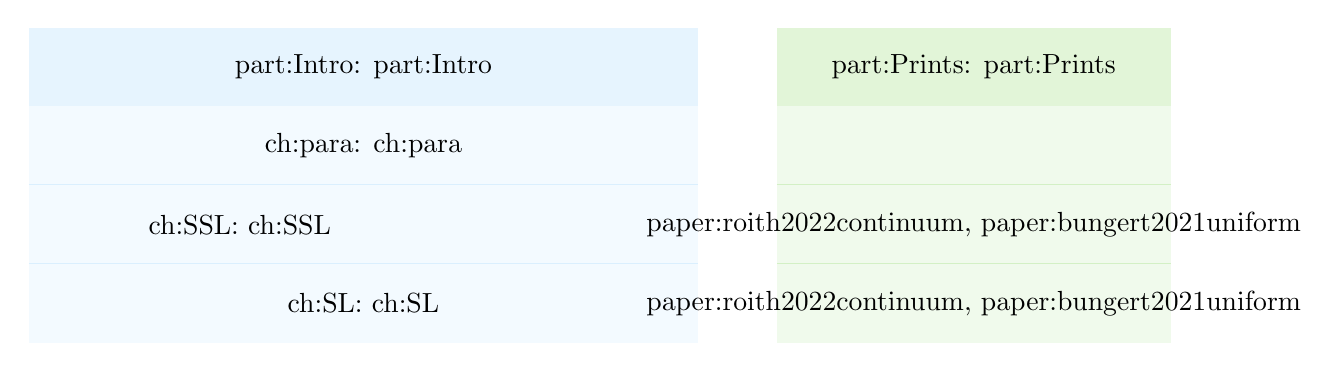
\begin{tikzpicture}
\hypersetup{linkcolor=black}%
\filldraw[fill=sky!20, draw=none] (0,11) rectangle (8.5,10); %
\node[draw=none, align=center] at (4.25,10.5) {\cref{part:Intro}: \nameref{part:Intro}};
%
\filldraw[fill=sky!10, draw=none] (0,10) rectangle (8.5,9); %
\node[draw=none, align=center] at (4.25,9.5) {%
\cref{ch:para}: \nameref{ch:para}};
%
\draw[draw=sky!30, thick] (0,9) -- (8.5, 9); %
%
\filldraw[fill=sky!10, draw=none] (0,9) rectangle (8.5,8); %
\node[draw=none, align=center] at (4.25,8.5) {%
\parbox{.45\textwidth}{\cref{ch:SSL}: \nameref{ch:SSL}}};
%
\draw[draw=sky!30, thick] (0,8) -- (8.5, 8); %
%
\filldraw[fill=sky!10, draw=none] (0,8) rectangle (8.5,7); %
\node[draw=none, align=center] at (4.25,7.5) {%
\cref{ch:SL}: \nameref{ch:SL}};
%
%
%
\filldraw[fill=apple!20, draw=none] (9.5,11) rectangle (14.5,10);%
\node[draw=none, align=center] at (12.,10.5) {\cref{part:Prints}: \nameref{part:Prints}};
%
\filldraw[fill=apple!10, draw=none] (9.5,10) rectangle (14.5,9); %
\node[draw=none, align=center] at (12.,9.5) {% 
};
%
\draw[draw=apple!30, thick] (9.5,9) -- (14.5, 9); %
%
\filldraw[fill=apple!10, draw=none] (9.5,9) rectangle (14.5,8); %
\node[draw=none, align=center] at (12.,8.5) {%
\cref{paper:roith2022continuum, paper:bungert2021uniform}};
%
\draw[draw=apple!30, thick] (9.5,8) -- (14.5, 8); %
%
\filldraw[fill=apple!10, draw=none] (9.5,8) rectangle (14.5,7); %
\node[draw=none, align=center] at (12.,7.5) {%
\cref{paper:roith2022continuum, paper:bungert2021uniform}};
\end{tikzpicture}
\end{center}
%
%
\cref{part:Intro} consists of three chapters, of which the first explains the paradigms, \emph{unsupervised}, \emph{semi-supervised} and \emph{supervised} learning. The other chapters are the split up thematically, concerning the topics semi-supervised and supervised learning respectively. In each of these chapters a short introduction provides the necessary framework allowing us to explain the main contributions. The following publications are reprinted in \cref{part:Prints}:


\printbibliography[keyword={papersA}, resetnumbers=true, heading=none]
\printbibliography[keyword={papersB}, resetnumbers=true, heading=none]

The following two works that are not part of this thesis but provide an additional insight.

\printbibliography[keyword={papersC}, resetnumbers=true, heading=none]

\subsection*{TR's Contribution}

Here we list TR's contribution to the publications included in the thesis.

\paragraph{\cite{roith2022continuum}:} This work builds upon the findings in TR's master thesis \cite{roith2022msc}. It is however important to note that the results constitute a significant extension and are conceptually stronger than the ones in \cite{roith2022msc}, see \cref{sec:GConv}. TR adapted the continuum limit framework to the $L^\infty$ case, worked out most of the proofs and wrote a significant part of the paper. In collaboration with LB, he identified the crucial domain assumptions that allow to work on non-convex domains and proved convergence for approximate boundary conditions.

\paragraph{\cite{bungert2021uniform}:} In collaboration with LB, TR worked on the convergence proofs building upon the ideas of JC. He contributed to both the numeric and the analysis conducted in the paper.

\paragraph{\cite{bungert2021clip}:} TR worked out the main algorithm proposed in the paper together with LB, based on LB's idea. Together with LS and RR he conducted the numerical examples and also wrote most of the source code. Furthermore, he wrote large parts of the paper.

\paragraph{\cite{bungert2022bregman}:} TR expanded LB's ideas of employing Bregman iteration for sparse training. Together with MB and LB he worked out the convergence analysis of stochastic Bregman iterations. Here, he also proposed a profound sparse initialization strategy. Furthermore, he conducted the numerical examples and wrote most of the source code.

\paragraph{\cite{kabri2023resolution}:} This work is based on SK's masters thesis, employing the initial ideas of MB for resolution invariance with FNOs. In the paper TR worked out the proofs for well-definedness and Fréchet-differentiability, together with SK. He wrote large parts of the paper and the source code. Here, he conducted the numerical studies in collaboration with SK.


%-------------------------------------------------
\mainmatter
%-------------------------------------------------
\part{Exposition}\label{part:Intro}
\chapter{Introduction}
%
%
The field of \textit{machine learning} emerged in the 1950s \cite{samuel1959some, rosenblatt1958perceptron}, motivated by the idea of letting a machine discover algorithms and patterns without having to explicitly arrange them by hand. After the initial phase and multiple \enquote{AI-winters} \cite{steele1996evolution}, numerous important developments---e.g. the rediscovery of the backpropagation algorithm, originally due to \cite{kelley1960gradient,rosenblatt1962principles} and then popularized in \cite{rumelhart1986learning}, see e.g. \cite{schmidhuber2022annotated}---contributed to the relevance of learning methods. The advances in computer hardware together with the availability of large amounts of data, finally allowed the machine learning enthusiasm of the recent years to spark. While \enquote{deep} learning methods---i.e. techniques involving many stacked neural layers as originally proposed in \cite{rosenblatt1958perceptron}---are the most prominent examples, there is a whole zoo of learning-based strategies that are actively applied in fields like computer vision \cite{chai2021deep}, natural language processing \cite{khurana2023natural} or healthcare \cite{shehab2022machine}. In this work we mainly focus on data-driven approaches, applied to classification tasks, where the concrete modality of the given data determines our approach. Namely, we focus on supervised---the dataset consists of input-output pairs, i.e. is fully labeled---and the semi-supervised---the data is only partially labeled---learning tasks.

For both regimes especially the last 20 years have seen great success of these data-driven methods. However, the sometimes purely heuristic learning strategies also exhibit serious drawbacks. In the supervised setting one is usually interested in the generalization behavior of a learned classifier, i.e. how good is the performance on unseen inputs that are not part of the given training data. Unfortunately in \cite{goodfellow2014explaining} it was discovered, that this performance can be completely corrupted, by small, seemingly invisible perturbations known as \textit{adversarial attacks}. More generally this phenomenon leads us to the issue of \textit{input robustness}. Given some input $\inp$ and suppose that a human and some machine would classify this input to be of type $c$. In a rather vague but demonstrative formulation the key implication for transformed input $\inpp$ we want to obtain is
%
\begin{align*}
\left.
\begin{gathered}
\inpp\text{ is close to }\inp,\\
\inpp\text{ is still classified as }c\text{ by a human}
\end{gathered}
\right\}
\Rightarrow
\text{the machine classifies }\inpp\text{ as } c. 
\end{align*}
%
Next to adversarial examples this also includes resolution changes of images, which do not---if they are reasonably small---change the classification by a human. For the semi-supervised setting \todo{weiter schreiben}
\chapter{Learning Paradigms}\label{ch:para}

Throughout this thesis, we assume to be given data $\Inp_n\subset\Inp\subset \R^d$ consisting of $n$ data points. We consider the task of \emph{learning} a function $f:\tilde{\Inp}\to \Oup$ from the given data, where $\Oup$ denotes the output space. In our case the set $\tilde{\Inp}\subset\Inp$ is usually chosen either as the set of data points $\Inp_n$ or as the whole space $\Inp$. The two most important cases for us are listed below.
%
\begin{itemize}
\item \textbf{Classification}: The function $\net$ assigns a label to each $x\in \tilde\Inp$ out of $C\in\N$ possible classes, i.e. $\Oup=\{1,\ldots,C\}$. In some architectures the last layer of the neural network is given as a vector $\oup\in\R^C$. Typically, this vector is a probability vector, i.e. 
%
\begin{align*}
y\in \Delta^C := \left\{z\in[0,1]^C: \sum_{i=1}^C z_i = 1\right\}.
\end{align*}
%
This can be enforced via the softmax function \cite{bridle1990probabilistic} $\operatorname{soft max}:\R^C\to\R^C$
%
\begin{align*}
\operatorname{soft max}(z)_i := \frac{\exp(z_i)}{\sum_{j=1}^C \exp(z_j)} 	
\end{align*}
%
which was actually introduced by Boltzman in \cite{boltzmann1868studien}. This allows the interpretation that the $i$th entry of $\net_\param(\inp)\in\Delta^C$ models the probability that $\inp$ belongs to class $i$. In order to obtain a label one can simply choose the maximum entry, i.e.  $\argmax_{i=1,\ldots,C} \net_\param(\inp)_i$.
%
\item \textbf{Image denoising}: The function $\net$ outputs a denoised version of an input image. Here we have $\Inp = \Oup=\R^{K\times N\times M}$, where
%
\begin{itemize}
\item $K\in\N$ is the number of color channels,
\item $N,M$ denote the width and height of the image.
\end{itemize}
\end{itemize}
%
The learning paradigms we consider in this thesis, differ by their usage of labeled data. We review the concepts in the following.
%
\clearpage%
\section{Unsupervised Learning}
\begin{wrapfigure}{r}{.5\textwidth}
\centering
\includegraphics[width=.5\textwidth]{atelier/paradigms/UL.pdf}
\end{wrapfigure}

In the case of unsupervised learning we are not given any labeled data. In our context the most important application is data clustering. Other tasks involve dimensionality reduction or density estimation, see \cite{subramanya2014graph}. The clustering task consists of grouping data based on some similarity criterion. In this sense, clustering can also be interpreted as classification, i.e., the desired function is a mapping $\net:\tilde{\Inp}\to \{1,\ldots, C\}$ where $C\in\N$ denotes the number of clusters. Typically, one wants to obtain a clustering of the given data set, i.e., $\tilde\Inp = \Inp_n$. We list some of the typical clustering methods below:
%
\begin{itemize}
\item K-means algorithm \cite{steinhaus1956division},
\item expectation maximization  \cite{dempster1977maximum},
\item Cheeger cuts \cite{GarcSlep15, szlam2009total, trillos2016consistency, garcia2022graph},
\item spectral clustering \cite{trillos2018variational, trillos2021geometric, hoffmann2022spectral}.
\end{itemize}
%
%
Unsupervised learning is not the main focus of this present work. However, we note that especially the concepts developed in \cite{GarcSlep15} for Cheeger cuts are crucial for the continuum limit framework in \cref{sec:GConv}.

\section{Supervised Learning}\label{sec:PSL}
\begin{wrapfigure}{r}{.5\textwidth}
\centering
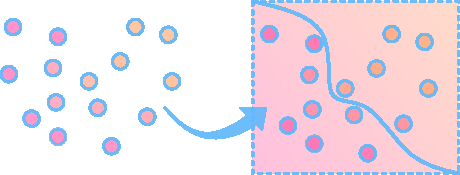
\includegraphics[width=.5\textwidth]{atelier/paradigms/SL.pdf}
\end{wrapfigure}
%
In this setting, each data point $x\in\Inp_n$ is labeled, via a given function $g:\Inp_n\to\Oup$ such that we have a finite training set $\mathcal{T} = \{(x,g(x)): x\in\Inp_n\}$. The task is to infer a function defined on the underlying space, $\net:\Inp \to\Oup$, i.e., we want to assign a label to unseen inputs $x\in\Inp$ that are not necessarily part of the given data. Often, one models the problem via a joint probability function $P_{\Inp,\Oup}$ and assumes that the training data are independent and identically distributed (i.i.d) with respect to $P_{\Inp,\Oup}$. In this interpretation, the aim is to approximate the conditional $P_{\Inp,\Oup}(y|x)$ for an input $\inp\in\Inp$ and output $\oup\in\Oup$. 

In order to \emph{learn} the function $\net$ from the given data, one needs to choose a parameterized class of functions, where typically each element can be describe by a finite number of parameters. Among others, common methods or parametrizations include
%
\begin{itemize}
\item support vector machines \cite{cortes1995support, scholkopf2005support},
\item decision trees \cite{morgan1963problems, Brei},
\item neural networks \cite{Turing,rosenblatt1958perceptron, minsky1969introduction}.
\end{itemize}
%
We refer to \cite{SCHMIDHUBER201585} for an exhaustive historical overview.

In \cref{ch:SL} we exclusively focus on supervised learning algorithms employing neural networks, where the concrete setting is given at the start of the chapter.
%
%
%
\section{Semi-Supervised Learning}\label{sec:PSSL}
\begin{wrapfigure}{r}{.5\textwidth}
\centering
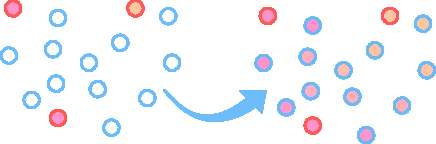
\includegraphics[width=.5\textwidth]{atelier/paradigms/SSL.pdf}
\end{wrapfigure}
%
In the semi-supervised setting we assume that only a fraction of the data $\Inp_n$ is labeled, i.e., we are given a a function $g:\conset_n\to\Oup$ where $\conset_n\subset\Inp_n$ is the non-empty set of labeled data. Typically this constitutes only a small fraction of all available points, i.e. $\abs{\conset_n}<<\abs{\Inp_n}$. In this thesis we restrict ourselves to the \emph{transductive setting}, i.e. we want to infer a function acting only on the data $\net: \Inp_n\to \Oup$. This is opposed to the inductive setting, where $\net$ also classifies unseen points $x\in\Inp$, \cite{zhu2005semi}. Common algorithms and methods include
%
\begin{itemize}
\item expectation maximization and mixture models \cite{dempster1977maximum,cozman2003semi},
\item self-training and co-training \cite{blum1998combining},
\item graph-based learning \cite{zhu2005semi}.
\end{itemize}
%
%
Mostly, we consider the extension task with $\Oup$ being chosen as $\R$. In application this can be seen as a binary classification task, where for $o\in\conset_n$ we have $g(o)=1$ if $o$ belongs to a some class and $g(o)=0$ otherwise. The function $f:\Inp_n\to\R$ then determines the probability that any vertex $x\in \Inp_n$ belongs to this class, where we can binarize the output via some thresholding, e.g.,
%
\begin{align*}
x \text{ belongs to the class } \Leftrightarrow f(x) > 1/2.	
\end{align*}
%
This methodology can be extended to classification tasks beyond the binary case, via the so-called one-vs-all technique \cite{zhu2003semi}. Given a classification problem with $C\in\N$ possible classes, we assume that the labeling function $g:\conset_n\to \Delta^C$ outputs one-hot vectors, i.e. $g(o)_c =1$ if $o$ belongs to class $c$ and $g(o)_c=0$ otherwise, for every $c = 1,\ldots, C$. We then perform the binary classification problem \enquote{$x$ belongs to class $c$} for every $c=1,\ldots,C$, by considering the extension task of 
%
\begin{align*}
g_c:\conset_n\to\R\qquad g_c(o) = g(o)_c,
\end{align*}
%
which yield functions $f_c:\Inp_n\to[0,1],c=1,\ldots,C$. The final output can then either obtained by emplyoing a Bayes classifier \cite{devroye2013probabilistic}, i.e. $f:\Inp_n\to\{1,\ldots, C\}$ 
%
\begin{align*}
f(x) := \argmax_{c=1,\ldots, C} f_c(x)
\end{align*}
%
or by applying a softmax to obtain a probability vector, i.e. $f:\Inp_n\to\Delta^C$ 
%
\begin{align*}
f(x) := \operatorname{soft max}\left(f_1(x), \ldots, f_c(x)\right).
\end{align*}
%
In \cref{ch:SSL} we focus on graph-based learning algorithms, however we refer to \cite{zhu2005semi} for an overview of semi-supervised learning algorithms. 

\chapter{Consistent Semi-Supervised Learning on Sparse Graphs}\label{ch:SSL}

This chapter considers the consistency of graph-based semi-supervised learning methods and contextualizes the topics provided in the prints \cite{roith2022continuum, bungert2021uniform, bungert2022ratio}. We are given partially labeled data, where the task is to obtain a labeling on the  whole graph. Here, we consider learning algorithms on graphs and are especially interested in the following aspects:
%
\begin{itemize}
\item \textbf{Consistency:} what is the behavior in the infinite data limit?
\item \textbf{Sparsity:} how does sparsity of the graph weights affect this behavior?
\end{itemize}
%
%
In \cite{roith2022continuum} we first consider $\Gamma$-convergence of discrete $L^\infty$ functionals to their continuum counterpart. This allows to then show convergence of minimizers and therefore consistency. The proofs allow for very sparse graphs, however they only directly apply to the Lipschitz extension task, which does not allow for unique solutions. We refer to \cref{sec:GConv} for more details.

The issue of non-uniqueness is addressed in \cite{bungert2021uniform}, which considers uniform convergence of graph infinity harmonic functions to their continuum counterpart. These functions are in fact special solutions of the extension task  in \cite{roith2022continuum}, namely so-called absolutely minimizing Lipschitz extensions, which are---under certain assumptions---unique. Again, we are able to work with a very mild scaling assumption that allows for sparse graphs. Furthermore, we are able to prove the first quantitative convergence rates, where we provide the key insight, that a rate for graph distance functions transfers to a rate for infinity harmonic functions. The main contributions are presented in \cref{sec:RatConv}.

To allow even sparser graphs, directly at the connectivity threshold, we consider first passage percolation in \cite{bungert2022ratio}. Here, we prove a ratio convergence of a graph distance function on a Poisson point cloud. The results can ultimately be employed to show convergence rates for Lipschitz learning. Details are provided in \cref{sec:Perc}.

Before we present these works we first introduce the setting of consistency for graph-based SSL in \cref{sec:GSSL}. We then discuss the $p$-Laplacian in \cref{sec:pLap} both in the continuum and the graph setting. Similarly, we then introduce the problem we are actually concerned namely the $\infty$-Laplacian and Lipschitz extensions in \cref{sec:LipExt}. With the necessary tools and background we are then able to present the main contributions on consistency of Lipschitz learning in the infinite data limit.
%
%
%
\begin{center}%
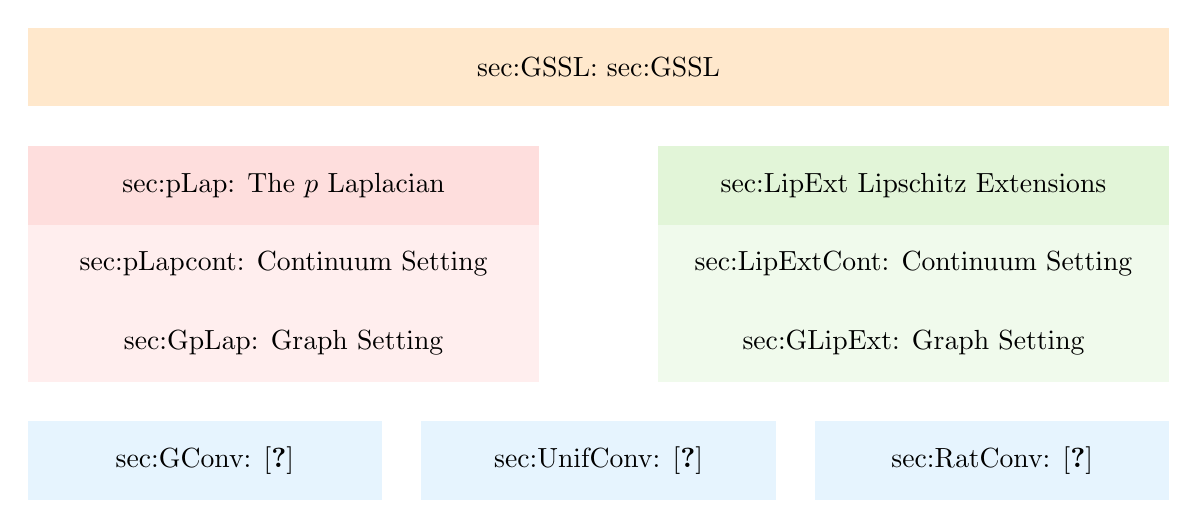
\begin{tikzpicture}
%
\hypersetup{linkcolor=black}%
\filldraw[fill=orong!20, draw=none] (0,12.5) rectangle (14.5,11.5) node[midway] {%
\cref{sec:GSSL}: \nameref{sec:GSSL}};
\filldraw[fill=grape!20, draw=none] (0,11) rectangle (6.5,10) node[midway] {\cref{sec:pLap}: The $p$ Laplacian}; %
\filldraw[fill=grape!10, draw=none] (0,10) rectangle (6.5,9) node[midway] {\cref{sec:pLapcont}: Continuum Setting};
\filldraw[fill=grape!10, draw=none] (0,9) rectangle (6.5,8) node[midway] {\cref{sec:GpLap}: Graph Setting};
%
%
%
%
%
\filldraw[fill=apple!20, draw=none] (8,11) rectangle (14.5,10) 
node[midway] {\cref{sec:LipExt} Lipschitz Extensions}; %
\filldraw[fill=apple!10, draw=none] (8,10) rectangle (14.5,9) 
node[midway] {\cref{sec:LipExtCont}: Continuum Setting}; %
\filldraw[fill=apple!10, draw=none] (8,9) rectangle (14.5,8) 
node[midway] {\cref{sec:GLipExt}: Graph Setting}; %
%
%
%
%
\filldraw[fill=sky!20, draw=none] (0,7.5) rectangle (4.5, 6.5) node[midway] {%
\cref{sec:GConv}:  \cite{roith2022continuum}};
%
\filldraw[fill=sky!20, draw=none] (5,7.5) rectangle (9.5, 6.5) node[midway] {%
\cref{sec:UnifConv}:  \cite{bungert2021uniform}};
%
\filldraw[fill=sky!20, draw=none] (10,7.5) rectangle (14.5, 6.5) node[midway] {%
\cref{sec:RatConv}:  \cite{bungert2022ratio}};
\end{tikzpicture}
\end{center}
%
%
%
%
%
%
%
\section{Graph-based SSL and Consistency}\label{sec:GSSL}

\begin{wrapfigure}{r}{.5\textwidth}
\centering
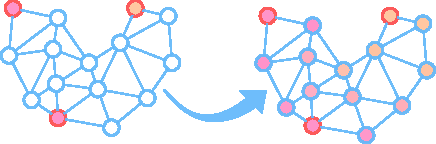
\includegraphics[width=.5\textwidth]{atelier/paradigms/GSSL.pdf}
\end{wrapfigure}

In the semi-supervised learning setting of \cref{sec:PSSL}, we are given a finite set $\domain_n\subset \tilde{\domain}$ consisting of $n$ points, where $\tilde{\domain}$ 
denotes the input space. We assume that a non-empty subset $\conset_n \subset \domain_n$ is labeled, i.e., we are given a labeling function
$\vec g:\conset_n\to\R$. From now on we denote functions acting on a discrete set $\domain_n$ using bold symbols to distinguish them from functions acting on the continuum $\tilde\domain$. In particular, the space of functions on $\domain_n$ can simply be identified with $\R^n$, since $\{\vec u:\domain_n\to\R\} \sim \R^n.$
%
\noindent%
The semi-supervised learning problem consists in finding an extension of $\vec g$ from $\conset_n$ to the whole set $\domain_n$, i.e.
%
\begin{gather}\label{eq:SSL}
\begin{gathered}\tag{SSL}
\text{find } \vec u:\domain_n\to\R,\\
\text{such that } \vec u(x) = \vec g(x) \text{ for all } x\in\conset_n.
\end{gathered}
\end{gather}
%
%
%
%
In order to obtain meaningful solutions, one usually incorporates the \emph{smoothness assumption} \cite{subramanya2014graph} which can be informally stated as follows:
%
\begin{center}
\enquote{\textit{Points that are close together are more likely to share a similar label.}}
\end{center}
%
%

\begin{remark}{Notational Remark}{}
In \cref{ch:para} we employ the symbol $\Inp$ to denote the input set, which is now replaced by $\domain$. This due to the fact, that the prints \cite{bungert2021uniform, bungert2022ratio, roith2022continuum} employ this notation for which we choose to use it here.
\end{remark}
%
%
Often one assumes that the points $x\in\domain_n$ are i.i.d. w.r.t. a distribution $\mu$ with density $\rho:\domain\to\R$. However, as observed in \cite{roith2022msc}, the data distribution is not directly relevant for the works in \cite{roith2022continuum, bungert2021uniform}. Therefore, we can usually work with more general sets $\domain_n$.
%
%
\subsection{Weighted Graphs}
In order to employ the smoothness assumption we need a notion of \enquote{closeness} on the set $\domain_n$, for which we introduce weighted graphs. Namely we define a weighting function $w$ that allows to compare points in $\domain_n$ and therefore induces the desired notion. 
%
\begin{definition}{Weighted Graphs}{}
For a finite set $\domain_n$ and a weight function $w_n:\domain_n\times \domain_n\to\R$, the tuple $(\domain_n,w_n)$ is called a \emph{weighted graph}.
\end{definition}
%
%
\paragraph{Other Notions of Graphs}
Typically, a graph is defined as a pair $(\domain_n,E)$ where $E$ denotes the set of edges. Here, 
one has two cases:
\begin{itemize}
\item \emph{Undirected graph:} $E=\{ \{x,y\}: \text{there is an edge between } x\in \domain_n \text{ and } y\in \domain_n\}$, i.e., s
$E\subset 2^{\domain_n}$ and each edge is undirected, since $\{x,y\}=\{y,x\}$.
%
\item \emph{Directed graph:} $E=\{ (x,y): \text{there is an edge from } x \text{ to } y\}$, i.e.,
$E\subset \domain_n\times \domain_n$ and each edge is directed and $(x,y)\neq(y,x)$.
%
\end{itemize}
Additionally, one then considers a weight function $W:E\to\R$ assigning a weight to each edge, and then defines 
the triple $(\domain_n,E,W)$ as a weighted graph. However, we note that all this information can be represented much more elegantly by a weight function $w:\domain_n\times \domain_n\to\R$. A directed edge set $E\subset \domain_n\times \domain_n$ can be equivalently expressed by 
a weight function $w:\domain_n\times \domain_n\to\R$ where $w(x,y)>0$ if and only if $(x,y)\in E$, a weighting $W:E\to\R$ 
naturally transfers to $w$. In the case of an undirected graph, one simply requires the weight function to be symmetric, i.e., 
$w(x,y)=w(y,x)$ for all $x,y\in \domain_n$.
%
Furthermore, in the above definition the set $\domain_n$ does not enter the definition up to ordering of its $n\in \N$  elements. Therefore, a graph could be entirely represented by a weight function $w:\{1,\ldots,n\}\times\{1,\ldots,n\}\to\R$. However, since the definition of $w$ will incorporate information about points $\domain_n\subset\R^d$ we use the notation $(\domain_n, w_n)$ for graphs in the following.
%
%
%
\paragraph{Kernels and the Graph Scale} 
In most of our applications the data $\domain_n$ is given as a subset of $\R^n$ and in fact we are interested in the limit $n\to\infty$, where $\domain_n$ fills out a domain $\tilde\domain\subset\R^d$. In the continuum we are interested in \emph{local} operators incorporating changes of functions $u:\tilde\domain\to\R$ at an infinitesimal small scale. Since interactions on a graph are inherently non-local in the Euclidean sense, we need to localize the interaction on the graph in the limit $n\to\infty$. A popular choice that guarantees this behavior is to set
%
\begin{align*}
w(x,y) = \eta_{\gscale}(\abs{x-y})
\end{align*}
%
where $\eta_\gscale:[0,\infty)\to [0,\infty]$ is a kernel function depending on a scaling parameter $\gscale\in\R^+$. The parameter $\gscale$ is also referred to as the \emph{graph scale} and informally speaking determines the scale of the graph interactions. I.e., the smaller $\gscale$ the smaller the interaction radius of points in $\domain_n$ should be. In our specific setting of $L^\infty$ problems it is typical to choose
%
\begin{align*}
\eta_\gscale(\cdot) = \frac{1}{c_\eta\, \gscale} \eta\left(\frac{\cdot}{\gscale}\right)
\end{align*}
%
where $\eta$ is a non-increasing kernel and $c_\eta$ is a constant depending on the kernel. Typical examples of kernels include
%
\begin{itemize}
\item (constant weights) $\eta(t)=1_{[0,1]}(t)$,
\item (exponential weights) $\eta(t)=\exp(-t^2/(2\sigma^2))1_{[0,1]}(t)$,
\item (non-integrable weights) $\eta(t)=\frac{1}{t^p}1_{[0,1]}(t)$ with $p\in(0,1]$.
\end{itemize}
%
%
\begin{remark}{}{}
In the continuum limit one needs to consider the value 
%
\begin{align*}
\sigma_\eta = \sup_{t\in\R^+} t\, \eta(t),
\end{align*}
%
which is assumed to be finite. Considering graph problems in $L^p$ for $p<\infty$
the corresponding value is given as
%
\begin{align}\label{eq:kernelconst}
\sigma_\eta^{(p)} = \int_{\R^+} \eta(t)\, t^{d+p} dt
\end{align}
%
which was first employed in \cite{GarcSlep15} for $p=1$ and then in \cite{slepcev2019analysis} for general $p<\infty$. We see that $\sigma_\eta^{(p)}$ degenerates to $\sigma_\eta$ in the limit $p\to\infty$.

In \cite{roith2022continuum} we choose $c_\eta=1$ and therefore $\sigma_\eta$ then appears in the limit functional. In \cite{bungert2021uniform} we rescale the kernel, i.e., $c_\eta = \sigma_\eta$ which allows to work with unrescaled operators in the limit. 
\end{remark}
%
%
%
\begin{remark}{}{}
In order to obtain continuum limits in the case $p<\infty$ on usually employs a factor of $1/\gscale^{p+d}$ in front of the graph weights \cite{GarcSlep15, slepcev2019analysis}. In \cref{sec:GLipExt} we see that this factor degenerates to $1/\gscale$ in the case $p\to\infty$. The intuition here, is that problems in $L^\infty$ do not respect mass in a quantitative but rather a qualitative manner. Therefore, factors like $\gscale^d$ which appear because of integrals in $\R^d$ do not contribute for $p=\infty$.
\end{remark}
%
%
\paragraph{Sparse Graphs}
An important practical aspect connected to the graph scale is the sparsity of the graph, which is given by the numbers of non-zero elements in the weight matrix $W\in\R^{n\times n}$
%
\begin{align*}
W_{ij}:= w(x_i,x_j) \quad x_i,x_j\in\domain_n
\end{align*}
%
where we assume an ordering $\domain_n=\{x_1,\ldots, x_n\}$. In order to have a computationally feasible problem this matrix should have very few non-zero elements. Assuming that the kernel $\eta$ has compact support, w.l.o.g. $\supp(\eta)\subset [0,1]$ we observe that the sparsity is directly influenced by the graph scale $\gscale$. Namely, $\abs{x_i-x_j} > \gscale \Rightarrow W_{ij}=0$, see \cref{fig:graphscale}.
%
%
\begin{figure}
\centering
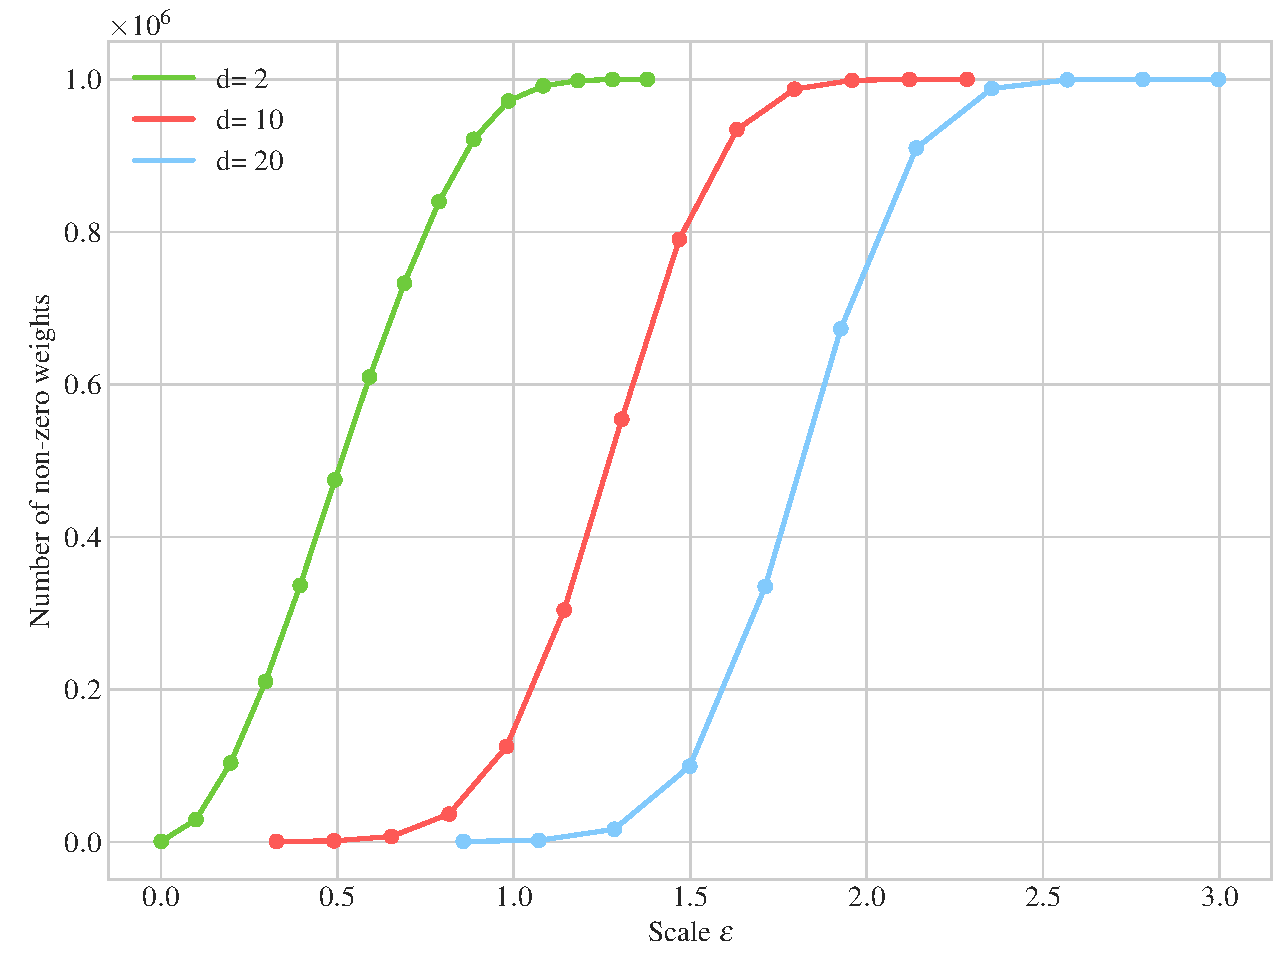
\includegraphics[width=.5\textwidth]{code/SSL/NNZ.pdf}
\caption{Dependence of the number of non-zero edges on the scaling parameter $\gscale$. Here, we sample $n\in\N$ points uniformly in the cube $[0,1]^d$ and only connect connect vertices $x_i,x_j\in\domain_n$ if $\norm{x_i-x_j}_2 < \gscale$. The plots shows the behavior for $d=2,10,20$.}\label{fig:graphscale}
\end{figure} 
%
%
Therefore, from a practical point of view $\gscale$ should be chosen relatively small. However, showing consistency of graph-based SSl algorithms often requires scaling assumptions that permit the desired length scales \cite{GarcSlep15, slepcev2019analysis, calder2019consistency}. In \cref{sec:GConv} we give concrete examples of such scaling assumptions. One of the main goals of \cite{roith2022continuum, bungert2021uniform} was to show convergence and rates at the smallest possible length scale, which was indeed achieved.
%
%
%
\begin{remark}{}{}
In many practical applications graph weights connecting all points within $\gscale$-ball of Euclidean distance are inferior to knn graphs \cite{calder2020poisson, flores2019algorithms, calder2022improved}. While most consistency results employ the $\gscale$-ball setting, recently, the authors in \cite{calder2022improved} were able to show convergence rates in the knn setting. In this thesis we focus on the $\gscale$-ball setting, however it is an interesting open question to transfer the results of \cite{roith2022continuum, bungert2021uniform, bungert2022ratio} to the knn setting.
\end{remark}
%
%
%
%
\subsection{The $p$-Laplacian: Continuum and Graph}\label{sec:pLap}
%
%
The archetype of learning methods we consider in the following is so-called \emph{Laplacian learning}, which had one of its first appearances in 
\cite{zhu2003semi}. The associated problem was given as
%
\begin{gather}\label{eq:SSL_Laplacian}
	\begin{gathered}
		\min_{\vec u:\domain_n\to\R} \sum_{x,y\in\domain_n} w_n(x,y)^2 
		\left(\vec u(y) - \vec u(x) \right)^2\\
		\text{subject to } \vec u(x) = \vec g(x) \text{ for all } x\in\conset_n.
	\end{gathered}
\end{gather}
%
%
%
Here, we always assume non-negative weights $w_n:\domain_n\times\domain_n\to[0,\infty)$. The intuitive idea behind this method is that it minimizes a discrete approximation of the Dirichlet energy and should therefore enforce a certain kind of \enquote{smoothness} of the solution $\vec u$. In \cite{zhou2005regularization} it was proposed to generalize the idea of the graph Dirichlet energy in \cref{eq:SSL_Laplacian} to arbitrary $1\leq p < \infty$ motivated by the continuum counterpart. While The contributions in \cite{roith2022continuum, bungert2021uniform, bungert2022ratio} mainly consider the case of $p=\infty$, the case $p<\infty$ serves as a  motivation for the whole discussion. Therefore, we briefly review the situation in the following. Here, we first introduce the continuum setting and then discuss the situation on the graph.
%
%
%
%
\paragraph{Continuum Setting}
We follow the exposition in \cite{lindqvist2017notes}. Let $\domain\subset\R^d$ be a bounded domain, then we consider the $p$-Dirichlet energy for functions $u\in W^{1,p}(\domain)$,
%
\begin{align}\label{eq:DirichletEnergy}
	\pDir{}_{p,\rho}(u) := \int_\domain \abs{\nabla u}^p \rho(x)^2 \, dx,
\end{align}
%
%
where $\rho:\domain\to\R$ is some given function. In the setting of \cite{GarcSlep15, slepcev2019analysis} $\rho$ denotes the density of data distribution as in \cref{sec:GSSL}. For $\rho\equiv1$ we simply write $\pDir{}_{p,1}=\pDir{}_{p}$. The associated variational problem is given in the following.
%
\begin{problem}{Variational Formulation}{prob:VarForm}
	For $p\in (1,\infty)$ and $V\subset W^{1,p}(\domain)$ find $u\in W^{1,p}(\domain)$ such that
	%
	\begin{align*}
		\pDir{}_{p,\rho}(u) \leq \pDir{}_{p,\rho}(v)
	\end{align*}
	%
	for all $v$, such that $(u-v)\in W^{1,p}_0$.
\end{problem}
%
\noindent%
Assume for simplicity that $\rho\equiv 1$ and that $u\in V$ is a minimizer of the above problem, then its first variation must vanish, i.e., for all $\phi\in C^\infty_0(\domain)$ one has
%
\begin{align}\label{eq:weakLap}
	\int_\domain \langle \abs{\nabla u}^p \nabla u, \nabla \phi \rangle \, dx = 0.
\end{align}
%
A function $u\in V$ satisfying \cref{eq:weakLap} is called a \emph{weak solution} of the $p$-Laplace equation. In fact, if $u$ 
is smooth enough one has that
%
\begin{align}\label{eq:strongLap}
	\Delta_p u := \div(\abs{\nabla u}^{p-2} \nabla u) = 0
\end{align}
%
where $\Delta_p$ is called the $p$-Laplacian. Boundary conditions on $\partial \domain$ given by a function $g\in W^{1,p}(\domain)$  can be incorporated by considering the set
$V_g := \{u\in W^{1,p}(\domain): u-g \in W^{1,p}_0(\domain)\}$. 
We state the following classical result, which can for example be found in \cite{lindqvist2017notes}.
%
\begin{theorem}{Existence and Uniqueness}{}
	For $p\in (1,\infty)$ and $g\in W^{1,p}(\domain)$ there exists a unique minimizer $u\in V_g$ of the $p$-Dirichlet energy, i.e.,
	%
	\begin{align*}
		\argmin_{u\in V_g} \pDir{}_p(u) = u.
	\end{align*}
	%
	Moreover, $u$ is a weak solution of the $p$-Laplace equation and there exists a function $\tilde{u}\in C(\domain)$ such that
	$u = \tilde{u}$ a.e. in $\domain$. If $g\in C(\domain)$ and $\domain$ is sufficiently smooth, then 
	$\tilde{u}\vert_{\partial \domain} = g\vert_{\partial \domain}$.
\end{theorem}
%
%
\begin{proof}
	The proof can be found in \cite[Thm. 2.16]{lindqvist2017notes}.
\end{proof}
%
%
\paragraph*{Local Minimization Property} Let $u$ solve \cref{prob:VarForm} for given boundary values $g\in W^{1,p}(\domain)$ and let $V\subset\subset\domain$ be a sufficiently regular subset. Then we have that
%
\begin{align*}
\pDir_p(u) = \int_{V} \abs{\nabla u}^p dx + \int_{\domain\setminus V} \abs{\nabla u}^p dx.
\end{align*}
%
Now consider \cref{prob:VarForm} on $V$ with boundary values given by $u$ and denote by $v$ the solution of the problem. Since $u=v$ on $\partial V$ we can extend $v$ onto $\domain$ by setting $v=u$ in $\domain\setminus V$, which gives $v\in W^{1,p}(\domain)$. Therefore, we obtain
%
\begin{align*}
\pDir_p(v) = \int_{V} \abs{\nabla v}^p dx + \int_{\domain\setminus V} \abs{\nabla u}^p dx \leq 
\int_{V} \abs{\nabla u}^p dx + \int_{\domain\setminus V} \abs{\nabla u}^p dx = \pDir_p(u).
\end{align*}
%
Since $u$ was unique this yields $u|_V = v|_V$, and therefore we know that any solution on $\domain$ solves \cref{prob:VarForm} also on any \enquote{nice} subset, with the boundary values given by itself. In \cref{sec:LipExt} we see that this \textit{local minimization property} does not hold automatically and has to enforced additionally. The underlying reason here is, that integrals are set-additive, but suprema are not, which is similarly explained in \cite{aronsson2004tour}.

%
%
\paragraph{Laplacian Learning} A natural extension of the problem given in \cref{eq:DirichletEnergy} is obtained by considering the target functional
%
\begin{align*}
	\GE^{w_n}_p(\vec u):= \sum_{x,y\in\domain_n} w_n(x,y)^p \abs{\vec u(y) - \vec u(x)}^p,
\end{align*}
%
which we refer to as the graph $p$-Dirichlet energy. Indeed, we notice structural 
similarities to the $p$-Dirichlet energy $\pDir_p$ in \cref{eq:DirichletEnergy}, replacing the integral by a finite 
sum and derivatives by weighted finite differences
%
\begin{align*}
	w_n(x,y)^p \abs{\vec u(y) - \vec u(x)}^p.
\end{align*}
%
This naturally leads to the following minimization problem.
%
\begin{problem}{Graph Energy Minimization}{prob:vargraph}
Given a weighted graph $(\domain_n, w_n)$ and a labeling function $\vec g:\conset_n\to\R$, for $\conset_n\subset\domain_n$ we consider 
the problem
%
\begin{align*}
	\min_{\vec u:\domain_n\to\R} \GE^{w_n}_p(\vec u) \text{ subject to } \vec u(x) = \vec g(x) \text{ for all } x\in\conset_n.
\end{align*}
\end{problem}
%
\noindent%
Since every function $\vec u:\domain_n\to\R$ can be identified with a vector $\vec u\in\R^n$, the above problem 
is in fact an optimization problem in $\R^n$. The functional $\GE^{w_n}_p:\R^n\to\R$ is bounded from below by $0$, continuous, convex and in the case $p>1$ even differentiable. However, one can prove unique existence with techniques very similar to the continuum case in \cite{lindqvist2017notes}. We give the adapted prove below for completeness. The important property to establish uniqueness is that the graph is connected to the boundary, i.e., for every $x\in\domain_n$ there exists a path $x=\gamma_1,\ldots,\gamma_m=o\in\domain_n$ with $w(\gamma_{i+1}, \gamma_i)>0$ connecting $x$ to a point $o\in\conset_n$ in the boundary. This is very intuitive, since on any connected component that does not communicate with the boundary, an arbitrary constant minimizes the \enquote{graph gradient}.
%
%
\begin{theorem}{Existence and Uniqueness}{} Let $(\domain_n,w_n)$ be a graph with non-negative weights, that is connected to its boundary $\conset_n\subset\domain_n$. Then \cref{prob:vargraph} admits a unique solution $\vec u:\domain_n\to\R$.
\end{theorem}
%
\begin{proof}
The	proof is an adaption from the continuum case in \cite[Thm. 2.16]{lindqvist2017notes}. We start by proving uniqueness, 	
Let $E = \{(x,y): w_n(x,y)>0\}$ be the set of all active edges and denote by $\nabla^{w_n} \vec u \in \R^{\abs{E}}$
%
\begin{align*}
(\nabla^{w_n} \vec u)_{(x,y)} := w_n(x,y) \left(\vec u(y) - \vec u(x)\right)
\end{align*}
%
the \enquote{graph gradient} on $E$, where we have that
%
\begin{align*}
\GE^{w_n}_p (\vec u) = \sum_{(x,y)\in E} w_n(x,y)^p \abs{\vec u(y) - \vec u(x)}^p 
= \sum_{(x,y)\in E} \abs{(\nabla^{w_n} \vec u)_{(x,y)}}^p=
\norm{\nabla^{w_n}\vec u}_p^p.	
\end{align*}
%
%
Let $\vec u_1, \vec u_2$ be two  solutions of \cref{prob:vargraph}, i.e. $\GE^{w_n}_p (\vec u_1)= \GE^{w_n}_p (\vec u_2)$. Since $\vec u_1,\vec u_2$ fulfill the boundary conditions, this also holds for $1/2(\vec u_1 + \vec u_2)$ and therefore $\GE^{w_n}_p(\vec u_1)\leq\GE^{w_n}_p(1/2(\vec u_1 + \vec u_2))$.


Assume that there exists $(\bar x,\bar y)\in E$ such that $\nabla^{w_n} \vec u_1(\bar x,\bar y)\neq \nabla^{w_n}\vec u_2(\bar x,\bar y)$, then we have that
%
\begin{align*}
\GE^{w_n}_p (\vec u_1) &\leq \GE^{w_n}_p \left(\frac{\vec u_1 + \vec u_2}{2}\right) =
\norm{\frac{\nabla^{w_n} \vec u_1(x,y) + \nabla^{w_n} \vec u_2(x,y)}{2}}^p_p\\
&<
\frac{1}{2} \sum_{(x,y)\in E\setminus\{(\bar x,\bar y)\}} \abs{\nabla^{w_n} \vec u_1(x,y)}^p + \abs{\nabla^{w_n} \vec u_2(x,y)}^p
\\ 
&\qquad+\frac{1}{2} \abs{\nabla^{w_n} \vec u_1(\bar x, \bar y)}^p + \abs{\nabla^{w_n} \vec u_2(\bar x, \bar y)}^p\\
&= 
\frac{1}{2}\left(\GE^{w_n}_p (\vec u_1) + \GE^{w_n}_p (\vec u_2)\right) 
= \GE^{w_n}_p (\vec u_1),
\end{align*}
%
which is a contradiction. Here, we employed the strict convexity of $t\mapsto \abs{t}^p$ which implies $\abs{t+\bar t}^p \leq 2^{p-1} \left(\abs{t}^p + \abs{\bar t}^{p}\right)$, where the inequality is sharp if $t\neq \bar t$. Therefore, we obtain that $\nabla^{w_n} \vec u_1 = \nabla^{w_n}\vec u_2$, which yields
%
\begin{align}\label{eq:diffid}
\vec u_1(y) - \vec u_1(x) = \vec u_2(y) - \vec u_2(x) \qquad\text{for all}\qquad (x,y)\in E.
\end{align}
%
Since $(\domain_n, w_n)$ is connected to $\conset_n$ for any $x\in\domain_n$ we can find a path $x=\gamma_1,\ldots,\gamma_m=o$ connecting $x$ to a point $o\in\conset_n$. By definition $w_n(\gamma_{i+1}, \gamma_i) >0$ for all $i=1,\ldots, m-1$ and therefore using \cref{eq:diffid} we obtain
%
\begin{align*}
\vec u_1(\gamma_{i}) - \vec u_1(\gamma_{i+1}) = \vec u_2(\gamma_{i}) - \vec u_2(\gamma_{i+1}) \qquad\text{for all}\qquad i=1,\ldots,m-1.
\end{align*}
%
which together with the boundary conditions $\vec u_1(o)=\vec u_2(o)=\vec g(o)$ yields
%
\begin{align*}
\vec u_1(x) = 
\vec u_1(\gamma_1)= \vec u_1(\gamma_1) &- \vec u_1(\gamma_2) + \vec u_1(\gamma_2)\\
%
=\ldots=\Bigg[\sum_{i=1}^{m-1} \vec u_1(\gamma_{i}) &- \vec u_1(\gamma_{i+1})\Bigg] + 
\vec u_1(o)\\
= \Bigg[\sum_{i=1}^{m-1} \vec u_2(\gamma_{i}) &- \vec u_2(\gamma_{i+1})\Bigg] + 
\vec u_2(o)\\
%
=\vec u_2(x)\phantom{---}&
\end{align*}
%
Since $x\in\domain_n$ was arbitrary, we get $\vec u_1 = \vec u_2$.\par
%
\noindent%
To show existence, we do not need to assume that the graph is connected to the boundary. On every connected component $V\subset \domain_n$ that is not connected to $\conset$ we can set $\vec u(x) = c$ for all $x\in V$, where $c\in\R$ is an arbitrary constant. We can select all edges in $V$, i.e. $E_V := E \cap V^{\times 2}$ ans since $V$ was a connected component---i.e. it does not have active edges to vertices outside of $V$---we can also split up the functional
%
\begin{align*}
\GE^{w_n}_{p}(\vec u) = \sum_{(x,y)\in E\setminus E_V} \abs{\nabla^{w_n} \vec u(x,y)}^p
+
\underbrace{\sum_{(x,y)\in E_V} \abs{\nabla^{w_n} \vec u(x,y)}^p}_{=0} = 
\sum_{(x,y)\in E\setminus E_V} \abs{\nabla^{w_n} \vec u(x,y)}^p
\end{align*}
%
where the contribution on the connected component is zero, since we set $\vec u$ to be constant here. Therefore, w.l.o.g. we can assume that $\domain_n$ is connected to the boundary, since any component not connected to boundary does not contribute to the problem. Let now $\vec u:\domain_n\to\R$ be a function and for $x\in\domain_n$ let $\gamma \in \domain_n^{\times m}$ be a path to a point in the boundary $o^x\in\conset_n$, then we have that
%
\begin{gather*}
\abs{\vec u(x)}^p \leq C\left(\sum_{i=1}^{m^x-1}\abs{\vec u(\gamma_{i}) - \vec u(\gamma_{i+1})}^p + \abs{\vec g(o^x)}^p\right) \leq 
C\left(\GE^{w_n}_p(\vec u) + \abs{\vec g(o^x)}^p\right)
\end{gather*}
%
where $C>0$ is a generic constant---not depending on $\vec u$---that also accounts for the factor $\left(\min_{(x,y)\in E}w_n(x,y)\right)^{-1}$. Summing over all $x\in\domain_n$ yields

\begin{gather*}
\norm{\vec u}^p_p = \sum_{x\in\domain_n} \abs{\vec u(x)}^p \leq 
C\left( n\, \GE^{w_n}_p(\vec u) + \sum_{x\in\domain_n} \abs{\vec g(o^x)}^p\right)\\
%
\leq  C \bigg(\GE^{w_n}_p(\vec u) + \norm{\vec g}^p_p\bigg).
\end{gather*}
%
Let now $\vec u_j$ denote a sequence such that
%
\begin{align*}
\GE^{w_n}_p(\vec u_j) \leq I + 1/j,\qquad\text{ where }\qquad
I := \inf_{\vec u=\vec g\text{ on } \conset_n} \GE^{w_n}_p(\vec u).
\end{align*}
%
Then we have that
%
\begin{align*}
\norm{\vec u_j}^p_p \leq C\ (\GE^{w_n}_p(\vec u_j) + \norm{\vec g}^p_p)
\leq C\ (I + 1/j + \norm{\vec g}^p_p) \leq \tilde C
\end{align*}
%
$j\in\N$, i.e. $\vec u_j$ is a uniformly bounded sequence of vectors in the finite dimensional space $\R^n$, and therefore there exists a subsequence---which we do not relabel---that converges to some $\vec u^\ast\in\R^n$. Since the functional $\GE^{w_n}_p:\R^n\to\R$ is continuous we obtain that
%
\begin{align*}
\GE^{w_n}_p(\vec u^\ast) = \lim_{j\to\infty} \GE^{w_n}_p(\vec u_j) = I
\end{align*}
%
which yields existence.
\end{proof}
%
%
\paragraph{The Graph Laplacian}
%
In the continuum case one considers the Euler--Lagrange equation for the functional $\pDir_p$, which yields the 
$p$-Laplacian, see \cref{sec:pLap}. Analogously, the optimality conditions for the graph $p$-Dirichlet energy $\GE^{w_n}_p:\R^n\to\R$ for $p > 1$ yield
%
\begin{align*}
\nabla_{\vec u} \GE^{w_n}_p(\vec u) = 0
\end{align*}
%
where for $x\in\domain_n$ we have 
\begin{align*}
\left(\nabla_{\vec u} \GE^{w_n}_p(\vec u)\right)_x =:\Delta^{w_n}_p \vec u(x)= \sum_{y\in\domain_n} w_n(x,y)^p \abs{\vec u(y) - \vec u(x)}^{p-2} \left( \vec u(y) - \vec u(x) \right)
\end{align*}
%
which is referred to as the graph $p$-Laplacian operator. This yields the following problem.
%
\begin{problem}{Graph $p$-Laplacian}{prob:graphLaplace}
	Given a weighted graph $(\domain_n, w_n)$ and a labeling function $\vec g:\conset_n\to\R$ with $\conset_n\subset\domain_n$, find 
	a function $\vec u:\domain_n\to\R$ such that
	%
	\begin{align*}
		\Delta_p^{w_n} \vec u &= 0, \text{ in } \domain_n\setminus \conset_n,\\
		\vec u &= \vec g \text{ on } \conset_n.
	\end{align*}
\end{problem}
%
\noindent%
Since the functional $\GE^{w_n}_p$ has a unique minimizer subject to the constraints given by $\vec g$ and the graph $p$-Laplacian is derived 
via optimality conditions, one expects that the \cref{prob:vargraph} and \cref{prob:graphLaplace} are equivalent. This is formulated in the following 
theorem.
%
\begin{theorem}{Existence and Uniqueness}{}
Let $(\domain_n,w_n)$ be a graph with non-negative weights, that is connected to its boundary $\conset_n\subset\domain_n$. Then there exists a unique solution $\vec u:\domain_n\to\R$ to \cref{prob:graphLaplace}, which also is the unique minimizer of \cref{prob:vargraph}.
\end{theorem}
%
\begin{proof}
This statement can be proven similarly to \cite[Theorem 5.3]{elmoataz2015p}.
\end{proof}
%
%
%
%
%
\subsection{Consistency for Graph-based SSL}\label{sec:CSSL}
%
%
While the graph 2-Laplacian has been successfully employed for classification tasks, see e.g. \cite{zhu2003semi, zhou2005regularization}, it has been observed that solutions tend to degenerate for large amounts of data, whenever $d\geq 2$ \cite{nadler2009statistical, alamgir2011phase, el2016asymptotic}. We illustrate this phenomenon in \cref{ex:pLapBad}.
%
\begin{figure}
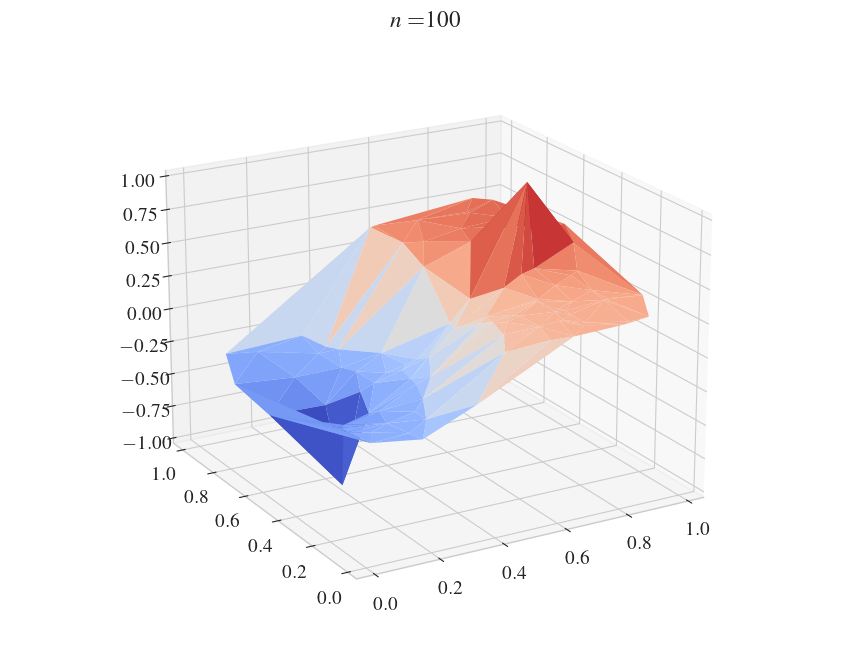
\includegraphics[width=.28\textwidth, trim={3.1cm 1cm 3.5cm 0cm},clip]{code/SSL/2Dex_100.png}%
\hfill%
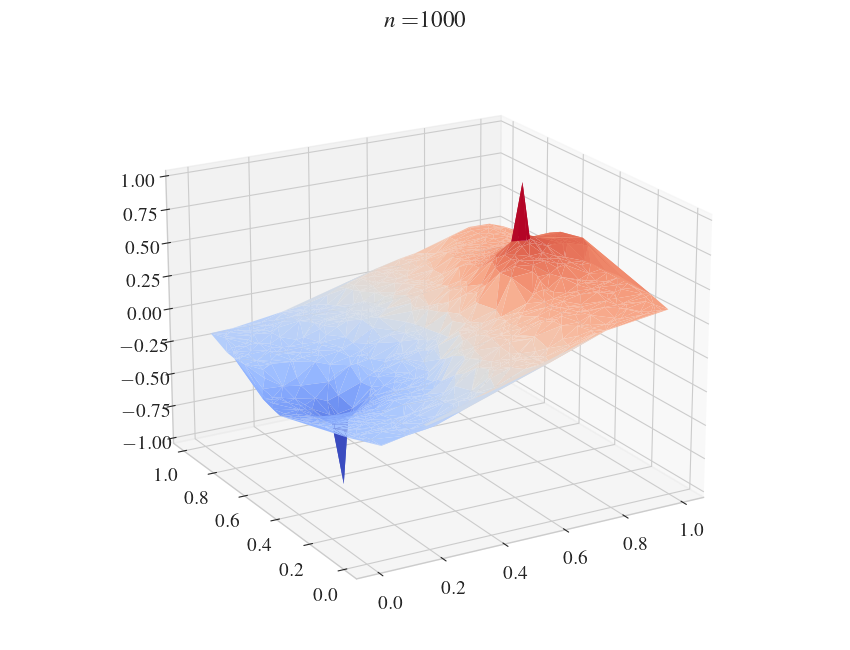
\includegraphics[width=.28\textwidth,trim={3.1cm 1cm 3.5cm 0cm},clip]{code/SSL/2Dex_1000.png}%
\hfill%
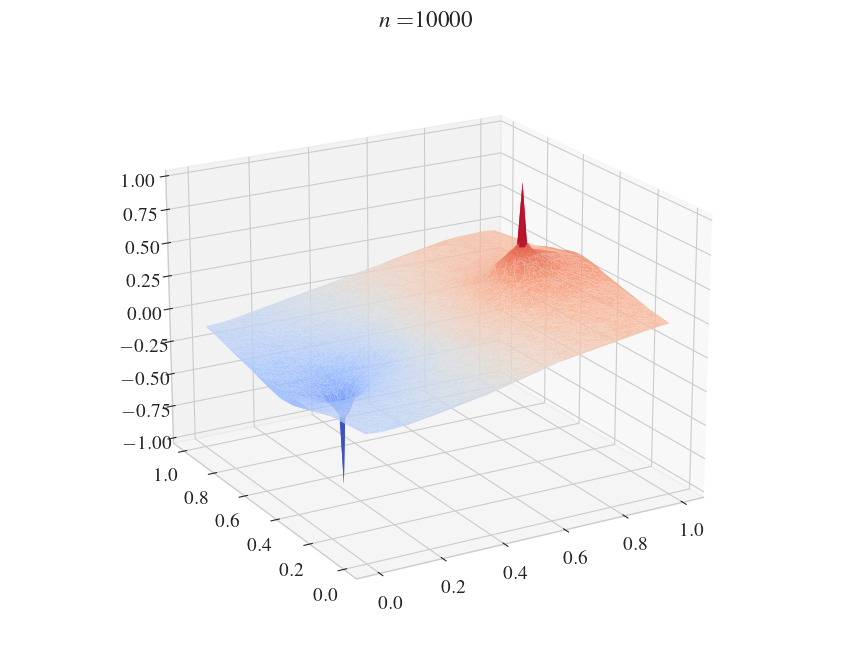
\includegraphics[width=.28\textwidth,trim={3.1cm 1cm 3.5cm 0cm},clip]{code/SSL/2Dex_10000.png}%
%
\caption{Solution to the Laplacian Learning problem ($p=2$) for different number of data points $n\in\{100,1000,10000\}$.}\label{fig:pdeg}
\end{figure}
%
%
\begin{example}{}{ex:pLapBad}
We sample different number of points $n\in\{100,1000,10000\}$ in $(0,1)^2$ and keep a fixed constraint on $\conset_n=\{o_1, o_2\}=\{(0.2,0.5), (0.8, 0.5)\}$ with $\vec g(o_1) = -1, \vec g(o_2)=1$. In \cref{fig:pdeg} we observe that for increasing $n$ the solution $\vec u$ of \cref{eq:SSL_Laplacian} tends to be a constant equal to the average of the given constraints and spike at the given constraints.
\end{example}
%
%
\noindent%
This observation motivates the driving question of this chapter and the works presented:
%
\begin{center}
\textit{%
Are Semi-Supervised Learning algorithms consistent in the infinite data limit?}
\end{center}
%
In our case \enquote{consistency} roughly ask the discrete solutions to converge to the continuum counterparts they are motivated by, in the data limit $n\to\infty$. Here, we distinguish between point-wise consistency as in \cite{von2008consistency, gine2006empirical, hein2005graphs}, consistency on a function space level \cite{slepcev2019analysis, GarcSlep15,calder2019consistency, roith2022continuum, bungert2021uniform} and consistency of a discretized operator \cite{calder2019consistency, bungert2022ratio}. We detail the notion of consistency in the following.  
%
%
\paragraph{Consistency for the $p$-Laplacian} 
As observed in \cite{nadler2009statistical, alamgir2011phase, el2016asymptotic} the question of consistency is now connected to the relation between $p$ and $d$, where one considers the three regimes $p<d$, $p=d$ and probably the most relevant case $p>d$. The $p$-Dirichlet problem in the continuum can be formulated as a variational problem in $W^{1,p}$. However, it is important to remember that in our setting we most likely consider pointwise constraints on a discrete set $\conset$ even in the continuum. In order to impose pointwise constraints, one requires that functions in $W^{1,p}$ exhibit some continuity properties. By the Sobolev embedding theorem, this is the case when $p>d$, \cite{adams2003sobolev}. This leads to a first qualitative intuition that consistency can only be achieved in the case $p>d$. We note that $p$-harmonic functions are actually more regular also in the case $p\leq d$, beyond the implication of the Sobolev embedding theorem. However, this regularity does not help for the continuum limits \cite{nadler2009statistical, alamgir2011phase, el2016asymptotic}.

The most relevant result for our contribution in \cite{roith2022continuum} is the $\Gamma$-convergence statement of \cite{GarcSlep15}, which considers a clustering task, via the TV functional. Here, the authors show 
%
\begin{align*}
\frac{1}{\gscale_n n^2}\, \GE^{w_n}_1 \xrightarrow{\phantom{-}\Gamma\phantom{-}} \sigma_\eta\, \pDir_{1,\rho}
\end{align*}
%
where the constant $\sigma_\eta$ is defined as in \cref{eq:kernelconst}. We review details on $\Gamma$-convergence in \cref{sec:GConv}. The important insight here, is that the graph scaling $\gscale_n$ must not tend to zero too fast. We quickly provide some intuition to this fact:
%
\begin{itemize}
	\item Problems on the graph are non-local, communication between points takes place on a finite scale.
	\item In the limit we want to obtain a local problem, communication takes place at a infinitesimal small scale.
	\item If the graph scale $\gscale_n$ tends to zero too fast, there is not enough communication between vertices, or even worse the graph becomes disconnected.
\end{itemize}
%
The optimal scaling obtained in \cite{GarcSlep15} for $d\geq 3$ is given as 
%
\begin{align}\label{eq:garcscaling}
\lim_{n\to\infty} \left(\frac{\log n}{n}\right)^{1/d}\, \gscale_n^{-1} = 0,
\end{align}
%
i.e. $\gscale_n$ must go to zero slower than $\left(\frac{(\log n)}{n}\right)^{1/d}$. This scaling is optimal, in the sense that the graph is disconnected with high probability if $\gscale_n < \lambda \left(\frac{\log n}{n}\right)^{1/d}$, see \cite{GarcSlep15}. The main difference here, is however that the considered clustering task does not directly involve a given labeling on the set $\conset_n\subset\domain_n$. This setting was considered in \cite{slepcev2019analysis}, where first the generalization of the $\Gamma$-convergence statement in \cref{eq:garcscaling} was provided. Furthermore, the authors then consider the constrained  model by incorporating the boundary conditions into the functional
%
\begin{align*}
\GE^{w_n, \text{cons}}_p(\vec u) :=
\begin{cases}
\GE^{w_n}_p(\vec u) &\text{if } \vec u = \vec g \text{ on }\conset_n,\\
\infty &\text{else}.
\end{cases} 
\end{align*}
%
%
In order to show $\Gamma$-convergence of the constrained functionals, an additional upper bound on the scaling has to be assumed. This means that the graph scaling must not tend to zero too slowly, namely
%
\begin{align*}
n\, \gscale_n^p \xrightarrow{n\to\infty} 0.	
\end{align*}
%
Together, with \cref{eq:garcscaling} this then implies
%
\begin{align*}
n^{-1/d} \ll \gscale_n \ll n^{-1/p}
\end{align*}
%
which is only possible if $p>d$. Therefore, one again obtains well-posedness of the constrained problem, if $p$ is large enough.


\paragraph{Sending $p$ to Infinity} 

Since the assumption that $p>d$ is crucial for asymptotic consistency, a natural idea is to send $p$ to $\infty$ and analyze the corresponding limit problem. This yields the so-called \emph{Lipschitz learning} task \cite{von2004distance, kyng2015algorithms}, which is the main point of interest in this chapter. We formalize this problem in \cref{sec:LipExt}. In \cref{fig:pinf} we observe that for $p=\infty$ we indeed obtain smoother solutions, compared to \cref{fig:pdeg}. In this regard Lipschitz learning seems promising to overcome the consistency issue.

\begin{figure}
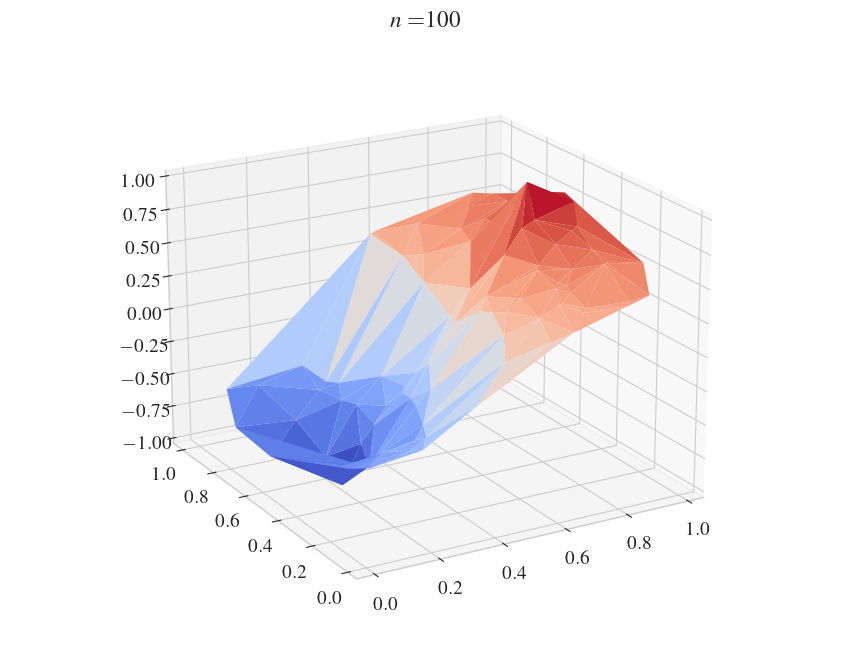
\includegraphics[width=.28\textwidth, trim={3.1cm 1cm 3.5cm 0cm},clip]{code/SSL/2Dex_100-p=inf.png}%
\hfill%
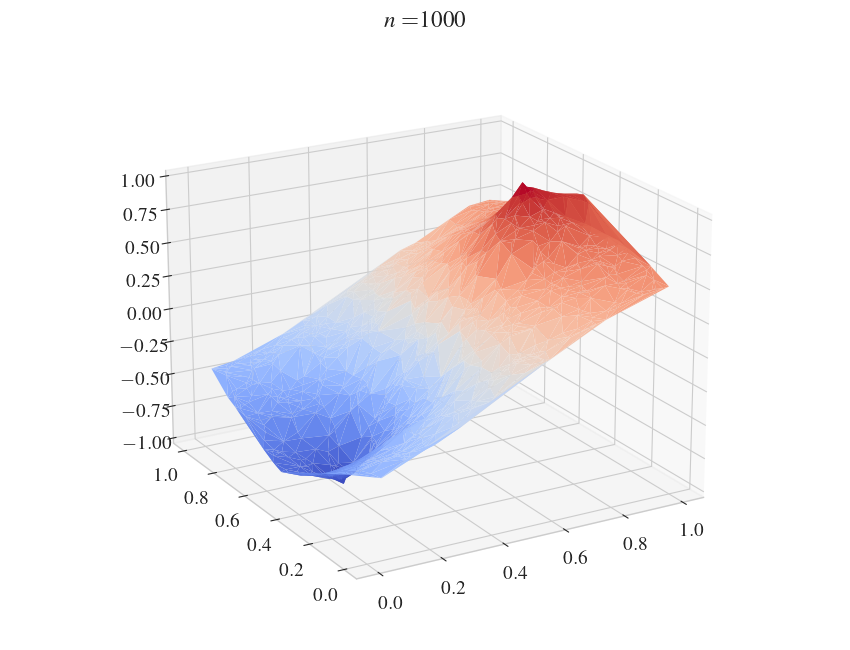
\includegraphics[width=.28\textwidth,trim={3.1cm 1cm 3.5cm 0cm},clip]{code/SSL/2Dex_1000-p=inf.png}%
\hfill%
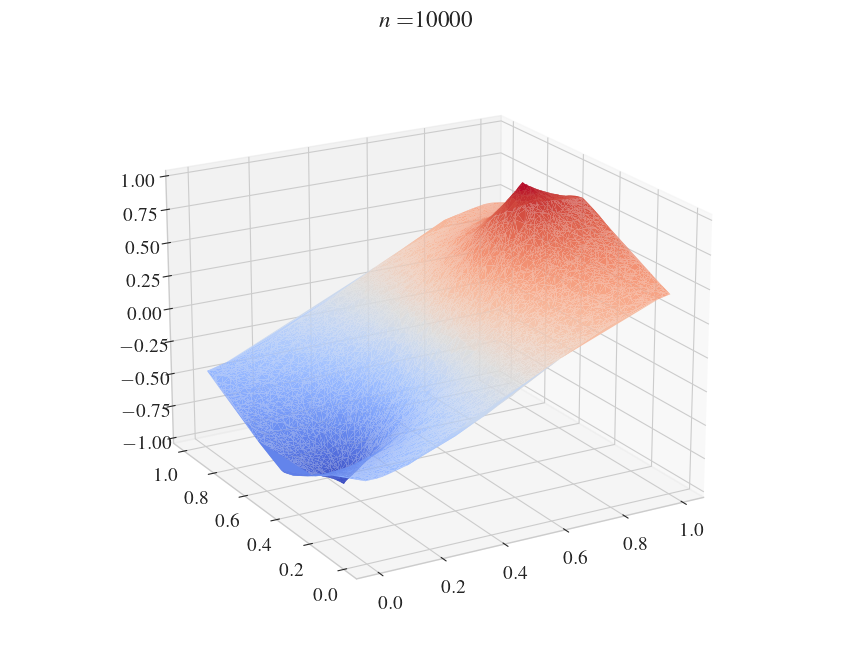
\includegraphics[width=.28\textwidth,trim={3.1cm 1cm 3.5cm 0cm},clip]{code/SSL/2Dex_10000-p=inf.png}%
%
\caption{Solution to the Laplacian Learning problem ($p=\infty$) for different number of data points $n\in\{100,1000,10000\}$. The setup is otherwise copied from \cref{ex:pLapBad}.}\label{fig:pinf}
\end{figure}
%
However, as already noticed in \cite{el2016asymptotic} being a pure $L^\infty$ problem, Lipschitz learning does not respect the density of data in any way. Namely, the method is exclusively distance based. This behavior is a drawback in many machine learning applications. However, by carefully rescaling the graph weights one obtains a data sensitive problem, see \cite{calder2019consistency} and \cref{sec:GConv}. 

The contributions presented in this chapter are all connected to the Lipschitz learning task. Namely, we are able to show consistency and convergence rates under very mild scaling assumptions.
%
%
%
%
%
%
%
\section{Lipschitz Extensions and the Infinity Laplacian: Continuum and Graph}\label{sec:LipExt}
%
Our main point of interest in this chapter is the Lipschitz learning task and its continuum limit. In this section we first motivate the continuum problem as considered in \cite{roith2022continuum, bungert2021uniform, bungert2022ratio}. We then given some details on the discrete problem.
%
%
\subsection{The Continuum Setting}\label{sec:LipExtCont}
%
%
We first recall, that for 
$u\in W^{1,\infty}(\domain)$ we have that
%
\begin{align*}
\lim_{p\to\infty} \pDir{}_{p,\rho}(u)^{1/p} = \esssup_{x\in\supp(\rho)} \abs{\nabla u(x)} =: \pDir{}_{\infty,\rho}(u),
\end{align*}
%
see \cite{jensen1993uniqueness}. Again, we see that that the weighting $\rho$ only enters via its support, therefore we do not explicitly consider it in the following and instead assume $\domain=\supp(\rho)$ and then only write $\pDir{}_{\infty}$. The functional $\pDir{}_\infty$ is weak$^*$-lower semi-continuous over $W^{1,\infty}(\domain)$, (see e.g. \cite[Thm. 2.6]{barron2001lower}). In the classical theory developed by Jensen in \cite{jensen1993uniqueness} one considers the following problem, which is tries to \enquote{minimize the \emph{sup-norm} of the gradient} as described by Jensen.
%
\begin{problem}{Gradient Sup-Norm Problem}{prob:gradsup}
For an open domain $\domain\subset\R^d$ find a function $u\in W^{1,\infty}(\domain)$ such that
%
\begin{align*}
\norm{\nabla u}_\infty \leq \norm{\nabla v}_\infty \text{ for every } v, \text{s.t. } (u-v)\in W^{1,\infty}_0.
\end{align*}
\end{problem}
%
\noindent%
This problem can be seen as the limit problem for $p\to\infty$ of \cref{prob:VarForm}. Additionally imposing boundary conditions with $g:\partial\domain\to\R$, \cite{jensen1993uniqueness} then draws the connection to so-called \emph{Lipschitz extensions}, which are the driving concept in this section. We introduce a more general viewpoint---that does not require the notion of a gradient---later on, but first introduce the variational problem. 

\paragraph{The intrinsic metric and the Lipschitz constant.}

As noticed in \cite{jensen1993uniqueness} working with the Lipschitz constant and the sup-norm of the gradient requires a careful 
treatment of the distance measurement. Let $\tilde\domain$ be a set and let $d(\cdot,\cdot)$ be a semi-metric on $\tilde\Omega$, that is $d(\cdot,\cdot)$ fulfills 
the requirement of a metric up to triangle inequality. Then we define the Lipschitz constant of a function $u:V\to \R$ on a subset $V\subset \tilde\domain$ as
%
\begin{align*}
\Lip_d(u; V):= \sup_{x,y\in V, x\neq y} \frac{\abs{u(x) - u(y)}}{d(x,y)}.
\end{align*}
%
If $d(\cdot,\cdot)$ denotes the Euclidean distance we omit the subscript. i.e. $\Lip_d = \Lip$. Additionally, we can 
introduce the space of Lipschitz functions $\Lip_d(V)$ on $V$ via 
$u\in \Lip_d(V) \Leftrightarrow \Lip_d(u;V) <\infty$.
%
\begin{remark}{Lipschitz and Sobolev functions}{}
If $\domain\subset\R^d$ is sufficiently regular, e.g., it has Lipschitz boundary then we have that
%
\begin{align*}
\Lip(\domain) = W^{1,\infty}(\domain),
\end{align*}
%
where this identity is of course to be understood in the sense of equivalence classes in $\L^p$ spaces. We refer to \cite{evans2018measure} for a proof of this result.
\end{remark}
%
The above remark already relates Lipschitz with $W^{1,\infty}$ functions. Often however, we need a quantitative 
comparison between the Lipschitz constant and the sup-norm of the gradient of a function. Here, it is essential 
which distance measure is chosen for the Lipschitz constant. For an open domain $\domain\subset\R^d$ we have the inequality
%
\begin{align*}
\norm{\nabla u}_\infty \leq \sup_{x\neq y} \frac{\abs{u(x) - u(y)}}{\abs{x-y}}
\end{align*}
%
which can be proven via the definition of the gradient. For the reverse inquality, one has to respect the 
geometry of the domain, namely for $x,y\in\domain$ we have that
%
\begin{align}\label{eq:LipGrad}
\abs{u(x) - u(y)} \leq \norm{\nabla u}_\infty\ d_\domain(x,y)
\end{align}
%
see, e.g., \cite[Prop9.3, Rem. 7]{brezis2011functional}, where
%
\begin{align*}
d_\domain(x,y) = \inf \left\{
\int_0^1 \abs{\dot{\gamma}(t)} dt : \gamma\in C^1([0,1], \domain)\text{ with } \gamma(0)=x, \gamma(1) =y
\right\}
\end{align*}
%
denotes the \emph{geodesic distance} on $\domain$. If $\domain$ is convex, we have that $d_\domain(x,y) = \abs{x-y}$ for every 
$x,y\in \domain$ and therefore \cref{eq:LipGrad} yields $\Lip(u) = \norm{\nabla u}_\infty$. However, this situation changes for non-convex domains, see \cref{ex:tube}. Additionally it is often necessary to define 
a distance measure on the closure of $\domain\subset\R^d$. In order to have a geodesic on $\overline{\domain}$ one can simply consider $d_{\overline{\domain}}$, see e.g. \cite{bungert2021uniform}, which then yields the length space $(\overline{\domain}, d_{\overline{\domain}})$. In the classical theory developed in \cite{jensen1993uniqueness} one alternatively considers
%
\begin{align*}
\tilde{d}_{\overline{\domain}}(x,y) := \liminf_{(\tilde x,\tilde y)\to(x,y)} d_\domain(\tilde{x},\tilde{y}).
\end{align*}
%
The differences between these notions are demonstrated in the following example. Also note, that $\tilde{d}_{\overline{\domain}}$ is only a semi-metric on $\overline{\domain}$ since it is lacking a triangle inequality.
%
\begin{example}{}{ex:tube}
For $I = [-\pi, c]\cup [c, \pi]$ with $c=\pi/6$ we consider the domain
%
\begin{align*}
\bigcup_{\theta \in I} B_1\left((\cos(\theta),\sin(\theta)\right)
\end{align*}
%
which is visualized in \cref{fig:tube} and the points $x=(2\, c, 1), y= (2\, c, -1)$. The 
line segment between $x$ and $y$ contains the point $z=(2\, c, 0)$, however $z\notin \domain$. One can show that 
the geodesic has the length $d_\domain(x,y) = 4\, \cos(\pi/6) + \pi \approx 6.606$ which is the length of the dotted path 
in \cref{fig:tube}. However, we observe that 
%
\begin{align*}
\overline{\domain} = \bigcup_{\theta \in I } 
\overline{B_1\left((\cos(\theta),\sin(\theta)\right)}
\end{align*}
%
and in particular $z\in \overline{B_1\left((c,c)\right)}$, therefore $d_{\overline{\domain}}(x,y) = 2$.
\end{example}
%
\begin{figure}
\centering
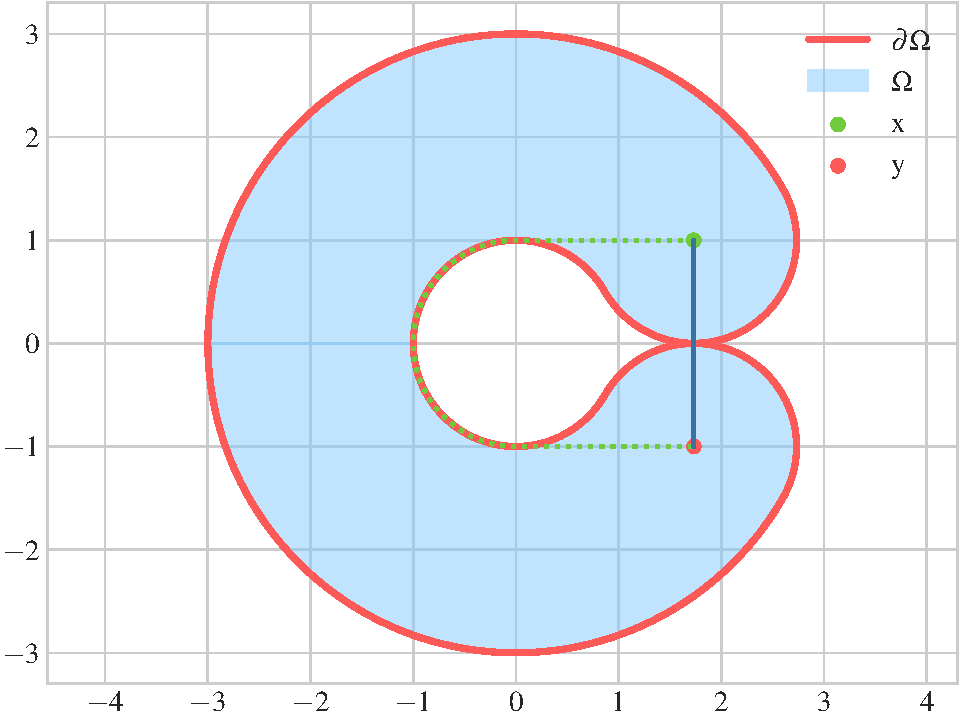
\includegraphics[width=.5\textwidth]{code/domains/tube.pdf}
\caption{The domain in \cref{ex:tube}.}\label{fig:tube}
\end{figure}
%
%
\paragraph{Solutions to the Gradient Sup-Norm Problem} Before generalizing the theory of Lipschitz extension to arbitrary metric spaces, we first note, that one can explicitly construct solutions of \cref{prob:gradsup}. Namely, for given $g\in\Lip(\partial\domain)$ the functions 
%
\begin{align}\label{eq:JenSol}
\begin{aligned}
\overline{g}(x) &:= \inf_{y\in\partial\domain} g(y) + 
\Lip_{\tilde{d}_{\overline{\domain}}}(g; \partial\domain)\cdot \tilde{d}_{\overline{\domain}}(x,y)\\
%
\underline{g}(x) &:= \sup_{y\in\partial\domain} g(y) - 
\Lip_{\tilde{d}_{\overline{\domain}}}(g; \partial\domain)\cdot \tilde{d}_{\overline{\domain}}(x,y)
\end{aligned}
\end{align}
%
are solutions to the gradient sup-norm problem that coincide with $g$ on $\partial\domain$, see \cite[Th. 1.8]{jensen1993uniqueness}.
%
\begin{remark}{}{}
The same concept of constructing solutions is applied in the following sections in a more abstract setting. 
These solutions are then called Whitney and McShane or respectively maximal and minimal extensions, see 
\cref{lem:ext}.
\end{remark}
%
One easily observes that there are cases where $\overline{g}\neq \underline{g}$ and therefore the problem does not admit a unique solution. A concrete example, to showcase this phenomena is given in \cite[p. 53]{jensen1993uniqueness}.
%
%
\paragraph{Lipschitz Extensions in Metric Spaces} The problem considered in the last section was motivated by a variational problem for $\pDir_\infty(u)=\norm{\nabla u}_\infty$. However, the theory of Lipschitz extensions provides a more general framework. Namely, here we do not assume that $\domain$ is a subset of 
$\R^d$ and rather consider a metric space $(\tilde{\domain},d)$ with $\domain\subset \tilde\domain$. 
%
\begin{remark}{}{}
For applications within this thesis we have that $\domain\subset\R^d$ is an open bounded domain and then consider 
$\tilde\domain:= \closure\domain$, i.e., the closure of $\domain$ within the topology induced by the Euclidean distance. 
In this abstract setting however, we use any metric space $\tilde\domain$ while still being close notation wise.
\end{remark}
%
%
%
\noindent%
A result originally due to Kierszbraun \cite{Kirszbraun1934} states that for two Hilbert spaces $\Inp, \Oup$, a subset $\conset\subset \Inp$ and a function $g:\conset\to \Oup$ there exists a function $u:\Inp\to \Oup$ such that 
%
\begin{align*}
u &= g \text{ on } \mathcal{O},\\
\Lip(u; \Inp) &= \Lip(g; \conset).
\end{align*}
%
Here, the metrics for the respective Lipschitz constants are induced by the inner products of the Hilbert spaces. We refer to \cite{Kirszbraun1934} for the original proof and to \cite[Th. 1.31]{Schwartz1969} for a proof of the version as stated above.
In this work we only consider the case $\Oup=\R$ which allows for more general assumption on the space $\Inp$. We now formulate the Lipschitz extension problem in our setting.
%
\begin{problem}{Lipschitz Extensions}{prob:Lipext}
Let $(\tilde{\domain},d)$ be a metric space and $\conset\subset \tilde{\domain}$ be a bounded subset. For a given Lipschitz function $g:\conset\to\R$ find a Lipschitz function $u:\tilde\domain\to \R$ such that
%
\begin{align*}
\Lip_d(u; \tilde\domain) = \Lip_d(g; \conset).
\end{align*}
%
A function $u:\tilde{\domain}\to\R$ with this property is called \emph{Lipschitz extension} of 
$g$ to $\tilde{\domain}$.
\end{problem}
%
\noindent%
In this setting one can explicitly construct solutions of the Lipschitz extension task. They are not unique, however one has an upper and a lower bound. In fact, conceptually these solutions 
are very similar to the functions in \cref{eq:JenSol} and even coincide, whenever the sup-norm of the gradient is given as the Lipschitz constant.
%
\begin{lemma}{}{lem:ext}
In the setting of \cref{prob:Lipext} we have that the 
%
\begin{itemize}
\item \textbf{Whitney (or maximal) extension:} $\Whit{g}(x) := \inf_{y\in \conset} g(y) + \Lip_d(g; \conset)\cdot d(x,y)$ and the
\item \textbf{McShane (or minimal) extension:} $\McS{g}(x) := \sup_{y\in \conset} g(y) - \Lip_d(g; \conset)\cdot d(x,y)$
\end{itemize}
%
defined for $x\in\tilde\domain$ are Lipschitz extensions of $g$ to $\tilde\domain$. Moreover, let $u:\tilde\domain\to\R$ be any Lipschitz extension of 
$g$, the we have that
%
\begin{align*}
\McS{g} \leq u \leq \Whit{g}.
\end{align*} 
\end{lemma}
%
\begin{proof}
We refer to \cite{whitney1992analytic} and \cite{mcshane1934extension} for the proofs of the respective result.
\end{proof}
%
\noindent%
As demonstrated in \cref{ex:maxprinc}, there are cases where $\Whit{g}\neq\McS{g}$ and 
therefore, Lipschitz extensions are not unique in general. Furthermore, \cite{aronsson2004tour} points out that the Whitney and McShane extension do not allow for a comparison principle, which can also be observed in \cref{ex:maxprinc}.
%
\begin{example}{}{ex:maxprinc}
Consider the set $\tilde\domain = [-1,1]$ and $\conset=\{-1,0,1\}$ with 
%
\begin{align*}
\color{apple}g_1\bc(x)&:= 0,\\
\color{grape}g_2\bc(x)&:= 1/2\ (x- \abs{x}),\\
\color{sky}g_3\bc(x)&:= -\color{grape}g_2\bc.
\end{align*}
%
Then we have that $\color{grape}g_2\bc\leq \color{apple}g_1\bc$ on $\conset$ but 
%
\begin{align*}
\color{grape}\Whit{g_2}\bc>\color{apple} \Whit{g_1}\bc \text{ in } (0,1),
\end{align*}
%
see \cref{fig:maxprinc} for a visualization. Analogously, we have that $\color{sky}g_3\bc\geq \color{apple}g_1\bc$ on $\conset$ but 
%
\begin{align*}
\color{sky}\McS{g_3}\bc<\color{apple} \McS{g_1}\bc \text{ in } (0,1).
\end{align*}
\end{example}
%
\begin{figure}
\centering
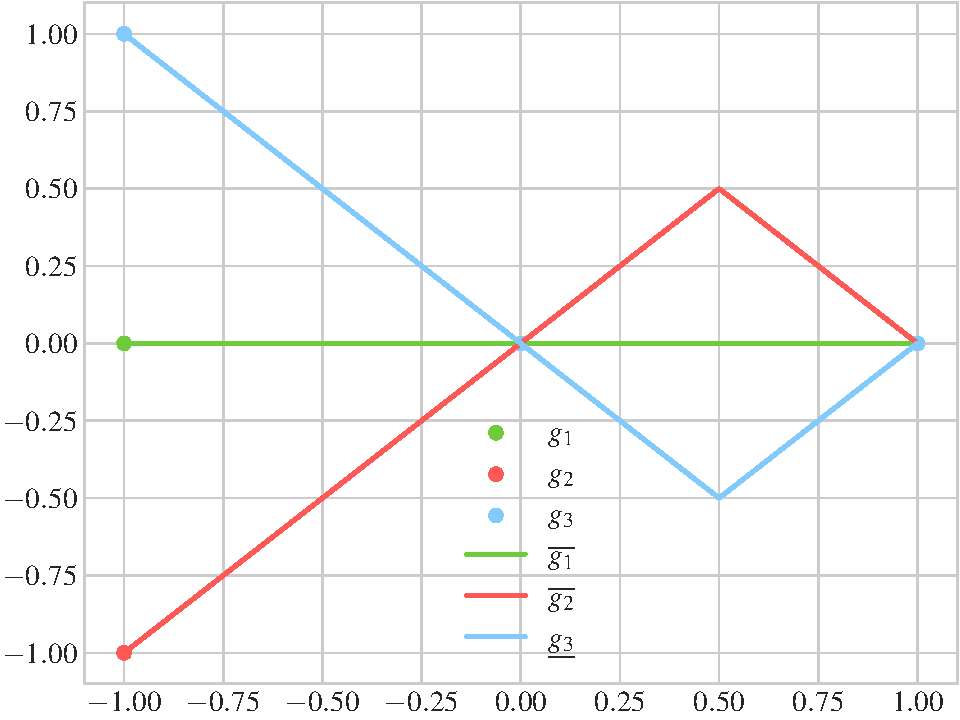
\includegraphics[width=.5\textwidth]{code/lipextcomp/comp.pdf}
\caption{The maximal extension does not admit a comparison principle, as demonstrated in \cref{ex:maxprinc}.}\label{fig:maxprinc}
\end{figure}
%
%
\paragraph{Absolutely Minimizing Extension}\label{sec:AMLE}
%
Sending $p\to\infty$ in the variational formulation of the $p$-Laplace equation 
yields the Lipschitz extension task, which however does not admit for unique solutions. So the question arises, which property is lost in the limit case. For $p<\infty$ one has the local minimization property, as explained in \cref{sec:CSSL}. This lead Aronsson to introduce the concept of \emph{absolutely minimizing Lipschitz extension} in \cite{aronsson1967extension}, by additionally enforcing the minimizing property on every subset. A function $u\in W^{1,\infty}$ is called absolutely minimal, iff
%
\begin{align}\label{eq:absmin}
\esssup_{x\in V} \abs{\nabla u} \leq \esssup_{x\in V} \abs{\nabla v} \text{ for every open } V\subset \domain
\end{align}
%
and every function $v$ such that $(u-v)\in W^{1,\infty}_0$. In fact in \cite{aronsson1967extension} it is also shown, that 
$u_p\xrightarrow{p\to\infty} u_\infty$ (), which seems to validate the notion of absolute minimizers. In \cite{aronsson2004tour} it was shown, that one has an equivalent formulation involving the Lipschitz constant. For a given Lipschitz function $g:\overline{\domain}\to\R$ we have that $u_\infty$ with $(u_\infty-g)\in W^{1,\infty}_0(\domain)$ fulfills \cref{eq:absmin} iff
%
\begin{align*}
\Lip(u_\infty; V) \leq \Lip(v; V) \text{ for every } V\subset \domain
\end{align*}
%
and every function $v$ such that $(u-v)\in W^{1,\infty}_0(V)$, see \cite{aronsson1967extension}. In this thesis we work with a notion of absolute minimizers, which is equivalent to the above formulation for convex domains in $\R^d$. However, for our applications it is more convenient to formulate the problem for abstract length spaces.
%
\begin{problem}{AMLEs}{prob:amles}
Let $(\tilde{\domain}, d)$ be a length space, $\conset\subset\tilde{\domain}$ a closed subset and $g:\conset\to\R$ a Lipschitz function. Find an extension $u\in C(\tilde{\domain})$ such that $u=g$ on $\conset$ and
%
\begin{align*}
\Lip_d(u; \overline{V}) = \Lip_d(u, \partial V) \text{ for all open and connected sets } V\subset \tilde{\domain}\setminus \conset.
\end{align*}
%
A function $u$ fulfilling this property is called absolutely minimizing Lipschitz extension of $g$.
\end{problem}
%
\begin{remark}{}{}
In our setting $\domain$ is an open subset of $\R^d$ and we then choose $\tilde{\domain} = \overline{\domain}$. Here, it is important to note that 
the topological notions like boundary and interior are to be understood relative to $\overline{\domain}$. A visualization of this concept can be found in \cref{fig:relb}.
\end{remark}
%
\begin{figure}
\begin{center}
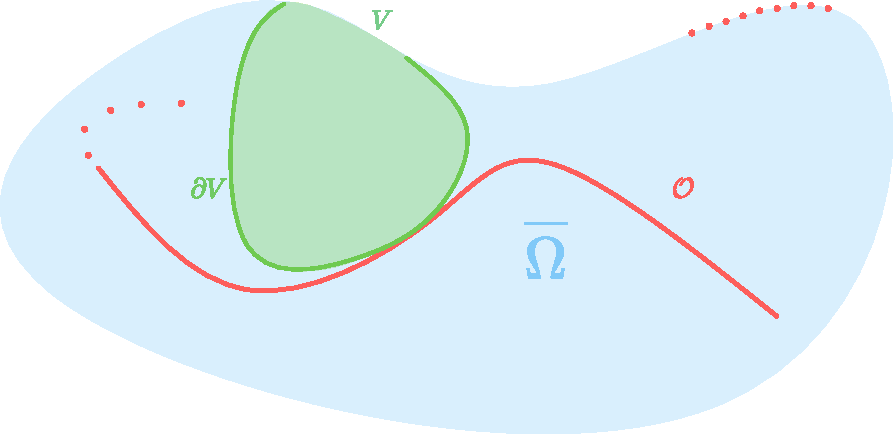
\includegraphics[width=.7\textwidth]{atelier/SSL/relboundary.pdf}
\end{center}
\caption{A set $V\subset\overline{\domain}$ can be relatively open w.r.t. the metric space $\overline{\domain}$ although, $V\cap\partial\domain \neq\emptyset$, where $\partial \domain$ is the boundary within the standard topology on $\R^d$. The relative boundary of $\partial_{\overline{\domain}} V$ does not include any parts of $\partial \domain$.}\label{fig:relb}
\end{figure}
%
%
\paragraph{The Infinity Laplacian} In the Euclidean case one can derive an operator equation by considering the limit of the $p$-Laplacian operator. This yields the $\infty$-Laplacian which is defined as
%
\begin{align*}
\Delta_\infty u = \langle \nabla u, D^2 u\, \nabla u\rangle = 
\sum_{i,j} \partial_{x_i} u\, \partial_{x_j} u\, \partial_{x_i,x_j} u
\end{align*}
%
for functions of class $C^2$. Intuitively this operator gives the second derivative of $u$ into the direction of its gradient. This then yields the infinity Laplace equation.
%
\begin{problem}{}{}
Let $\domain\subset\R^d$ 
\end{problem}
Solutions are typically considered in the viscosity sense, see e.g. \cite{aronsson2004tour}, where one can also show that solving the infinity Laplace equation
%
\begin{align*}	
\end{align*}

 
%For any vector $v\in\R^n$ and $h\in\R^+$ we can employ the Taylor approximation to see that
%%
%\begin{align*}
%u(x + h\, v) + u(x - h\, v) - 2u(x) = \langle v, D^2 u\, v\rangle + o(h^2)
%\end{align*}


%
%

\paragraph{Comparison with Cones} As shown in \cite{aronsson2004tour} the concept of absolutely minimizing extensions is equivalent to so-called \emph{comparison with cones}. For some metric $d(\cdot,\cdot)$ a cone function is defined as
%
\begin{align*}
x\mapsto a\, d(x,z) + c
\end{align*}
%
where $z$ denotes the origin or cone tip, $a$ its opening angle and $c$ some offset. The property we consider in the following basically asks, if a function $u$ is smaller than a cone on the boundary of some set $V$ not including the tip $z$, then it should be smaller also in the interior of the domain. This means for any $a,c\in\R$ and $z\notin V$ we have the implication
%
\begin{align*}
u \leq a\, d(x,z) + c \text{ on }\partial V \Rightarrow
u \leq a\, d(x,z) + c \text{ in } V
\end{align*}



%
%

\subsection{Graph Lipschitz Extensions}\label{sec:GLipExt}
%
We now consider the limit $p\to\infty$ of \cref{prob:vargraph} in the graph case. Analogously to \cref{sec:InfLip} we derive
%
\begin{align*}
\lim_{p\to\infty} \left(\GE^{w_n}_p(\vec u)\right)^{1/p}= \max_{x,y\in\domain_n} w_n(x,y) \abs{\vec u(y) - \vec u(x)}=:\GE^{w_n}_\infty(\vec u)
\end{align*}
%
which extends the graph $p$-Laplacian energy to the case $p=\infty$. Again we notice structural similarities to 
the continuum version $\pDir_\infty$. 
%
\begin{remark}{}{}
Informally speaking the functional $\GE$ combines elements of a gradient and Lipschitz constant. Assuming that $w_n(x,y)$ relates to $\abs{x-y}$ we see that the finite difference approximation
resembles a Lipschitz constant. However, typically $w_n(x,y)$ has also some localizing property which fits the interpretation of a gradient better.
\end{remark}
%
This functional now leads to the graph Lipschitz extension problem.
%
\begin{problem}{Graph Energy Minimization}{prob:lipgraph}
Given a weighted graph $(\domain_n, w_n)$ and a labeling function $\vec g:\conset_n\to\R$, for $\conset_n\subset\domain_n$ we consider 
the problem
%
\begin{align*}
\min_{\vec u:\domain_n\to\R} \GE_\infty^{w_n}(\vec u) \text{ subject to } \vec u(x) = \vec g(x) \text{ for all } x\in\conset_n.
\end{align*}
\end{problem}
%
\noindent%
Since the weighting function $w_n:\domain_n\times\domain_n\to\R^+_0$ does not induce a metric, \cref{prob:lipgraph} does not directly fit the framework of the abstract Lipschitz Extension in \cref{prob:Lipext}. However, we can consider paths in $(\domain_n, w_n)$, connecting arbitrary $x,y\in\domain_n$ i.e. vectors $\gamma\in\domain_n^{\times k}$ such that 
%
\begin{align*}
w_n(\gamma_i, \gamma_{i+1}) &> 0\quad\text{for all } i=1,\ldots, k-1,\\
\gamma_1 &= x, \\ \gamma_k &= y
\end{align*}
%
for which we define the length as
%
\begin{align*}
\abs{\gamma} = \sum_{i=1}^{k-1} w(\gamma_i, \gamma_{i+1})^{-1}.
\end{align*}
%
This yields the metric space $(\domain_n, d_{w_n})$, where $d_{w_n}:\domain_n\times\domain_n\to\R$ is defined as
%
\begin{align}\label{eq:graphdist}
d_{w_n}(x,y) := \min \left\{ \abs{\gamma}: \gamma \text{ is a path in } 
(\domain_n, w_n)\text{ from } x \text{ to } y\right\}.
\end{align}
%
\begin{remark}{}{}
We note that it is important to only consider non-negative weights, otherwise any loop with a negative \enquote{length} would decrease the 
length of the whole path arbitrarily. However, restricting ourselves to non-negative weights we can easily see, that the minimum in \cref{eq:graphdist} is indeed attained.
\end{remark}
%
With this definition we can consider the Lipschitz extension task of $g:\conset_n\to\R$ to $\domain_n$ within the metric space $(\domain_n,d_{w_n})$, i.e. within the setting of \cref{prob:Lipext}. Therefore the question arises, whether the minimization problem in \cref{prob:lipgraph} is equivalent to the metric Lipschitz extension problem for which we have the following lemma.
%
%
\begin{lemma}{}{}
For a graph $(\domain_n, w_n)$ with non-negative weights and a function $\vec u:\domain_n\to\R$ we have that 
\begin{align*}
\GE_\infty^{w_n}(\vec u) = \Lip_{d_{w_n}}(\vec u).
\end{align*}
%
Furthermore, for $\conset_n\subset\domain_n$ and a function $\vec g:\conset_n\to\R$ and we have that
%
\begin{align*}
\vec g = \vec u \text{ on } \conset_n\Rightarrow
\Lip_{d_{w_n}}(\vec g;\conset_n) \leq \Lip_{d_{w_n}}(\vec u).
\end{align*}
\end{lemma}
%
%
\begin{proof}
\textbf{Step 1:} We show that $\Lip_{d_{w_n}}(\vec u) \leq \GE_\infty^{w_n}(\vec u)$.\\
%
We can choose a path $\gamma\in\domain_n^{\times k}$ such that
%
\begin{align*}
\Lip_{d_{w_n}}(\vec u) &= \frac{\vec u(\gamma_1) - \vec u(\gamma_k)}{\abs{\gamma}}.
\end{align*}
%
The path $\gamma$ allows to compare vertices $\gamma_1, \gamma_k\in\domain_n$ that aren't necessarily neighbors in the graph. However, each consecutive vertices in the path are neighbors in the graph and therefore we have
%
\begin{align}\label{eq:gebound}
w_n(\gamma_i, \gamma_{i+1}) \abs{\vec u(\gamma_{i+1}) - \vec u(\gamma_i)}
&\leq \GE^{w_n}_\infty(\vec u)\quad \text{ for all } i=1,\ldots, k-1.
\end{align} 
%
We now employ an elementary result for numbers $a_i\in\R^+_0, b_i\in\R^+, i=1,\ldots m\in\N$, namely
%
\begin{align}\label{eq:basicineq}
\left[
a_i\cdot b_i \leq c\in\R \quad\text{ for }
i=1,\ldots, m
\right]
%
\Rightarrow 
%
\frac{\sum_{i=1}^{m}a_i}{\sum_{i=1}^{m} b_i^{-1}} \leq c
\end{align}
%
which can be seen as follows
%
\begin{align*}
a_i\cdot b_i &\leq c\quad\text{ for } i=1,\ldots, m\\
\Rightarrow
a_i &\leq b_i^{-1}\cdot c \quad\text{ for } i=1,\ldots, m\\
\Rightarrow\sum_{i=1}^{m} a_i &\leq \left(\sum_{i=1}^m b_i^{-1}\right)\cdot c\\
%
\Rightarrow\frac{\sum_{i=1}^{m} a_i}{\sum_{i=1}^{m} b_i^{-1}} &\leq c.
\end{align*}
%
This then yields 
%
\begin{align*}
\frac{\abs{\vec u(\gamma_1) - \vec u(\gamma_k)}}{\abs{\gamma}}\leq
\frac{\sum_{i=1}^{k-1} \abs{\vec u(\gamma_i) - \vec u(\gamma_{i+1})}}{\abs{\gamma}} = 
\frac{\sum_{i=1}^{k-1} \abs{\vec u(\gamma_i) - \vec u(\gamma_{i+1})}}{\sum_{i=1}^{k-1} w_n(\gamma_i, \gamma_{i+1)^{-1}}}
%
\leq
\GE^{w_n}_\infty(\vec u) 
\end{align*}
%
where in the last inequality we employed \cref{eq:basicineq} together with \cref{eq:gebound}.\\
%
\noindent%
\textbf{Step 2:} We show that $\Lip_{d_{w_n}}(\vec u) \geq\GE_\infty^{w_n}(\vec u)$.\\
%
Let $x,y\in \domain_n$, then we know that $d_w(x,y) \leq w_n(x,y)^{-1}$ and therefore
%
\begin{align*}
\abs{\vec u(x) - \vec u(y)} w_n(x,y)\leq 
\frac{\abs{\vec u(x) - \vec u(y)}}{d_w(x,y)} \leq 
\max_{\bar{x}, \bar{y}\in\domain_n}  
\frac{\abs{\vec u(\bar x) - \vec u(\bar y)}}{d_w(\bar x,\bar y)} = \Lip_{d_{w_n}}(\vec u).
\end{align*}
%
Since this holds for arbitrary $x,y\in\domain_n$ we have that
%
\begin{align*}
\GE^{w_n}_\infty(\vec u) = \max_{x,y\in\domain_n} \abs{\vec u(x) - \vec u(y)} w_n(x,y)
\leq
\Lip_{d_{w_n}}(\vec u).
\end{align*}\\
\noindent%
\textbf{Step 3:} We show that $\Lip_{d_{w_n}}(\vec g;\conset_n) \leq \Lip_{d_{w_n}}(\vec u)$.\\
%
If $\vec g = \vec u$ on $\conset$ this simply follows since the maximum for the Lipschitz constant of $\vec u$ is taken over a larger set. Indeed,

\begin{align*}
\Lip_{d_{w_n}}(\vec u) &= 
\max_{x,y\in\domain_n} \frac{\abs{\vec u(x) - \vec u(y)}}{d_w(x,y)}
\geq 
\max_{x,y\in\conset_n} \frac{\abs{\vec u(x) - \vec u(y)}}{d_w(x,y)}
=
\max_{x,y\in\conset_n} \frac{\abs{\vec g(x) - \vec g(y)}}{d_w(x,y)}\\
&=
\Lip_{d_{w_n}}(\vec u; \conset_n).
\end{align*}
\end{proof}
%
%
%
This lemma shows that the abstract Lipschitz extension task considered on the metric space $(\domain_n, d_{w_n})$ and the Graph $\infty$-Dirichlet minimization task are indeed equivalent. Therefore, we also have the Whitney and McShane extensions
%
\begin{align*}
\Whit{\vec g}(x) &= \inf_{y\in\conset_n} \vec g (y) + d_{w_n}(x,y)\\
\McS{\vec g}(x) &= \sup_{y\in\conset_n} \vec g (y) - d_{w_n}(x,y)
\end{align*}
%
as solutions on the graph. Analogously, the problem does not admit for unique solutions.
%
%
%
\paragraph{Absolutely Minimizing Graph Extensions}
%
Similarly to \cref{sec:AMLE} we can now consider absolutely minimizing extensions. However, the problem in 
\cref{prob:amles} uses a notion of a boundary and it is not directly clear how to infer this concept to the discrete set $\domain_n$. Therefore, we define the following what we mean by \enquote{boundary} on a graph.
%
\begin{definition}{}{}
Let $(\domain_n, w_n)$ be a weight graph and let $V\subset\domain_n$ be a subset, then we define
%
\begin{itemize}
\item the \textbf{exterior} boundary as $\partialext :=\{x\in \domain_n\setminus V: w_n(x,y) > 0 \text{ for some } y\in V\}$,
\item the \textbf{interior} boundary as $\partialint :=\{x\in V: w_n(x,y) > 0 \text{ for some } y\in \domain_n\setminus V\}$.
\end{itemize}
%
The closure of $V$ is then defined as $\extcl{V} V := V\cup \partialext$ and the interior as 
$\stackrel{\circ}{V}^{\text{int}}:= V\setminus \partialint V$.
\end{definition}
%
%
We note that it is not possible to define a topology on $\domain_n$ that would yield the above notions. Namely, the only admissible topology in our case would be the discrete topology, i.e., $2^{\domain_n}$. However, in this topology the only closed sets are $\emptyset$ and $\domain_n$ which is not useful for the applications in the following. Using the Kuratowski closure axioms \cite{kuratowski1922operation} we remark the following.
%
\begin{lemma}{}{}
The exterior closure on a weighted graph $(\domain_n, w_n)$ is a preclosure or Čech closure.
\end{lemma}
%
\begin{proof}
Here, we use the notion of a preclosure in \cite{vcech1966topological}.
We first see that $\overline{\emptyset}^{\text{ext}}=\emptyset$ and that $V\subset \overline{V}^{\text{ext}}$ for every subset $V\subset\domain_n$, i.e. the above defined closure preserves the empty set and is extensive. Furthermore, for two sets $V_1,V_2\subset \domain_n$ we have that
%
\begin{gather*} 
x\in \partialext (V_1\cup V_2)\\
\Leftrightarrow\left[x\notin V_1\cup V_2\right]\wedge \left[\exists y\in V_1\cup V_2: w_n(x,y) \right]\neq 0\\
\Leftrightarrow 
\left[x\notin V_1\cup V_2\right]\wedge
\bigg(\left[\exists y\in V_1: w_n(x,y) \neq 0 \right]\vee
\left[\exists y\in V_2: w_n(x,y) \neq 0 \right]\bigg)\\
\Leftrightarrow \left[x\in \partialext V_1\setminus V_2\right]\vee
\left[x\in  \partialext V_2 \setminus V_1 \right]\\
\Leftrightarrow x\in (\partialext V_1 \cup \partialext V_2)\setminus (V_1\cup V_2).
\end{gather*}
%
We have shown that $\partialext (V_1\cup V_2)=(\partialext V_1 \cup \partialext V_2)\setminus (V_1\cup V_2)$. Therefore, we have that
%
\begin{align*}
\extcl{V_1\cup V_2} &= 
V_1\cup V_2 \cup \partialext (V_1\cup V_2)\\
&= V_1\cup V_2 \cup ((\partialext V_1 \cup \partialext V_2)\setminus (V_1\cup V_2))\\
&= V_1\cup \partialext V_1 \cup V_2 \cup \partialext V_2\\
&= \extcl{V_1}\cup\extcl{V_2}.
\end{align*}
%
This shows that the closure preserves binary unions and therefore we have shown, that it is indeed a Čech closure.
\end{proof}
%
%
%
The missing property, that inhibits the closure to induce a topology is the so-called idempotence. Namely, there are sets $V\subset \domain_n$ such that
%
\begin{align*}
\overline{V}^{\text{ext}} \neq \extcl{\extcl{V}}.
\end{align*}
%
\begin{figure}
\centering
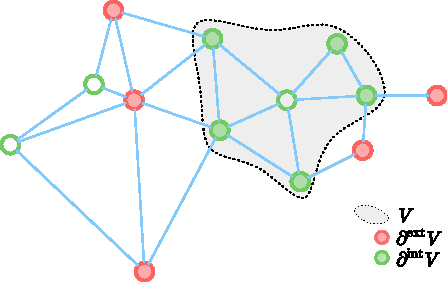
\includegraphics{atelier/SSL/boundary.pdf}
\caption{Visualization of exterior and interior boundary on a graph.}\label{fig:graphb}
\end{figure}
%
E.g. in the example visualized in \cref{fig:graphb} we see that $\overline{\overline{V}^{\text{ext}}}^{\text{ext}}=\domain_n\neq \overline{V}^{\text{ext}}$. Since the closure we employ here does not induce a topology, we have a slightly modified notion of absolutely minimizers.
%
\begin{problem}{Graph AMLEs}{prob:GAMLE}
Given a connected weighted graph $(\domain_n, w_n)$, $\conset_n\subset\domain_n)$ and a function $\vec g:\conset_n\to\R$ find a function $\vec u:\domain_n\to\R$ such that
%
\begin{align*}
\Lip_{d_{w_n}}(\vec u; \extcl{V}) &= \Lip_{d_{w_n}}(\vec u; \partialext V)
\text{ for all connected } V\subset \domain_n\setminus\conset_n,\\
\vec u &= \vec g\text{ on } \conset_n.
\end{align*}
\end{problem}
%
%
%
\paragraph{Comparison with graph Distance functions}
%
Analogously to the continuum case \cref{??} we can also consider comparison with distance functions on graphs. The main ingredients here, are the graph distance function $d_{w_n}$ and the notion of closure on a graph as developed in the last section.
%
%
\begin{definition}{}{}
For a weighted graph $(\domain_n,w_n)$ we say a function $\vec u:\domain_n\to\R$ fulfills comparison with distance function from above (CDFA) on a subset $U\subset \domain_n$ if for every $V\subset U$ we have
%
\begin{align}\label{eq:CDFA}\tag{CDFA}
\max_{\extcl{V}} \left(u + a\ d_{w_n}(\cdot, z)\right)=
\max_{\partialext V} \left(u + a\ d_{w_n}(\cdot, z)\right)
\end{align}
%
for every $z\in \domain_n\setminus V$ and every $a\in\R$. We say that $\vec u$ fulfills comparison with distance function from below (CDFB) on a subset $U\subset \domain_n$ if for every $V\subset U$ we have
%
\begin{align}\label{eq:CDFB}\tag{CDFB}
\min_{\extcl{V}} \left(u - a\ d_{w_n}(\cdot, z)\right)=
\min_{\partialext V} \left(u - a\ d_{w_n}(\cdot, z)\right)
\end{align}
%
for every $z\in \domain_n\setminus V$ and every $a\in\R$.
\end{definition}
%
%
Analogously to the continuum case, we say that a function fulfills comparison with distance functions, if it fulfills both, \cref{eq:CDFA} and \cref{eq:CDFB}. Existence of such functions is established later, we are first interested in the question of uniqueness. Since the notion of graph boundaries is not directly compatible with the usual definitions on metric spaces, we prove it separately. Here, we adapt arguments from [smart] and [LeGruyer]. To do so we first consider the operators
%
\def\eps{\varepsilon}
\begin{align*}
\vec S^\eps \vec u (x) := \max_{y\in\domain_n: d_{w_n}(x,y)\leq \eps} \vec u(y) \quad
\vec S_\eps \vec u (x) := \min_{y\in\domain_n: d_{w_n}(x,y)\leq \eps} \vec u(y)
\end{align*}
%
and proof the following lemma, which is the analogue of 

%
%
%
%
\paragraph{The Graph infinity Laplacian}
%
We can also obtain the limit of the Graph $p$-Laplace operator via the following formal calculation,
%
\begin{align*}
\Delta^{w_n}_p \vec u(x) &= 0\\
\Leftrightarrow \sum_{y\in\domain_n} w_n(x,y)^{p} \abs{\vec u(y) - \vec u(x)}^{p-2} (\vec u(y) - \vec u(x)) &= 0\\
%
\Leftrightarrow 
\sum_{y: \vec u(x)\leq \vec u(y)} w_n(x,y)^{p}(\vec u(y)-\vec u(x))^{p-1}
&= \sum_{y: \vec u(x)> \vec u(y)} w_n(x,y)^{p}(\vec u(x)-\vec u(y))^{p-1}.
%\\
%\Leftrightarrow
%\left(\sum_{y: \vec u(x)\leq \vec u(y)} w_n(x,y)^{p}(\vec u(y)-\vec u(x))^{p-1}\right)^{1/p}
%&=\\
%\left(\sum_{y: \vec u(x)> \vec u(y)} w_n(x,y)^{p}(\vec u(x)-\vec u(y))^{p-1}\right)^{1/p}
\end{align*}
%
Taking the terms on the left and right hand side to the power of $1/p$ and then formally sending $p\to\infty$ then yields
%
\begin{align*}
\max_{y: \vec u(x)\leq \vec u(y)} w_n(x,y)(\vec u(y)-\vec u(x)) &= 
\max_{y: \vec u(x) > \vec u(y)} w_n(x,y)(\vec u(x)-\vec u(y))\\
%
\Leftrightarrow \max_{y\in\domain_n} w_n(x,y)(\vec u(y)-\vec u(x)) &= 
-\min_{y\in\domain_n} w_n(x,y)(\vec u(y)-\vec u(x)).
\end{align*}
%
%
This calculation motivates the definition of the graph infinity Laplacian
%
\begin{align*}
\Delta_\infty^{w_n} \vec u(x) := \max_{y\in\domain_n} w_n(x,y)(\vec u(y)-\vec u(x)) +
\min_{y\in\domain_n} w_n(x,y)(\vec u(y)-\vec u(x)),
\end{align*}
%
which then allows to formulate the associated problem as an  extension of \cref{prob:graphLaplace}.

\begin{problem}{Graph $\infty$-Laplacian}{prob:graphinfLaplace}
Given a weighted graph $(\domain_n, w_n)$ and a labeling function $\vec g:\conset_n\to\R$ with $\conset_n\subset\domain_n$, find 
a function $\vec u:\domain_n\to\R$ such that
%
\begin{align*}
\Delta_\infty^{w_n} \vec u &= 0, \text{ in } \domain_n\setminus \conset_n,\\
\vec u &= \vec g \text{ on } \conset_n.
\end{align*}
\end{problem}
%
%
This problem is again well-posed, which is formulated in the following lemma.
%
\begin{lemma}{}{}
There exists a unique solution for \cref{prob:graphinfLaplace}.
\end{lemma}
%
%
\paragraph{Relation between the Graph Lipschitz Extensions}
We now establish the connection between the different notions of Lipschitz extensions. Compared to the continuum case we do not establish the full equivalences but only the necessary implications required for the convergence proofs in \cite{bungert2021uniform}.

First we see, that graph AMLEs are indeed special solutions of the basic Lipschitz extension problem on the graph.
%
\begin{lemma}{}{}
A graph AMLE is also a Lipschitz extension.
\end{lemma}
%
\begin{proof}

\end{proof}
%
%
We now state the main result concerning the relation between the graph infinity Laplacian, graph AMLEs and comparison cones.
%
%
\begin{lemma}{}{}
Let $(\domain_n,w_n)$ be a weighted connected graph and $\vec g:\conset_n\to\R$ be a given function for $\conset_n\subset\domain_n$. Furthermore, let $\vec u:\domain_n\to\R$ be graph infinity harmonic on $\domain_n\setminus\conset_n$ with boundary conditions given by $\vec g$, i.e., $\vec u$ solves \cref{prob:graphinfLaplace} then we have that
%
\begin{itemize}
\item $\vec u$ is an graph AMLE, i.e., $\vec u$ solves \cref{prob:GAMLE},
\item $\vec u$ fulfills comparison with cones.
\end{itemize}
\end{lemma}
%
%
\begin{proof}
Both of the stament are proven in \cite{bungert2021uniform}. From \cite[Prop. 3.8]{bungert2021uniform} we have that $\vec u$ is an graph AMLE. Furthermore, form \cite[Th. 3.2]{bungert2021uniform} we have that $\vec u$ fulfills comparison with cones. In fact, \cite[Th. 3.2]{bungert2021uniform}, shows a more refined statement, namely that
%
\begin{align*}
-\Delta^{w_n}_\infty \vec u &\leq 0 \Rightarrow \vec u \text{ fulfills CDFA},\\
-\Delta^{w_n}_\infty \vec u &\geq 0 \Rightarrow \vec u \text{ fulfills CDFB}.
\end{align*}
%
\end{proof}
%
%
%
%
%
%
%
%
%
\section{Gamma Convergence: \cite{roith2022continuum}}\label{sec:GConv}
We are now in the situation to present the main results of \cite{roith2022continuum, bungert2022ratio}. 
%
%
%
%
\paragraph{The kernel}

\begin{enumerate}[label=(K\upshape\arabic*)]
\item\label{en:K1} $\eta$ is positive and continuous at $0$,
\item\label{en:K2} $\eta$ is non-increasing,
\item\label{en:K4} $\supp(\eta) \subset [0,\etaradius_\eta]$ for some $\etaradius_\eta>0$.
\end{enumerate}
%
%
%
%
%
Originally, the concept of $\Gamma$-convergence dates back to De Giorgi \cite{de1975tipo} as a type of variational convergence. We refer to \cite{Brad02, dal2012introduction} for a detailed overview on this notion and related topics. While $\Gamma$-convergence was successfully employed in a pure continuum setting for a longer time (see e.g. \cite{modica1977esempio}), it was more recently used to prove convergence form a discrete to a continuum functional \cite{chambolle2010continuous, braides2012quantitative, van2012gamma}. The most relevant reference for this thesis was disruptive work presented by Garc\'ia Trillos and Slep\v{c}ev in \cite{GarcSlep15}. Here, the considered object was a graph total variation or generalized parameter, where the functional corresponds to $\GE^{w_n}_p$ for $p=1$ from \cref{prob:vargraph}. Among other important ideas and notions, we want to highlight two ingredients that directly influenced \cite{roith2022continuum}:
%
\begin{enumerate}[label=\arabic*)]
\item $\Gamma$-convergence on a common metric space, that allows to compare graph functions with continuum functions.
\item The proof strategy, discrete to non-local, non-local to continuum.
\end{enumerate}
%
%
We review how theses concepts influence \cite{roith2022continuum} in the following sections. The results in \cite{GarcSlep15} were later transferred to the case $1<p<\infty$ in \cite{slepcev2019analysis} and in this sense \cite{roith2022continuum} constitutes the generalization to $p=\infty$. \todo{G Convergence in L infty}
%
%
\paragraph{$\Gamma$-convergence}
%
We start with the basic definition of $\Gamma$-convergence.
%
%
\begin{definition}{$\Gamma$-convergence}{}
Let $X$ be a metric space and let $F_n:X\rightarrow [-\infty,\infty]$ be a sequence of 
functionals. We say that $F_n$ $\Gamma$-converges to the functional 
$F:X\rightarrow [-\infty,\infty]$ if
\begin{enumerate}[label=(\roman*)]
\item \textbf{(liminf inequality)} for every sequence $(x)_{n\in\N}\subset X$ converging to 
$x\in X$ we have that
\begin{align*}
\liminf_{n\rightarrow\infty} F_n(x_n) \geq F(x);
\end{align*}
\item\textbf{(limsup inequality)} for every $x\in X$ there exists a sequence 
$(x)_{n\in\N}\subset X$ converging to $x$ and 
\begin{align*}
\limsup_{n\rightarrow\infty} F_n(x_n)\leq F(x).
\end{align*}
\end{enumerate}
\end{definition}
%
%
In order to show convergence of discrete functions defined on $\domain_n$ to continuum functions acting on $\overline\domain$, one needs to define a common metric space. \cite{GarcSlep15} introduced the space $TL^p$
%
\begin{align*}
TL^p :=\left\{(\mu, u): \mu\in \mathcal{P}(\domain), u\in L^p(\mu)\right\}
\end{align*}
%
together with the transport distance
%
\begin{align*}
d_{TL^p}((\mu, u), (\nu, v)) = \inf_{\pi\in \Gamma(\mu,\nu)}
\left(\int_{\domain\times\domain} \abs{x-y}^p + \abs{u(x) - v(y)}^p d\pi(x,y)\right)^{1/p}
\end{align*}
%
where $\Gamma(\mu,\nu)$ is the set of coupling between $\mu$ and $\nu$. A sequence $(mu_n, u_n)$ converges to $(\mu,u)$ in $TL^p$ iff there exists a sequence of transportation maps $T_n:\domain\to\domain$ with $T_n\#\mu = \mu_n$ and 
%
\begin{align*}
\int_{\domain} \abs{x- T_n(x)} d\mu(x)\rightarrow 0
\end{align*}
%
such that $u_n\circ T_n \xrightarrow{L^p} u$, \cite[Prop. 3.12]{GarcSlep15}. Therefore, the maps $T_n$ allow to employ standard convergence in $L^p$. In order to transfer this situation to $L^\infty$ one could try to employ a $\infty$-Wasserstein distance. However, as argued in \cite{roith2022msc} the arguments do not transfer directly, since convergence in $W^\infty$ does not metrize weak convergence of measures \cite[Thm. 5.10]{santambrogio2015optimal}. However, as seen in \cite{roith2022continuum} one can employ a more direct argument. For problems in $L^p$ the conservation of mass was important for the maps $T_n$ (i.e. $T_n\#\mu = \mu_n$) such that the integrals could be transformed. This condition is irrelevant in $L^\infty$, namely we have the following analogous transformation rule in $L^\infty$.
%
\begin{lemma}{\cite[Lem. 2]{roith2022continuum}}{lem:suptrafo}
For two probability measures $\mu,\nu \in \mathcal{P}(\overline{\domain})$, a measurable map 
$T:\domain\rightarrow\domain$ which fulfills
\begin{enumerate}[label=\upshape(\roman*)]
\item $\nu<<T\#\mu$,
\item $T\# \mu<<\nu$,
\end{enumerate}
and for a measurable function $u:\domain\rightarrow\R$ we have that
\begin{align*}
\nu\operatorname{-}\esssup_{x\in\domain} u(x) = \mu\operatorname{-}\esssup_{y\in\domain} u(T(y)).
\end{align*}
\end{lemma}
%
%
We want to compare the discrete measure $\mu_n = \frac{1}{n}\sum_{x\in\domain_n} \delta_x$ to the target measure $\mu$. In this setting a closest point projection $p_n:\domain\to\domain_n$
%
\begin{align*}
p_n(x) \in \argmin_{y\in\domain_n} \abs{x- y}
\end{align*}
%
fulfills the assumption of \cref{lem:suptrafo}. This allows us to extend the functional $\GE^{w_n}_\infty$ in \cref{prob:lipgraph} to $L^\infty$ via
%
\begin{align}\label{eq:lipextend}
\GE^{w_n}_\infty(u) = 
%
\begin{cases}
\GE^{w_n}_\infty(\vec u) &\text{ if } u=\vec u \circ p_n,\text{ for some } \vec u :\domain_n\to\R,\\
\infty &\text{ else },
\end{cases}
\end{align}
%
which was similarly done in \cite{GarcSlep15, slepcev2019analysis}. Additionally, we incorporate the constraint on $\conset_n$ in \cref{prob:lipgraph} via
%
\begin{align*}
\GE^{w_n, \text{cons}}_\infty (\vec u):=
\begin{cases}
\GE(\vec u)&\text{ if } \vec u = g \text{ on } \conset_n,\\
\infty &\text{ else},
\end{cases}
\end{align*}
%
with the analogous extension to $\L^\infty$ as in \cref{eq:lipextend}.
%
This now allows us to state the first main result of \cite{roith2022continuum}.

\begin{theorem}{Discrete to continuum $\Gamma$-convergence}{thm:DCGamma}
Let $\domain\subset\R^d$ be a domain satisfying~\labelcref{eq:cond_domain}, let the kernel fulfill \labelcref{en:K1}-\labelcref{en:K4}, and let the constraint sets $\conset_n,\conset$ satisfy~\labelcref{eq:labelset_cvgc}, then for any null sequence $(\gscale_n)_{n\in\N}\subset(0,\infty)$ which satisfies the scaling condition~\labelcref{eq:scaling}
we have
\begin{align}
\GE^{n,\mathrm{cons}}_\infty \GConv \sigma_{\eta}~\pDir^\mathrm{cons}.
\end{align}
\end{theorem}
%
The main proof strategy here is similar to the one in \cite{GarcSlep15, slepcev2019analysis}. Namely one defines the non-local functional
%
\begin{align*}
\pDir^{\gscale}_\infty(u) := \frac{1}{\gscale}~\esssup_{x,y\in\domain}
\left\{
\eta_{\gscale}(\abs{x-y})\abs{u(x) - u(y)}
\right\},\quad\gscale>0
\end{align*}
%
for which we show that for any sequence $\gscale_n\to 0$ we have \cite[Thm. 4]{roith2022continuum}
\begin{align*}
\pDir^{\gscale_n}_\infty\GConv \sigma_{\eta}~\pDir_\infty.
\end{align*}
%
For the liminf inequality of the discrete functionals, one has to take special care of points $x,y\in\domain_n$ where $\eta_{\gscale_n}(\abs{p_n(x) - p_n(y)})=0$. We want to bound $\GE^{w_n}_\infty$ from below by $\pDir_\infty^{\gscale_n}$ for which we have to permit significant communication of $x$ and $y$ whenever $p_n(x)$  and $p_n(y)$ do not communicate. This can be done, (temporarily assuming $\eta$ is constant on $[0,t]$) by introducing a smaller length scale $\tilde{\gscale}$ such that
%
\begin{enumerate}[label=(\roman*)]
\item\label{ga} $\abs{p_n(x) - p_n(y)} > t\gscale_n\Rightarrow \abs{p_n(x) - p_n(y)}/\gscale_n < \abs{x-y}/\tilde{\gscale}$,
\item\label{gb} $\lim_{n\to\infty} \tilde{\gscale}/\gscale=1$.
\end{enumerate}
%
As shown in \cite{roith2022continuum} the choice $\tilde\gscale= \gscale - 2 \gres/t$ fulfills \labelcref{ga}. So in order to fulfill 
\labelcref{gb} we obtain the scaling condition
%
\begin{align*}
\lim_{n\to\infty} \frac{\gres_n}{\gscale_n} = 0\Rightarrow \lim_{n\to\infty} \frac{\gscale_n - 2 \gres_n/t}{\gscale_n} = 1 - \frac{2}{t} \lim_{n\to\infty} \frac{\gres_n}{\gscale_n} = 1.
\end{align*}
%
This then allows to prove the liminf inequality since $\GE^{w_n}_\infty(u_n)\geq \frac{\tilde{\gscale}_n}{\gscale_n} \pDir^{\tilde{\gscale}_n}_\infty(u_n)$ holds. The limsup inequality can then be shown by choosing the constant sequence, with some additional care for the changing constraint set $\conset_n$.
%
%
\paragraph{Convergence of Minimizers}
%
The convenient aspect of $\Gamma$-convergence is, that under additional compactness properties it directly shows convergence of minimizers, \cite[Thm. 8]{Brad02}. This yields the second main result in \cite{roith2022continuum}.
%
%
\begin{theorem}{\cite[Thm. 2]{roith2022continuum}}{thm:ConvMinLip}
Let $\domain\subset R^d$ be a domain satisfying~\labelcref{eq:cond_domain}, 
let the kernel fulfil \labelcref{en:K1}-\labelcref{en:K4}, 
let the constraint sets $\conset_n,\conset$ satisfy~\labelcref{eq:labelset_cvgc}, 
and $(\gscale_n)_{n\in\N}\subset(0,\infty)$ be a null sequence which satisfies the scaling 
condition~\labelcref{eq:scaling}.
Then any sequence $(u)_{n\in\N}\subset L^{\infty}(\Omega)$ such that 
\begin{align*}
\lim_{n\rightarrow\infty}\left(\GE^{n,\mathrm{cons}}_\infty(u_n) - 
\inf_{u\in L^{\infty}(\domain)}\GE^{n,\mathrm{cons}}_\infty(u)\right) = 0
\end{align*}
is relatively compact in $L^{\infty}(\domain)$ and 
\begin{align*}
\lim_{n\rightarrow\infty} \GE^{n,\mathrm{cons}}_\infty(u_n) = 
\min_{u\in L^{\infty}(\domain)}\sigma_{\eta}~\pDir^{\mathrm{cons}}_\infty(u).
\end{align*}
Furthermore, every cluster point of $(u_n)_{n\in\N}$ is a minimizer of 
$\pDir_{\mathrm{cons}}$. 
\end{theorem}
%
%
In order to show the compactness in the above theorem one employs the following lemma.
%
%
\begin{lemma}{\cite[Lem. 4]{roith2022continuum}}{lem:compfirst}
Let $(\domain,\mu)$ be a finite measure space and $K\subset L^{\infty}(\domain;\mu)$ be a bounded set w.r.t. $\norm{\cdot}_{L^{\infty}(\domain;\mu)}$ such that 
for every $\varepsilon>0$ there exists a finite partition $\{V_i\}_{i=1}^n$ of $\domain$ into subsets $V_i$ with positive and finite measure such that
\begin{align}\label{eq:partinf}
\mu\operatorname{-}\esssup_{x,y\in V_i} \abs{u(x) - u(y)} < \varepsilon\ \forall u\in K, i=1,\ldots,n,
\end{align}
then $K$ is relatively compact. 
\end{lemma}
%
\begin{remark}{}{}
The proof of this statement employs ideas from \cite[Lem. IV.5.4]{dunford1988linear} and appeared similarly in TR's master thesis. However, therein the statement was slightly wrong, which was corrected in \cite{roith2022continuum}.
\end{remark}
%
This lemma is the used to show that if a sequence $u_n$ fulfills
\begin{align*}
\sup_{n\in\N}\GE^{w_n,\text{cons}}_\infty(u_n)<\infty
\end{align*}
%
then it is relatively compact.
%
\paragraph{Application to ground states}
%
Ground states, no rates.
%
%
%
%
\section{Uniform Convergence}\label{sec:UnifConv}
%
%
%
%
\section{Ratio Convergence}\label{sec:RatConv}
%


\chapter{Robust and Sparse Supervised Learning}\label{ch:SL}
%
%
In this chapter we present the topics discussed in the works \cite{bungert2021clip, kabri2023resolution, bungert2022bregman} which are reprinted in \cref{part:Prints}. Compared to the previous chapter we are now in the setting of supervised learning as described in \cref{sec:PSL}. As already mentioned above, we focus on neural networks $\net_\param:\Inp\to\Oup$ parameterized by $\param\in\Param$. Here, our two main question arise, namely:
\begin{itemize}
\item \textbf{Input robustness}: how robust is $x\mapsto \net_\param(x)$ w.r.t. input perturbation? 
\item \textbf{Parameter sparsity}: how can we obtain sparse parameters $\param\in\Param$?
\end{itemize}
%
%
\begin{center}%
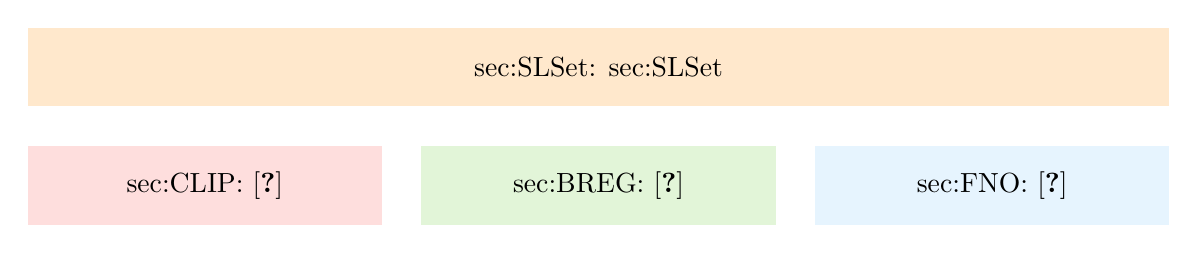
\begin{tikzpicture}
%
\hypersetup{linkcolor=black}%
\filldraw[fill=orong!20, draw=none] (0,12.5) rectangle (14.5,11.5) node[midway] {%
\cref{sec:SLSet}: \nameref{sec:SLSet}};
\filldraw[fill=grape!20, draw=none] (0,11) rectangle (4.5,10) node[midway] {\cref{sec:CLIP}: \cite{bungert2021clip}}; %
%
\filldraw[fill=apple!20, draw=none] (5,11) rectangle (9.5,10) 
node[midway] {\cref{sec:BREG}: \cite{bungert2022bregman}}; %
%
%
\filldraw[fill=sky!20, draw=none] (10,11) rectangle (14.5, 10) node[midway] {%
\cref{sec:FNO}: \cite{kabri2023resolution}};
%
\end{tikzpicture}
\end{center}
%
%
Therefore, conceptually we again highlight the keyword \textbf{sparsity} and additionally \textbf{robustness}. In \cite{bungert2021clip} we consider input robustness under adversarial perturbations. Here, the input is typically \emph{attacked} on purpose to confuse a neural network and therefore worsen its performance. In order to obtain a neural network that is less vulnerable against such attacks we propose an optimization strategy that selects parameters that yield a more robust network. In \cref{sec:CLIP} we comment on the topic and the contribution in more detail. 

A different kind of input robustness is considered in \cite{kabri2023resolution}. In the setting of image classification, images are modeled as functions on a continuum domain that need to be discretized in order to represent the on a machine. This discretization however, is usually arbitrary and not inherent to the object of interest. Therefore, it is natural to assume that the output of the network should be independent of this discretization, also referred to as resolution, for which we consider robustness w.r.t. resolution changes. We remark on this and the publication in \cref{sec:FNO}.

Concerning computational performance and memory storage of the neural network we focus on sparsity of the parameters $\param\in\Param$. In \cite{bungert2022bregman} we propose a sparse optimization strategy based on Bregman iterations, which employs $L^1$ type penalities to promote sparsity. The conceptual difference between the existing algorithm and our proposal is the stochastic computation of the gradient. Our theoretical results prove decay in loss and convergence of the iterates. Finally we also conduct numerical experiments that demonstrate the efficiency of the method. We refer to \cref{sec:BREG} for a detailed explanation.

Before, we start with the exposition on the mentioned works, we briefly review the common supervised learning framework. Building upon the basic observations in \cref{ch:SL} we give a slightly more detailed introduction in \cref{sec:SLSet}.






\section{Setting}\label{sec:SLSet}
%
We are given a finite training set $\tset\subset\Inp\times\OutSpace$. For a family of functions $f_\param:\Inp\to\OutSpace$ parameterized by $\param\in \Param$. We consider the empirical  minimization
%
\begin{align*}
\min_{\param\in\param} \empLoss(\param) 
\end{align*} 
%
where for a function $\ell:\OutSpace\times\OutSpace\to\R$ we define
\begin{align}\label{eq:empLoss}
\empLoss(\param)  := \frac{1}{\abs{\tset}}\sum_{(x,y)\in \tset} \ell(f_\param(x), y).
\end{align}
%
%
\begin{remark}{}{}
%
Assuming that $\tset$ is sampled from a joint distribution $P_{\Inp,\Oup}$ on $\Inp\times\Oup$ this approximates the computational infeasible population risk minimization
%
\begin{align*}
\int_{\Inp\times\OutSpace} \ell(f_\param(x), y) d\pi(x,y).
\end{align*}
\end{remark}
%
%
\noindent%
In the following we provide two important choices for the function $\ell:\Oup\times\Oup\to\R$.
%
%
\begin{example}{MLE}{}
For image denoising problems, we often choose $\Inp=\Oup=[0,1]^{N\times M}$ assuming only one color channel for simplicity. In this context the Mean squared $L^2$ Error (MLE), defined as
%
\begin{align*}
\ell(\oupp,\oup) := \frac{1}{N\cdot M} \norm{\oupp-\oup}^2
\end{align*}
%
is commonly employed. This loss function could however also be employed for classification problems.
\end{example}
%
%
\begin{example}{Cross-Entropy}{}
For classification problems the function $\ell:\Oup\times\Oup\to\R$ is often chosen as the \emph{cross-entropy} or \emph{negative log-likelihood} loss, \cite{good1952rational}. For two discrete probability distributions, $p,q:\{1,\ldots,C\}\to\R$ one defines
%
\begin{align*}
H(p,q) := -\sum_{c=1}^C p_c\cdot \log(q_c)
\end{align*}
%
see e.g. \cite{cybenko1998mathematics}. Assuming that $\Oup=\Delta^C$ this allows to choose $\ell(\oupp,\oup):=H(\oup, \oupp)$. If the network only maps to $\R^C$ one often additionally inserts a soft-max function $Q(\oup)_c:= \exp(\oup_c)/\sum_c \exp(\oup_c)$ (see \cite{boltzmann1868studien}) and then sets
%
\begin{align*}
\ell(\oupp, \oup) := H(\oup, Q(\oupp)).
\end{align*}
%
In the case, where the output is given as labels $\oup\in\{1,\ldots,C\}$ on sets
%
\begin{align*}
\ell(\oupp, \oup) := H(\oup_{\oh}, Q(\oupp)) = -\log(Q(\oupp))
\end{align*}
%
employing the one-hot notation. Namely, we define $\oh:\{1,\ldots,C\}\to\Delta^C$,
%
\begin{align*}
(\oup_{\oh})_i := \oh(\oup)_c:= \begin{cases} 1 &\text{ if } c=\oup,\\ 0&\text{ else }.\end{cases}
\end{align*}
%
\end{example}
%
%
\subsection{Network Architectures}
%
%
In this thesis we focus on feed-forward neural networks, i.e., we consider layers of the form
%
\begin{align}\label{eq:layer}
\Phi(w, W, b)(z):= wz + \sigma(Wz + b)
\end{align}
%
where $w\in\R$ models a residual connection, $W\in\R^{n\times n}$ is a weight matrix, $b\in\R^n$ a bias vector and $z\in\R^{m}$. We consider a concatenation of $L\in\N$ such layers, which then forms a neural network
%
\begin{align*}
f_\param = \Phi_L\circ\ldots\circ\Phi_1
\end{align*} 
%
with parameters $\param =((W_1,b_1,w_1)\ldots,(W_L,b_L,w_L))\in\Param$ and layers $\Phi^i := \Phi(w_i, W_i, b_i)$.
%
\paragraph{MLP} In the easiest case we consider a perceptron \cite{rosenblatt1958perceptron}, which models a fully connected layer, i.e. every entry $W_{ij}$ of th weight matrix is an parameter that is optimized in the training process.

\paragraph{Convolutions}\label{sec:convlayer} Especially important for visual tasks are convolutional layers. Here, we take a kernel $k\in \R^{M\times M}$ and define the application of $W=W(k)$ as
%
\begin{align*}
Wz = k\ast z
\end{align*}
%
where we refer to \cref{sec:FNO} for the concrete definition of the convolution. Typically the input is of the form $z\in\R^{K:{\text{in}}\times N \times M}$, where $K_{\text{in}}$ denotes the number of input channels. The layer is then a mapping $\Phi:\R^{K:{\text{in}}\times N \times M}\to\R^{K:{\text{out}}\times N \times M}$, where $K_{\text{out}}$ denotes the number of output channels, which can be realized by different kernels $k_{ij}$ and
%
\begin{align*}
(Wz)_{j,:,:} := \sum_{i=1}^{K_{\text{in}}} k_{ij}\ast z.
\end{align*}

\paragraph{ResNets} Often we also consider a residual component as displayed in \cref{eq:layer} with the term $wx$. The idea of adding this component was first introduced in \cite{srivastava2015highway} with a learnable parameter $w\in\R$ and later popularized in \cite{he2016deep} by fixing $w=1$, see also \cite{he2016identity}, which then yields the celebrated ResNet architecture. In the following applications we both consider the case where $w=1$ is fixed, but also the possibility of learning the parameter $w\in\R$ in \cite{bungert2021neural}.
%
\subsection{Gradient Computation and Stochastic Gradient Descent}\label{sec:SGD}
%
%
Training a neural network requires to solve a optimization problem w.r.t. to the parameters $\param\in\Param$. In this work we only focus on first order methods, however both zero \cite{riedl2022leveraging, pinnau2017consensus, carrillo2021consensus, martens2010deep} and second order methods \cite{martens2010deep} have been successfully applied in this context. Employing first order methods, requires to evaluate the gradient $\nabla_\theta \empLoss$, however in this scenario it is not common to compute the full gradient but rather to have a gradient estimator. This estimator is usually obtained by randomly dividing the train set $\trSet$ into disjoint minibatches $B_1\cup\ldots\cup B_b = \trSet$ and then successively computing the gradient of the minibatch loss
%
\begin{align*}
\empLoss(\param;B):=\frac{1}{\abs{B_i}}\sum_{(x,y)\in B_i} \ell(f_\param(x), y).
\end{align*}
%
%
Iterating over all batches $i=1,\ldots,b$ is referred to as one epoch. From a mathematical point of view this yields stochastic optimization methods, since in each step the true gradient is replaced by an estimator. In the abstract setting we let $(\Omega,F,\P)$ be a probability space and consider a function $g:\Param\times \Omega\to \Param$ as an unbiased estimator of $\nabla\empLoss$, i.e.
%
\begin{align*}
\Exp{g(\param;\omega)} = \nabla\empLoss(\param)\text{ for all } \param\in\Param.
\end{align*}
%
Most notably this method transforms the standard gradient descent update \cite{cauchy1847methode}
%
\begin{align*}
\param^{(k+1)} = \param^{(k)} - \tau^{(k)} \nabla \empLoss(\theta^{(k)})
\end{align*}
%
to \emph{stochastic} gradient descent \cite{robbins1951stochastic}
%
\begin{align*}
\text{draw }&\omega^{(k)}\text{ from }\Omega\text{ using the law of }\P,\\
g^{(k)} &:= {g(\param^{(k)};\omega^{(k)})},\\
\param^{(k+1)} &:= \param^{(k)} - \tau^{(k)} g^{(k)}.
\end{align*}
%
%
%
%
%
\clearpage%
\section{Adversarial Stability via Lipschitz Training: \cite{bungert2021clip}}\label{sec:CLIP}
%
\begin{wrapfigure}{r}{.5\textwidth}
	\centering
	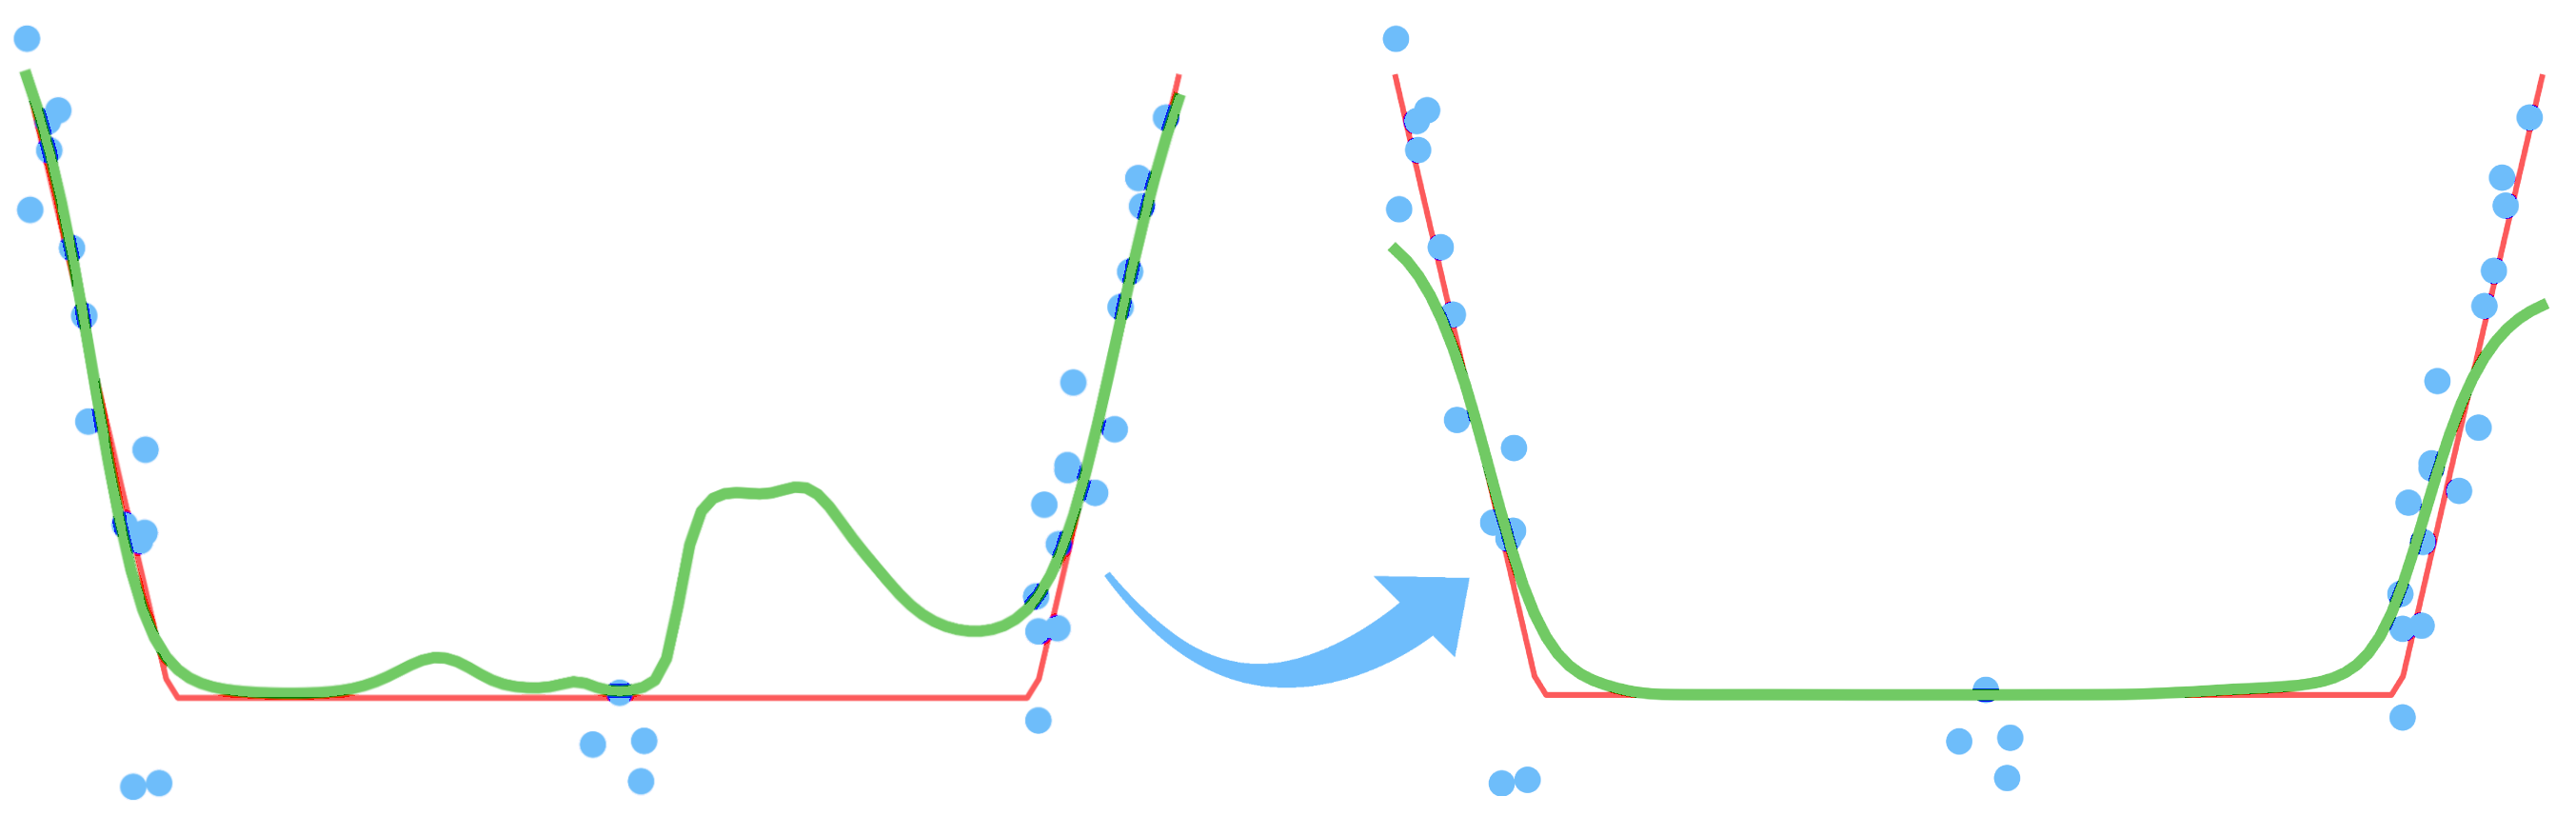
\includegraphics[width=.5\textwidth]{atelier/CLIP/CLIP.png}
\end{wrapfigure}
%
%
In the following we consider classification problems with $C\in\N$ different classes and functions $\net:\Inp\to\Delta^C$ for which we denote by 
\begin{align*}
\net^\MAP(\inp):=\argmax_c \net(\inp)_c
\end{align*}%
%
the maximum a posteriori estimation for input $\inp\in\Inp$. The capabilities of neural networks to perform classification tasks on unseen data---i.e. inputs $x\in\Inp$ that are not part of the training data---are impressive and the reason for their popularity. However, it has been noticed in \cite{goodfellow2014explaining} that is relatively easy to \enquote{fool} classification networks in the following sense:
%
\begin{center}
\textit{
Given a classification network and a human classifier $f_\param, h:\Inp\to\Delta^C$, and an input $\inp\in\Inp$ such that $f_\param^\MAP(\inp) = h^\MAP(\inp)$. An adversarial example is an input $\inpp\in \Inp$ that is close to $\inp$ and
%
\begin{align*}
f_\param(\inpp)\neq h(\inpp) = h(\inp).
\end{align*}
}
\end{center}
%
%
The vague concept of a \emph{human classifier}, incorporates the intuition of the classification problem as a human would solve it. Assuming that we are given data $\tset\subset \Inp\times\Oup$ that is samples i.i.d. from a joint distribution $P_{\Inp,\Oup}$ this function could also be chosen as $h(x)_c:=P_{\Inp,\Oup}(c|\inp)$.


\begin{remark}{}{}
While we mostly focus on neural networks, some authors argue that these instabilities are inherent to certain classification problems \cite{shafahi2018adversarial, fawzi2018adversarial}. From this point of view, trying to defend against these instabilities is not necessarily desirable.
\end{remark}
%
%
%
\paragraph{What are Adversarial Examples Formally?} In order to formalize this idea we omit any influence of the typically unavailable function $h$ and instead consider $\inpp$ adversarial if $\net_\param(\inp)\neq\net_\param(\inpp)$, i.e. we assume $\net_\param(\inp)$ to be \enquote{correct}. Furthermore, in this work we assume that $\Inp$ models an image space $\Inp=\R^{K\times N\times M}$, with $K,N,M\in\N$ and choose a distance $d:\Inp\times\Inp\to\R^+_0$ to measure the distance between points in $\Inp$. 
%
\begin{remark}{}{}
In most of our examples we choose $d(\cdot,\cdot) = \norm{\cdot - \cdot}_p$. Employing a $L^p$ norm in an image context---via pixel-wise comparison---can be an unfavorable choice. Images that appear very different visually, (i.e. for a human classifier) can have a smaller $L^p$ distance, than images that visually appear similar, see e.g. \cite[Fig. 16]{stanczuk2021wasserstein}. However, it is easy to evaluate, which is crucial for most applications. In the absence of a better criterion, having a small $L^p$ norm, is commonly the only way to decide if $\inpp$ is an admissible adversarial example. 
\end{remark}
%
%
\noindent%
Employing these simplifications we then say that $\inpp\in\Inp$ is adversarial, if
%
\begin{align*}
d(\inp,\inpp) \leq \budget \qquad \text{ and } \qquad \net_\param(\inp)\neq \net_\param(\inpp),
\end{align*}
%
where $\budget$ is called the \emph{adversarial budget}. This parameter controls how far $\tilde{x}$ can be from the original point $x$ to be still considered adversarial. Here, we also have decide how much we trust the metric $d(\cdot,\cdot)$ as a measure of closeness. This interpretation only makes sense, if we assume that $\net_\param(\inp)$ is \emph{correct}, which can only be easily checked on the training data \cite{bungert2023begins}.
%
%
\paragraph{Types of Adversarial Examples} Typically, adversarial examples are created from the clean image $\inp$ via some distortion $\delta\in\R^n$. Together with an application map $T:\Inp\times\R^s\to\Inp$ one then obtains $\inpp=T(x,\delta)$ as the adversarial example. In this formulation one can the alternatively employ the criterion $\norm{\delta}\leq \budget$ to decide, whether $T(\inp,\delta)$ is an adversarial example. We only list some of the approaches below:
%
\begin{itemize}
\item\textbf{Addition}: the most well-known examples are created by $T(x,\delta):=\inp+\delta$, i.e. $\inpp = \inp + \delta$. Here, it is important to note that typically images are assumed to have values between $0$ and $1$, i.e. $\Inp=[0,1]^{K\times N\times M}$ for which it is important to ensure that $\inpp\in\Inp$.
%
\item\textbf{Translation and Rotation}: Simple geometric transformations---that would be unnoticeable for a human classifier---are quite effective to \enquote{fool} neural networks. Employing translations $T_{\text{t}}:\Inp\times\Inp\to\Inp$ one has to choose the behavior on the boundary such that one obtains a valid image. The same holds true for rotations $T_{\text{r}}:\Inp\times [-\pi,\pi]\to\Inp$. In this case $\delta\in[-\pi,\pi]$ models the angle of the rotation and would yield an admissible adversarial example, if $\abs{\delta}\leq \budget$. Here, we see that this formulation looses some expressivity. Consider the MNIST dataset \cite{leCun10}, where the task is to classify handwritten digits from $0$ to $9$:
%
\begin{itemize}
\item We see that only $\budget<\pi/2$ makes sense, otherwise the number \enquote{6} could be always transformed to the number \enquote{9} and vice versa.
\item However, considering the number \enquote{0} rotations above the angle $\pi/2$ can definitely yield proper adversarial examples $\inpp$.
\end{itemize}
%
We refer to \cite{engstrom2018rotation} for a study on these types of adversarial examples.
%
\item\textbf{Change of Basis}: As explored in \cite{guo2017countering} one can consider a different orthonormal basis of the image space $\R^{K\times N\times M}$ and then perform the attack w.r.t. this basis. 
The transform $T:\Inp\times\R^{K\times N\times M}\to\Inp$ first obtains the different representation of $\inp$, then adds the coefficients of $\delta$ and then maps back to the original basis. This is only meaningful, if one restricts certain coefficients of $\delta$ to be zero in the alternative basis. For example, the discrete cosine transform (\cite{ahmed1974discrete}) has been applied successfully in this context \cite{guo2017countering}.
\end{itemize}
%
%
In the following we restrict ourselves to the additive case and only consider examples $\inpp = \inp + \delta$.
%
%
\paragraph{Finding Adversarial Examples} Employing a loss function $\ell:\Oup\times\Oup\to\R$ the task of finding an adversarial examples $\inpp=\inp+\delta\in\Inp$ can be relaxed via solving the problem
%
\begin{align}\label{eq:advprob}
\max_{\inpp\in \Inp:d(\inp,\inpp)\leq \budget} \ell(\oup, \net_\param(\inpp))
=
\max_{\delta:\norm{\delta}_d\leq\delta, \inp+\delta\in\Inp}
\ell(\oup, \net_\param(\inp+\delta),
\end{align}
%
where $\oup=\net_\param(\inp)$. Solving this problem is referred to as \emph{attacking} the network $\net$. More precisely, this is a so-called \emph{untargeted} attacks, since we do not prescribe $\inpp$ to realize any special output as long as it confuses the network. Opposed to this, there are so called \emph{targeted} attacks. Here we pick $c^\adv \neq \net^\MAP_\param(\inp)$ and then want to find $\inpp$ such that $\net^\MAP_\param(\inpp) = c^\adv$. Here, we then consider the problem
%
\begin{align*}
\min_{\inpp\in \Inp:d(\inp,\inpp)\leq \budget} \ell(c^\adv_{\oh}, \net_\param(\inpp)).
\end{align*}
%
%
However, we see that conceptually this problem is similar to \cref{eq:advprob} and differs only by a change of sign and a different reference label.
%
A popular method to solve \cref{eq:advprob} is the projected sign gradient ascent iteration \cite{kurakin2016adversarial},
%
\begin{align*}
\inpp^\k{k+1} = \operatorname{Proj}_d(\inpp^\k{k} + \tau \sign(\nabla_{\inpp}
\ell(\net_\param(\inp), \net_\param(\inpp^\k{k})))).
\end{align*}
%
%
%
Here, $\operatorname{Proj}_d$ denotes the projection onto the set $\Inp\cap B_{d,\budget}(\inp)$, where $B_{d,\budget}(\inp)$ is the ball with radius $\budget$ around $\inp$, w.r.t. to the distance $d$. Performing only one step of this iteration yields the fast gradient sign method \cite{goodfellow2014explaining}. There is a wide variety of these so-called gradient-based white-box attacks \cite{yuan2019adversarial}, i.e. methods that assume that the gradient of the model is available. In more realistic scenarios, this might not be the case. Attacks that do not employ the actual gradient of the model to attack are called \emph{black box} attacks \cite{ilyas2018black}, which however not part of this thesis.
%
%
\paragraph{Defending against Adversarial Attacks}
%
%
We consider the question of finding parameters $\param\in\Param$ such that corresponding model $\net_\param$ is \emph{adversarially robust}, i.e. is less vulnerable to attacks. Therefore, we want the attack problem in \cref{eq:advprob} to be hard to solve. This intuition leads to the optimization problem
%
\begin{align*}
\min_{\param\in\Param} \sum_{(\inp,\oup)\in \tset} \max_{\inpp\in B_{d,\budget}(\inp)} \ell(\net_\param(\inpp), \oup)
\end{align*}
%
which is known as the \emph{adversarial training} formulation \cite{kurakin2016adversarial2, madry2017towards}. From a distributionally robust optimization point of view, this problem relates to 
%
\begin{align*}
\min_{\param\in\Param} \max_{\tilde P: D(P_{\Inp,\Oup}, \tilde P)\leq\budget} \int_{\Inp\times\Oup} \ell(\net_\param(\inp), \oup)\ d\tilde{P}(\inp,\oup)
\end{align*}
%
where $D$ denotes some distance on probability distributions, see \cite{bungert2023geometry}. Employing a batched gradient descent type iteration, one then has to solve a problem of the form \Cref{eq:advprob} in every step, which can be interpreted as a form of data augmentation \cite{lecun1995learning}. 
%
%
%
\paragraph{Lipschitz Training of Neural Networks}
%
Adversarial robustness is closely related to the Lipschitzness of a network $\net_\param$. Namely, for inputs $\inp,\inpp\in\Inp$ that are close, we also want the outputs of $\net_\param$ to be close. In other words we want to find a small constant $L>0$ such that
%
\begin{align*}
\norm{\net_\param(\inp) - \net_\param(\inpp)}_\Oup \leq L\ \norm{\inp-\inpp}_\Inp,
\end{align*}
%
where we typically employ an $L^p$ norm both $\norm{\cdot}_\Inp$ and $\norm{\cdot}_\Oup$.
%
The smallest constant fulfilling this inequality is the Lipschitz constant $\Lip(\net_\param)$. Having some control over this constant can therefore relate to being adversarially robust.
%
\begin{remark}{}{}
Apart from adversarial robustness, having an upper bound on the Lipschitz constant of a neural network is also important for other applications, see e.g. \cite{hasannasab2020parseval, arjovsky2017wasserstein}.
\end{remark}
%
%
We employ the Lipschitz constant as a regularizer and consider the problem
%
\begin{align}\label{eq:LipReg}
\min_\param \empLoss(\param) +\lambda\ \Lip(\net_\param)
\end{align}
%
for a parameter $\lambda$. Unfortunately, computing the Lipschitz constant of neural networks is a NP-hard problem \cite{scaman2018lipschitz}, therefore many works employ the estimate
%
\begin{align}\label{ineq:lip_weights}
\lip(\net_\param) \ \leq \ \prod_{l=1}^L  \lip(\Phi_l) \leq 
C_\sigma \prod_{l=1}^L \norm{W_l},
\end{align}
%
where here $\norm{W_l}$ denotes some matrix norm and $C_\sigma$ depends on the Lipschitz constants of the activation functions, see \cite{Anil2019,gouk2020regularisation, Krishnan2020, Roth2020}.
%
This inequality is not sharp and usually overestimates the Lipschitz constant, as we see in the following example taken from \cite{bungert2021clip}.
%
\begin{example}{}{}
We consider a feed-forward neural network $\net_\param:\R\to\R$ with one hidden layer,
%
\begin{align*}
\Phi_1(z) &:= \relu(W_1 z) :=\left(\max\{z, 0\}, \max\{-z, 0\}\right)^T,\qquad 
W_1:= (1,-1),\\
\Phi_2(z) &:= W_2 z := z_1 + z_2,\qquad W_2:=(1,1)^T,\\
\net_\param&:= \Phi_2\circ\Phi_1.
\end{align*}
%
For $\inp\in\R$ we have that 
%
\begin{align*}
\inp&\geq 0 \qquad\Rightarrow\Phi_1(\inp) = (\inp, 0)^T \qquad\Rightarrow \net_\param(\inp)=\inp,\\
\inp&\leq 0 \qquad\Rightarrow\Phi_1(\inp) = (0, -\inp)^T \qquad\Rightarrow \net_\param(\inp)=-\inp,
\end{align*}
%
and therefore $\net_\param = \abs{\cdot}$, for which we know that $\Lip(\net_\param)=1$. However employing the spectral for $W_1$ and $W_2$, we see that
%
\begin{align*}
\norm{W_1}\cdot\norm{W_2} = \sqrt{2}\ \sqrt{2} = 2.	
\end{align*}
%
\end{example}
%
Plugging the estimate of \cref{ineq:lip_weights} into \cref{eq:LipReg} therefore potentially over regularizes the problem.
%
\paragraph{Contribution in \cite{bungert2021clip}} In \cite{bungert2021clip} we propose a strategy to solve \cref{eq:LipReg} approximately, without the estimate in \cref{ineq:lip_weights}. The basic idea consists of approximating the Lipschitz constant on a finite set and using this approximation as a regularizer. Furthermore, we analyse the original model in \cref{eq:LipReg} where we study existence of solutions, the influence of the parameter $\lambda$ and the limits $\lambda\to 0, \lambda\to \infty$, see \cref{sec:CLIPAna}. Finally, we demonstrate the efficiency of the methods by applying to some simple toy problems, see \cref{sec:CLIPNum}.


\subsection{Cheap Lipschitz Training}
As mentioned before, we approximate the Lipschitz constant on a finite set $\Inp_{\lip{}}\subset\Inp\times\Inp$ via
%
\begin{align*}
\Lip(\net_\param; \Inp_{\lip{}}) := 
\max_{(\inp,\inpp)\in\Inp_{\lip{}}} \frac{\norm{\net_\param(\inp)-\net_\param(\inpp)}_\Oup}{\norm{\inp-\inpp}_\Inp}
\approx
\Lip(\net_\param).
\end{align*}
%
%
Disregarding the non-differentiable points of $\param\mapsto \Lip(\net_\param; \Inp_{\lip{}})$ allows us to make the above approximation in \cref{eq:LipReg} and the solve then problem via a gradient descent variant.
%
\begin{remark}{}{}
Let $f,g:\Inp\to\Oup$ be two differentiable functions. If $f(\inpp)>g(\inpp)$ for some $\inpp\in\Inp$ then we know that there exists some $\epsilon>0$ such that $f(\inp)>g(\inp)\forall \inp\in B_\epsilon(\inpp)$. We have that $f\vee g = \max\{f,g\} = f$ in $B_\epsilon(\inpp)$ and therefore $\inp\mapsto f(\inp)\vee g(\inp)$ is differentiable in $\inpp$. If $f(\inpp)=g(\inpp)$ then $f\vee g$ could be non-differentiable at $\inpp$. However, in practice we employ automatic differentiation, where in this case one of the functions is chosen, say $f$, and the \emph{gradient} at $\inpp$ is computed as $\nabla f$. 
\end{remark}
%
%
\noindent%
The strength of this approach of course is dependent on the quality of the set $\Inp_{\lip}$. In \cite{bungert2021clip} we propose to iteratively update the set via a gradient ascent type scheme. Namely, we initialize $\Inp_{\lip}$ as a random perturbation of a subset of the given data. In each step we then update the points as follows:
\begin{itemize}
\item Consider $L(\inp,\inpp) := {\norm{\net_\param(\inp)-\net_\param(\inpp)}}\,/\,{\norm{\inp-\inpp}},\quad\inp,\inpp\in\Inp$.
\item For each $(\inp,\inpp)\in\Inp_{\lip}$ perform the update 
%
\begin{align*}
\inp\phantom{'} &\gets \inp\phantom{'} + \tau\,L(\inp,\inpp) \nabla_{\inp} L(\inp,\inpp),\\
\inpp &\gets \inpp + \tau\,L(\inp,\inpp) \nabla_{\inpp} L(\inp,\inpp),
\end{align*}
%
for a parameter $\tau>0$.
\end{itemize}
%
This scheme performs a gradient ascent on the Lipschitz constant, see \cite[Alg. 1]{bungert2021clip}. For each mini batch $B\subset\tset$ we first update the set $\Inp_{\lip}$ and then update the parameters via
%
\begin{align*}
\param \gets \param - \eta\ \nabla_\param\left(\empLoss(\param; B) + 
\lambda~\Lip(\net_\param,\Inp_{\lip})\right)
\end{align*}
%
which yields the algorithm presented in \cite[Alg. 2]{bungert2021clip}. Similar to \cite{shafahi2019adversarial} one can reuse the gradients computed for $\nabla_\inp$ for the computation of $\nabla_\param$. This fact yields the attribute \emph{cheap} in the Lipschitz training algorithm.
%
\subsection{Analysis of Lipschitz Regularization}\label{sec:CLIPAna}
%
In \cite{bungert2021clip} we analyse some basic properties of the original regularization problem in \cref{eq:LipReg}. We repeat the assumptions we made therein, in order to refer to them in the following.

\begin{enumerate}[label= \textbf{Assumption \arabic*.}, ref={\arabic*}, align=left]
	\setlength{\itemsep}{9pt}
	\item\label[assumption]{ass:closs} We assume that the loss function 
	$\loss:\Oup\times\Oup\to\R\cup\{\infty\}$ satisfies:\\[-0.2cm]
	\begin{enumerate}
		\setlength{\itemsep}{6pt}
		\item $\loss(\oup,\oupp)\geq 0$ for all $\oup,\oupp\in\Oup$,
		\item $\oup\mapsto\loss(\oup,\oupp)$ is lower semi-continuous for all $\oupp\in\Oup$.
	\end{enumerate}
	% ###
	\item\label[assumption]{ass:net} We assume that the map $\param\mapsto\net_\param(\inp)$ 
	is continuous for all $\inp\in\Inp$.
	% ###
	\item\label[assumption]{ass:exist} We assume that there exists $\param\in\Param$ such that 
	\begin{align*}
		\frac{1}{\abs{\trSet}}
		\sum_{(\inp,\oup)\in\trSet}\loss(\net_\param(\inp),\oup)+
		\lambda \lip(\net_\param) < \infty.
	\end{align*}
\end{enumerate}
%
%
Employing only \cref{ass:net} one can show that that the map $\param\mapsto \Lip(\net_\param)$ is lower semi-continuous, \cite[Lem. 1]{bungert2021clip}. 
%
\paragraph{Existence} If $\Param$ is compact or finite, one can show that there exist solutions of \labelcref{eq:LipReg}. In the general case one needs to add a norm term, that ensures boundedness of a minimizing sequence. The following is the main existence result, which can be proven by the direct method in the calculus of variations \cite{dacorogna2007direct}.
%
\begin{proposition}{\cite[Prop. 1]{bungert2021clip}}{}
Under \cref{ass:closs,ass:net,ass:exist} the problem
\begin{align*}
\min_{\param\in\Param}
\frac{1}{\abs{\trSet}}
\sum_{(\inp,\oup)\in\trSet}
\loss(\net_\param(\inp),\oup) + 
\lambda\lip(\net_\param) + \mu\norm{\param}_\Param
\end{align*}
has a solution for all values $\lambda,\mu>0$.
Here, $\norm{\cdot}_\Param$ denotes a norm on $\Param$.
\end{proposition}
%
%
\paragraph{Dependency on the Regularization Parameter} Assuming that for every $\lambda>0$ we have a solution $\param_\lambda\in\Param$ of \cref{eq:LipReg} one can show that
%
\begin{alignat*}{2}
\lambda&\longmapsto
\frac{1}{\abs{\trSet}}
\sum_{(\inp,\oup)\in\trSet}\loss(\net_{\param_\lambda}(\inp),\oup) \quad&&\text{is non-decreasing,}
\\
\lambda&\longmapsto\lip(\net_{\param_{\lambda}}) 
\quad&&\text{is non-increasing.}
\end{alignat*}
%
%
This statement is the content of \cite[Prop. 2]{bungert2021clip}, however, the argument is exactly the same as in \cite{burger2013guide}. The intuition behind this result is that with increasing parameter $\lambda$ solutions of \cref{eq:LipReg}---more precisely the corresponding networks---have smaller Lipschitz constants, i.e. tend to be more constant, which however also diminishes their expressivity. We formalize the limit cases in the following.

Assuming the realizability condition of \cite{shalev2014understanding} we know that there exists parameters $\param\in\Param$ such that $\empLoss(\theta)=0$. This means there are parameters that fit the data perfectly. Considering the limit $\lambda\to 0$ we obtain convergence to a solution of the unregularized problem with the smallest Lipschitz constant.
%
\begin{proposition}{\cite[Prop. 3]{bungert2021clip}}{}
Let \cref{ass:closs,ass:net,ass:exist} and the realizability assumption~\cite{shalev2014understanding} be satisfied. If $\param_\lambda \to \param^\dagger\in\Param$ as $\lambda\searrow 0$, 
then
%
\begin{align*}
\param^\dagger\in\argmin\left\lbrace \lip(\net_\param) \st \param\in\Param,\, \frac{1}{\abs{\trSet}}
\sum_{(\inp,\oup)\in\trSet}\loss(\net_{\param}(\inp),\oup)
=0\right\rbrace
\end{align*}
%
if this problem admits a solution with $\lip(\net_\param)<\infty$.
\end{proposition}
%
%
\noindent%
Furthermore, we study the effect of sending $\lambda\to\infty$, where we see that the network $\net_{\param_\lambda}$ indeed tends to be constant as expected. We can explicitly characterize this constant as the closest point to barycenter of the output data, that is realizable by a neural network. 
%
\begin{proposition}{\cite[Prop. 4]{bungert2021clip}}{}
Let \cref{ass:closs,ass:net,ass:exist} be satisfied and assume that 
\begin{align*}
\mathcal{M}:=
\left\{\oup\in\Oup \st \exists\param\in\Param,\,
\net_\param(\inp)=y,\,\forall\inp\in\Inp\right\}\neq\emptyset.
\end{align*}
%
If $\param_\lambda \to \param_\infty \in\Param$ as $\lambda\to \infty$, then $\net_{\param_\infty}(\inp)=\hat{\oup}$ for all $\inp\in\Inp$ where 
\begin{align*}
\hat{\oup}\in\argmin_{\oup'\in\mathcal{M}}
\frac{1}{\abs{\trSet}}
\sum_{\oup\in\trSetY}\loss(\oup',\oup).
\end{align*}
\end{proposition} 
%
%
\clearpage%
\subsection{Numerical Results}\label{sec:CLIPNum}
%
 
\begin{wrapfigure}{r}{.4\textwidth}
\begin{center}

\includegraphics[width=.4\textwidth]{atelier/CLIP/CLIPQR.png}
\end{center}
The code for all the experiments is available at \href{https://github.com/TimRoith/CLIP}{github.com/TimRoith/}\\
\href{https://github.com/TimRoith/CLIP}{CLIP}.
\end{wrapfigure}
We briefly comment on the numerical results \cite{bungert2021clip}. All the experiments were implemented in \texttt{Python} \cite{van1995python} employing---among others---the \texttt{PyTorch} \cite{paszke2019pytorch} package. We conduct experiments on the MNIST \cite{leCun10} and FashionMNIST \cite{Han17} datasets.

\paragraph{Qualitative Example} We first apply the CLIP scheme to regularize a one-dimensional regression problem. In Fig.2 therein, one observes can observe qualitatively the effect of the regularization. Namely, we are given noisy data from a ground truth function for which the unregularized problem tend to overfit the data. The resulting network has fluctuations and therefore a large Lipschitz constant in certain regions, where the ground truth function has a small Lipschitz constant. With increasing parameter $\lambda$ we observe that the networks $f_{\param_\lambda}$ are smoothed out and better approximate the ground truth function.
%
\paragraph{Quantitative Evaluation of Adversarial Robustness} We additionally evaluate how robust a CLIP trained network is against adversarial attacks. Next to a standard learning rate scheduler, we also update the regularization parameter $\lambda$ throughout the training process. Namely, we choose a target accuracy be and evaluate the loss on a validation set after the epoch. If this accuracy is less then the target we decrease $\lambda$ and increase it if the accuracy is higher. In Table 1 of \cite{bungert2021clip} we compare ourselves against a weight regularization scheme that is based on the estimate in \cref{ineq:lip_weights}. We see that CLIP outperforms this method in most cases.
%
%
%
%
%
%
%
%
\clearpage%
\section{Sparsity via Bregman Iterations: \cite{bungert2022bregman}}\label{sec:BREG}
%
\begin{wrapfigure}{r}{.5\textwidth}
\centering
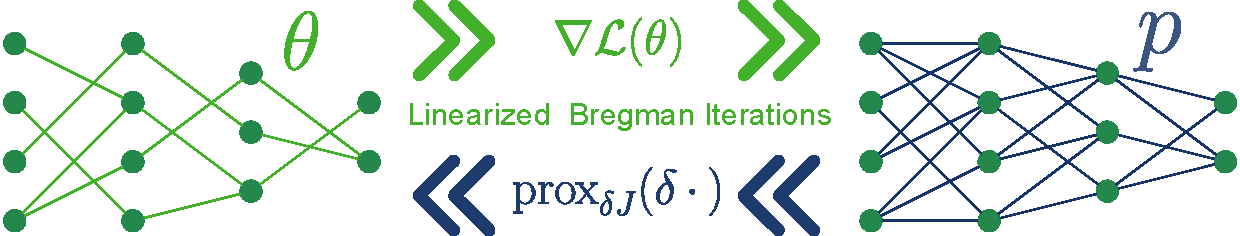
\includegraphics[width=.5\textwidth]{atelier/Breg_dist/BregmanPosterCartoon.pdf}
\end{wrapfigure}
%
%
Starting from the first simple neural architectures (e.g. \cite{rosenblatt1958perceptron}) the size of typical architectures has grown significantly in the last years \cite{hoefler2021sparsity}. While this development allowed to solve increasingly difficult tasks with neural networks, it also lead to immense computational requirements, both for the training and evaluation of the net. Therefore, the question arises how the evaluation and training of large neural networks can be made more efficient. Some of the approaches here include (see \cite{gholami2021survey} for a comprehensive overview):
%
\begin{itemize}
\item \textbf{Architecture Optimization}: Designing an architecture that can be trained to have the same performance as a comparable one, while having less parameters, e.g. \cite{elsken2019neural, howard2017mobilenets}.
%
\item \textbf{Quantization}: Lowering the precision of the machine numbers of the parameters, e.g. \cite{banner2018scalable, courbariaux2014training}.
%
\item \textbf{Knowledge distillation}: Employing a trained larger network to learn a smaller network in a student-teacher approach, e.g. \cite{schmidhuber1992learning, hinton2015distilling}.
%
\item \textbf{Pruning}: Parameters with small saliency, i.e., parameters that contribute little to the effective output of the network are removed or set to zero, in order to obtain a sparse weight matrix or a smaller architecture, see e.g. \cite{lecun1989optimal, hassibi1993optimal}.
\end{itemize}
%
%
From the above methods, the pruning approach is most influential to our work in \cite{bungert2022bregman}. Namely, the concept of compressing the neural network by sparsifying the weight matrices is similarly employed. However, there are a few deviations from the classical pruning framework, which we remark in the following.

\paragraph{Sparsity via Optimization} In \cite{lecun1989optimal, hassibi1993optimal} one assumes to be given a trained neural network, which is then compressed after training based on some criterion. The authors in \cite{castellano1997iterative} employ an iterative pruning scheme, where a similar criterion is employed in order to throw away certain network weights after each step. In our work we want to employ a $L^1$ type penalty on weight matrices $W\in\R^{n\times m}$,
%
\begin{align*}
\norm{W}_1 = \sum_{i=1}^n\sum_{j=1}^m \abs{W_{ij}}
\end{align*}
%
which has been widely employed to obtain sparse solution, e.g. \cite{claerbout1973robust}. In \cite{tibshirani1996regression} this yields to the so-called Lasso problem
%
\begin{align*}
\min_\param \empLoss(\param) + \lambda \norm{\param}_1,\qquad \lambda >0,
\end{align*}
%
where we extend the $L^1$ norm to $\Param$ as discussed in \cref{sec:Bregnum}. This problem can for example by solved by a proximal gradient descent iteration
%
\begin{align}\label{eq:proxgd}
\param^\k{k+1} = \operatorname{soft\ shrinkage}(\param - \tau \nabla\empLoss(\param^\k{k}))
\end{align}
%
where the shrinkage operator is defined in \cref{ex:softshrink}. This iteration was employed in \cite{nitanda2014stochastic, rosasco2014convergence, reddi2016proximal} to train sparse neural networks.
%
%
\paragraph{Sparse-to-Sparse Training} All of the sparsity-based methods mentioned before start with dense weight matrices and only decrease the number of parameters during or at the end of the training process. Our approach yields an iteration, where the network is sparse throughout the iteration. In fact we start with only very few non-zero parameters and only activate necessary weights during training. This paradigm is known as sparse-to-sparse or evolutionary training \cite{mocanu2018scalable, dettmers2019sparse, Evci2020, dai2019nest, fu2019exploring, huang2016split, liu2021}.
%
%
\paragraph{Contribution in \cite{bungert2022bregman}}
%
Our work falls into the regime of sparse-to-sparse training. However, instead of relying on some heuristic growth strategy, we employ the concept of inverse scale flows (see \cref{sec:convprelim}) which allows us to obtain a optimization-driven framework, with a time-continuous interpretation. We propose a stochastic variant of linearized Bregman iterations (\cref{sec:Bregmom}) and employ it to train a sparse neural network. We show monotonic decrease of the loss in the stochastic setting---which is not possible in the case of proximal gradient descent \cref{eq:proxgd}---and convergence of the iterates under additional convexity assumptions, see \cref{sec:ConvAna}. Finally, we demonstrate the numerical efficiency of the method (see \cref{sec:Bregnum}) and provide an interesting applications for neural architecture search, which was further developed in \cite{bungert2021neural}.


\subsection{Preliminaries on Convex Analysis and Bregman Iterations}\label{sec:convprelim}

We first review some necessary concepts from convex analysis that allow us to introduce the framework in \cite{bungert2022bregman}. We refer to \cite{benning2018modern, rockafellar1997convex, bauschke2011convex} for a more exhaustive introduction to the topics.
%
The functional $\func$ is called lower semicontinuous if $\func(u)\leq\liminf_{n\to\infty}\func(u_n)$ holds for all sequences $(u_n)_{n\in\N}\subset\Param$ converging to $u$.
%
\begin{definition}{}{}
Given a Hilbert space $\Param$ and a functional $\func:\Param\to(-\infty,\infty]$.
%
\begin{enumerate}
\item The functional $\func$ is called convex, if
%
\begin{align}
    \func(\lambda\overline{\param}+(1-\lambda)\param)\leq
    \lambda\func(\overline{\param})
    +(1-\lambda)\func(\param),\quad\forall\lambda\in[0,1],\,\overline{\param},\param\in\Param.
\end{align}
%
\item The effective domain of $\func$ is defined as $\dom(\func):=\{\param\in\Param\st\func(\param)\neq\infty\}$ and $\func$ is called proper if $\dom(\func)\neq\emptyset$.
\end{enumerate} 
\end{definition}
%
%
In the following we want to consider functionals $J$ that are convex, but not necessarily differentiable. Therefor, we define the subdifferential.
%
\begin{definition}{}{}
of a convex {and proper} functional $\func:\Param\to(-\infty,\infty]$ at a point $\param\in\Param$ as
% ---------------------------------------------------------
\begin{align}
\label{eq:subgrad}
    \partial\func(\param) := \left\lbrace \sg\in\Param \st \func(\param) + \langle\sg,\overline{\param}-\param \rangle \leq \func(\overline{\param}),\;\forall\overline{\param}\in\Param\right\rbrace.
\end{align}
\end{definition}
% ---------------------------------------------------------
If $\func$ is differentiable, then the subdifferntial coincides with the classical gradient (or Fr\'echet derivative). We denote $\dom(\partial\func):=\{\param\in\Param\st\partial\func(\param)\neq\emptyset\}$ and observe that $\dom(\partial\func)\subset\dom(\func)$.

The main algorithm in this section are so-called Bregman iterations, for which we first define the Bregman distance.
%
\begin{definition}{Bregman Distance}{}
Let $\func:\Param\to(-\infty,\infty]$ be a proper, convex functional. Then we define for $\param\in\dom(\partial\func),\overline{\param}\in\Param$
% ---------------------------------------------------------
\begin{align}\label{eq:bregman_distance}
D^\sg_\func(\overline{\param},\param) := \func(\overline \param)-\func({\param})-\langle\sg,\overline\param-{\param}\rangle,\quad\sg\in\partial\func(\param).
\end{align}
%
For $\sg\in\partial\func({\param})$ and $\overline\sg\in\partial\func(\overline{\param})$ we define the \emph{symmetric} Bregman distance as
\begin{align}
D^\mathrm{sym}_\func(\overline{\param},\param) := D^\sg_\func(\overline{\param},\param) + D^{\overline{\sg}}_\func(\param,\overline\param).
\end{align}
\end{definition}
% ---------------------------------------------------------
Intuitively, the Bregman distance $D^\sg_\func(\overline{\param},\param)$, measures the distance of $\func$ to its linearization around $\param$, see \cref{fig:Bregdist}. If $J$ is differentiable, then the subdifferential is single valued---we can suppress the sup script $\sg$---and we have
%
\begin{align*}
D_J(\overline\param,\param) = \func(\overline \param)-\func({\param})-\langle\,\nabla \func(\param), \overline\param-{\param}\rangle.
\end{align*}
%
\begin{figure}
\centering
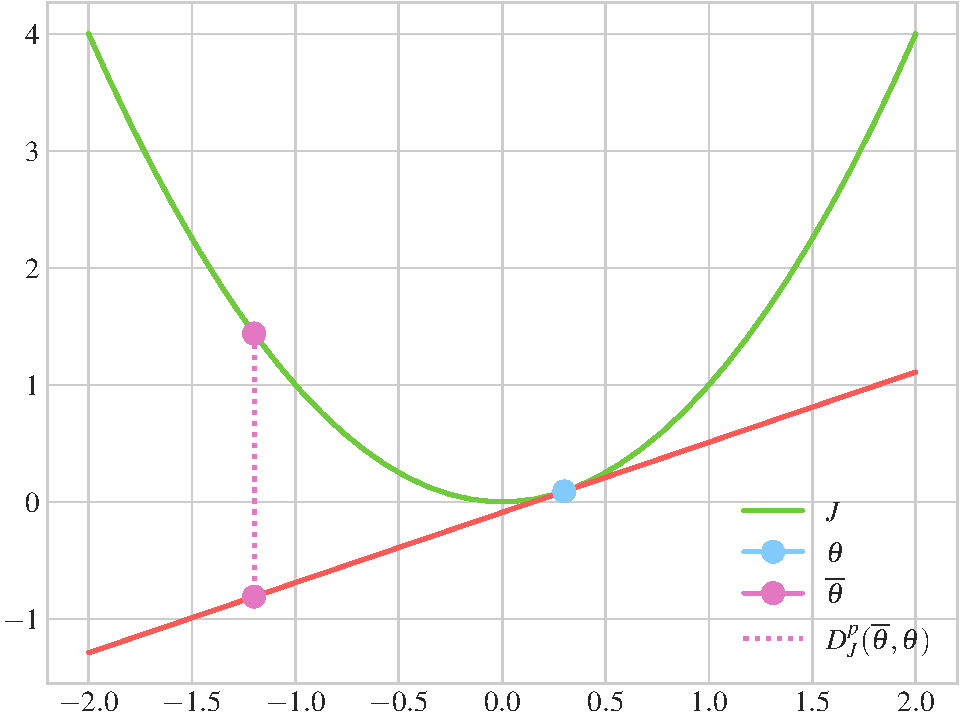
\includegraphics[width=.7\textwidth]{code/Bregman/lin_dist.pdf}
\caption{Visualization of the Bregman distance.}\label{fig:Bregdist}
\end{figure}
%
\begin{example}{}{ex:BregNorm}
For $\Param=\R^n$ and $J=\frac{1}{2}\norm{\cdot}_2^2$ we see that $\partial J(\param) = \{\param\}$ and therefore
%
\begin{align*}
D_J^p(\overline{\param}, \param) &= 
\frac{1}{2}\langle \overline\param,\overline\param\rangle - 
\frac{1}{2}\langle \param,\param\rangle - \langle \param, \overline\param-\param\rangle 
\\&=
\frac{1}{2}\langle \overline\param,\overline\param\rangle+
\frac{1}{2}\langle \param,\param\rangle -
\langle \param,\overline\param\rangle
\\&=
\frac{1}{2}\norm{\overline\param - \param}_2^2 = J(\overline\param - \param).
\end{align*}
\end{example}
%
We can easily see that in general it is neither definite, symmetric nor fulfills the triangle inequality, hence it is not a metric. 
However, it fulfills the two distance axioms
\begin{align}
D^\sg_\func(\overline{\param},\param) \geq 0,\quad D^\sg_\func(\param,\param)=0,\quad\forall\overline{\param}\in\Param,\param\in\dom(\partial\func).
\end{align}
%
The same holds for the symmetric Bregman distance, where additionally---as the name suggests---the symmetry property is fulfilled.
%
%
The last concept that is crucial in \cite{bungert2022bregman} is the so-called proximal operator.
%
\begin{definition}{}{}
Let $\func:\Param\to(-\infty,\infty]$  be convex, proper and lower semicontinuous functional, then we define the \emph{proximal operator} as
\begin{align*}
    \prox{\func}(\overline{\param}) := \argmin_{\param\in\Param} \frac{1}{2}\norm{\param-\overline{\param}}^2 + \func(\param).
\end{align*}
\end{definition}
%
If $\func$ is additionally a closed function, i.e., its sublevel sets
%
\begin{align*}
N_\alpha = \{\param\in\dom \func: \func(\param)\leq \param\}
\end{align*} 
%
are closed for every $\alpha\in\R$ then we have that the function $\tilde J = \frac{1}{2}\norm{\param -\cdot}^2 + \func(\param)$ is closed, proper and \emph{strongly} convex and therefore has a unique minimizer, see \cite[Thm. 27.1]{rockafellar1997convex}. Additionally, one often considers a regularization parameter $\lambda>0$ and is then interested in $\prox{\lambda \func}$.
%
\begin{remark}{}{}
The the optimality conditions for $\param=\prox{\lambda J}(\overline\param)$ yield 
%
\begin{align*}
\pparam - \param \in \lambda \partial \func(\param).%
\end{align*}
%
For a proper, closed and convex function we obtain
%
\begin{align*}
\param = (I + \lambda\partial\func)^{-1}(\pparam)
\end{align*}
%
where $(I + \lambda\partial\func)^{-1}$ is called the \emph{resolvent} and is a one-to-one mapping (see \cite[Ch. 3.2]{parikh2014proximal})  which justifies the equality in the above equation. If $\func$ is differentiable, then we have $\partial \func = \{\nabla \func\}$ and therefore,
%
\begin{align*}
\prox{\lambda\func} = (I + \lambda\nabla\func)^{-1}.
\end{align*}
\end{remark}
%
%
\noindent%
In the following we list two relevant examples for the application in \cite{bungert2022bregman, bungert2021neural}.
%
\begin{example}{}{ex:softshrink}
If $\func=\norm\cdot$ is a norm and $\lambda>0$ then we have that (see e.g. \cite{parikh2014proximal})
%
\begin{align*}
\prox{\lambda\func}(\pparam) = 
\pparam - \operatorname{Proj}_{\norm{\cdot}^\ast}(\pparam/\lambda)
\end{align*}
%
where $\operatorname{Proj}_{\norm{\cdot}^\ast}$ denotes the projection operator w.r.t. the dual norm $\norm{\param}^\ast = \sup\{\abs{\langle f , \param\rangle}: f\in\Theta^\ast\}$. In the case of $\ell^p$ norms on $\R^n$ we know that that 
%
\begin{align*}
\norm{\param}_p^\ast = \norm{\param}_q
\end{align*}
%
with $1/p + 1/q = 1$ with the notational convention of $1/\infty=0$. Especially relevant are the cases $p\in\{1,2\}$. Here, we then have that
%
\begin{align*}
\prox{\lambda\norm{\cdot}_2}(\pparam) = 
%
\pparam\,\left(1 - \min\left\{\frac{\lambda}{\norm{\pparam}_2}, 1\right\}\right)=
%
\begin{cases}
\pparam\,(1 - \lambda/\norm{\pparam}_2) &\text{ if } \norm{\pparam}_2 \geq \lambda\\
0 &\text{ else}
\end{cases}
\end{align*}
%
and for $i=1,\ldots,n$
%
\begin{align*}
\prox{\lambda\norm{\cdot}_1}(\pparam)_i
%
= \sign(\pparam_i)\, \max\left\{\abs{\pparam_i} - \lambda, 0\right\} =
%
\begin{cases}
\pparam_i -\lambda &\text{ if }\pparam > \lambda\\
0 &\text{ if } \abs{\pparam_i}\leq \lambda\\
\pparam_i +\lambda &\text{ if }\pparam < -\lambda
\end{cases}
\end{align*}
%
the so called \emph{soft shrinkage operator}. 
\end{example}
%
%
\begin{example}{Group Norms}{}
Another relevant functional $\func$ is the group norm $\ell_{1,2}$ that---in the context of sparse neural networks---was first employed by \cite{scardapane2017group}. Here, we assume that the parameters in $\Theta$ can be grouped in a collection of parameters $\mathcal{G}$, for which we the choose
%
\begin{align*}
\func(\param) = \sum_{g\in\mathcal{G}} \sqrt{\# \mathcal{G}} \norm{g}_2
\end{align*}
%
In this case the proximal operator is given as
%
\begin{align*}
\prox{\lambda\func}(\pparam)_g = g \, 
\max\left\{1- \min\left\{
\frac{\lambda\,\sqrt{\# \mathcal{G}}}{\norm{g}_2}
,1 \right\}
,0\right\}
\end{align*}
\end{example}
%
%
%\begin{example}{Elastic Net}{}
%For a convex functional $\func$ we also consider the elastic net version $J_\delta = J + \frac{1}{2\delta}\norm{\cdot}^2$ in the following. Here we see that 
%%
%\begin{align*}
%\prox{\lambda\func_\delta}(\pparam) &= \argmin_{\param\in\Param} \frac{1}{2}\norm{\param-\overline{\param}}^2 + \lambda\func(\param) + \frac{1}{2\delta}\norm{\param}^2\\ 
%%
%&= 
%\argmin_{\param\in\Param} \frac{1+\delta}{2\delta} \norm{\param}^2 - \frac{1}{2}\langle \param,\pparam\rangle + \lambda\func(\param)\\
%%
%&= \argmin_{\param\in\Param} \frac{1}{2} \norm{\param}^2 - \frac{1}{2}
%\left\langle \param,\frac{\delta}{1+\delta}\, \pparam\right\rangle + (1 + \delta)^{-1}\lambda J(\param)\\
%&= 
%\prox{\frac{\delta}{1+\delta}\lambda \func}\left(\frac{\delta}{1+\delta}\, \pparam\right).
%\end{align*}
%%
%Setting $\tilde\delta = \delta(1+\delta)^{-1}$ we see that for $\func = \norm{\cdot}_1$ we have that
%%
%\begin{align*}
%\prox{\lambda\func_\delta}(\pparam)_i = \sign(\tilde\delta\, \pparam_i) 
%\max\left\{
%\abs{\tilde\delta\,  \pparam_i} - \lambda, 0
%\right\}
%=
%\sign(\pparam_i)
%\end{align*}
%\end{example}
%
%
%
%
\paragraph{Bregman Iterations} Our goal is to minimize a function $\empLoss$ while simultaneously obtaining a low value w.r.t. the functional $J$. One popular approach considers the regularized problem
%
\begin{align*}
\min_\param \empLoss(\param) + \lambda \func(\param)\qquad \lambda>0,
\end{align*}
%
see e.g. \cite{tikhonov1943stability, combettes2008proximal,daubechies2004iterative,fadili2006sparse,figueiredo2007gradient,chambolle2004algorithm,chambolle2011first}, which however influences the minimizers of the original problem $\min_\param \empLoss(\param)$. In the derivation of the Bregman iterations one can take a different viewpoint. Assume that we want to employ an iterative scheme, where in each step we want minimize $\empLoss$ while penalizing the distance to the previous iterate. For a stepping parameter $\tau$ and starting from some $\param^\k0\in\Param$ this yields the update
%
\begin{align}\label{eq:minmom}
\param^\k{k+1} = \argmin_\param \tau\empLoss(\param) + \frac{1}{2}\norm{\param -\param^\k{k}}^2 
= \prox{\tau\empLoss}(\param^\k{k}).
\end{align}
%
At first sight this is either known as the proximal point algorithm \cite{bregman1967relaxation} or a minimizing movement scheme \cite{de1993new}. If $\empLoss$ is differentiable, this update can be rewritten as 
%
\begin{align*}
\param^\k{k+1} = (I+\tau\nabla\empLoss)^{-1}\param^\k{k}
%
\Leftrightarrow
%
\frac{1}{\tau}\left(\param^\k{k+1} - \param^\k{k}\right)
= -\nabla\empLoss(\param^\k{k+1})
\end{align*}
%
which is a implicit Euler discretization (\cite{euler1824institutionum}) of the time-continuos gradient flow
%
\begin{align*}
\partial_t \param_t = -\nabla\empLoss(\param_t).
\end{align*}
%
%
We see that the penalization term in \cref{eq:minmom} is in fact the Bregman distance of the functional $\frac{1}{2}\norm{\cdot}^2$. In order to incorporate an arbitrary convex functional $\func$---and therefore allow each iterate to only slightly deviate w.r.t. the Bregman distance of $\func$ to the previous iterate---we employ $D_\func^{\sg^\k{k}}(\cdot, \param^\k{k})$ as a penalization term. In order to obtain a update scheme for the subgradients, we observe
%
\begin{gather}
\param = \argmin_{\param\in\Param} D^{\sg^{(k)}}_\func\left(\param,\param^{(k)}\right) + \tau^{}\empLoss(\param)
\\
\Leftrightarrow
\sg^\k{k} + \tau\nabla\empLoss(\param)\in \partial\func(\param). 
\end{gather}
%
This finally yields \emph{Bregman iteration} of \cite{osher2005iterative}
%
%
\begin{subequations}\label{eq:bregman_iteration}
\begin{align}
\param^{(k+1)} &= \argmin_{\param\in\Param} D^{\sg^{(k)}}_\func\left(\param,\param^{(k)}\right) + \tau^{}\empLoss(\param), \\
\sg^{(k+1)} &= \sg^{(k)} - \tau^{}\nabla\empLoss(\param^{(k+1)}) \in \partial \func(\param^{(k+1)}).
\end{align}
\end{subequations}
%
The very nature of Bregman iterations means starting with a iterate $\param^{(0)}$ that has a low value in $J$---preferably $J(\param^{(0)}) = 0$---and only increase $J(\param^{(k)})$ gradually as $k$ increases.
%
\begin{remark}{}{}
Originally, the iterations were employed for solving inverse problems. Here, we are given a forward operator $A:\Param\to\tilde{\Param}$ and a noisy measurement $f= A\param +\delta$ where $\delta\in \tilde{\Param}$ is additive noise. The loss function is then of the form
%
\begin{align*}
\empLoss = \frac{1}{2}\norm{A\cdot - f}^2_2
\end{align*}
%
for which one can show that the Bregman iterations converge to a solution of
%
\begin{align}\label{eq:Bregexact}
\min \left\{\func(\param): A\theta = f\right\},
\end{align}
%
see e.g. \cite{osher2005iterative}. In comparison the concept of adding a regularizing term with parameter $\lambda>0$, i.e. considering the problem
%
\begin{align*}
\min_\param \empLoss(\param) + \lambda J(\param) 
\end{align*}
%
actually modifies the minimizers. In this sense Bregman iterations do not introduce a bias.
\end{remark}
%
%
\begin{example}{}{ex:BregCat}
In order to get an intuition about the behavior of Bregman iterations, we consider an image denoising task. I.e. we are given a noisy image $\R^{n\times m}\ni f = u + \delta$ where $\delta\in\R^{n\times m}$ is additive noise. In order to obtain $u\in\R^{n\times n}$ from $f$ we employ the TV functional \cite{rudin1992nonlinear} 
%
\begin{align*}
J(u) = TV(u) := \sum_{i,j} \sqrt{\abs{u_{i+1, j} - u_{i,j}}^2 + \abs{u_{i,j+1} - u_{i,j}}^2}
\end{align*}
%
together with the loss function $\empLoss(u):= \frac{1}{2}\norm{u-f}^2_2$.
%
We start with an image $u^{(0)}$ such that $TV(u^{(0)})=0$, i.e. a constant image. In \cref{fig:BregCat} we visualize the iteration. At lower iterations $u^{(k)}$ only displays features on a larger scale, while at the end, the iteration converges back to smallest possible scale, the noisy data. In order to obtain an appropriate denoising, one needs to employ a early stopping here. This fits well to the insight from \cref{eq:Bregexact} since here the forward operator is the identity, i.e.
%
\begin{align*}
\left\{ u: \frac{1}{2}\norm{u-f}^2=0\right\} = \{f\}. 
\end{align*}
%
It should also be noted that this example only serves a explanatory purpose. In practice directly applying \cref{eq:bregman_iteration} for $J=TV$ can become infeasible since the first minimization problem is expensive.
\end{example}%
%
%
%
%
\begin{figure}
\begin{minipage}{\textwidth}%
\begin{subfigure}{.3\textwidth}%
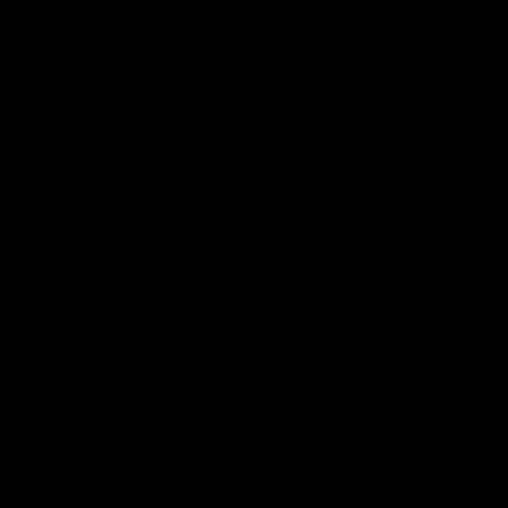
\includegraphics[width=\textwidth]{atelier/breg_cat/cat-0.png}
\subcaption{Iteration $k=0$}
\end{subfigure}\hfill%
\begin{subfigure}{.3\textwidth}%
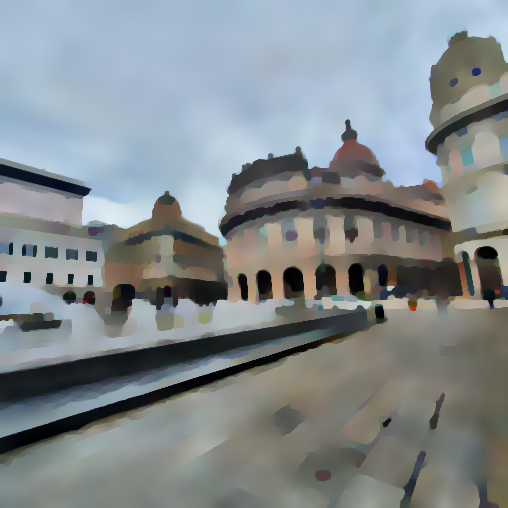
\includegraphics[width=\textwidth]{atelier/breg_cat/cat-10.png}
\subcaption{Iteration $k=10$}
\end{subfigure}\hfill%
\begin{subfigure}{.3\textwidth}%
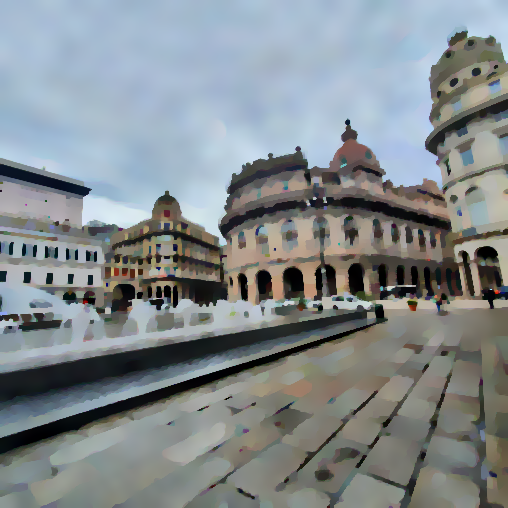
\includegraphics[width=\textwidth]{atelier/breg_cat/cat-20.png}
\subcaption{Iteration $k=20$}%
\end{subfigure}
\end{minipage}\\%

\begin{minipage}{\textwidth}%
\begin{subfigure}{.3\textwidth}%
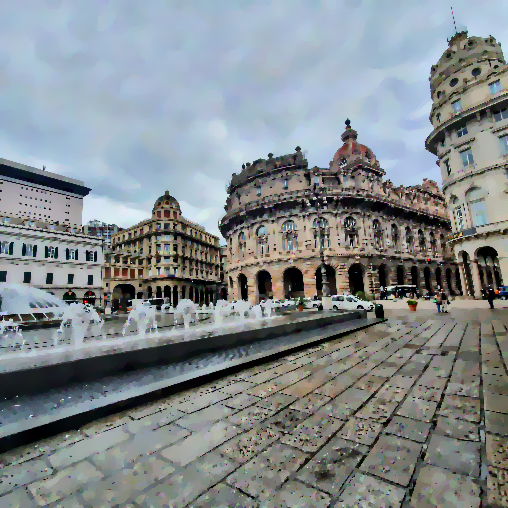
\includegraphics[width=\textwidth]{atelier/breg_cat/cat-50.png}%
\subcaption{Iteration $k=50$}%
\end{subfigure}\hfill%
\begin{subfigure}{.3\textwidth}%
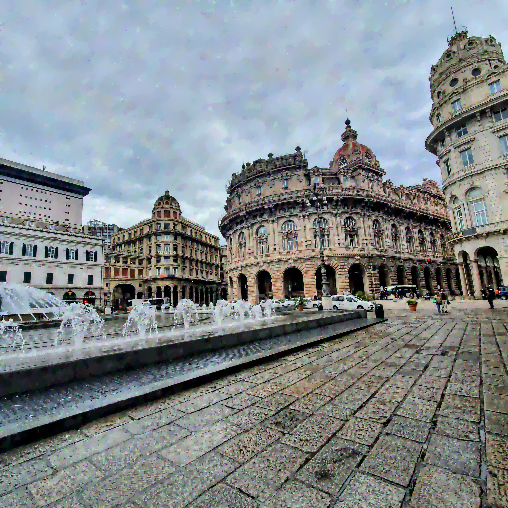
\includegraphics[width=\textwidth]{atelier/breg_cat/cat-95.png}%
\subcaption{Iteration $k=100$}%
\end{subfigure}\hfill%
\begin{subfigure}{.3\textwidth}%
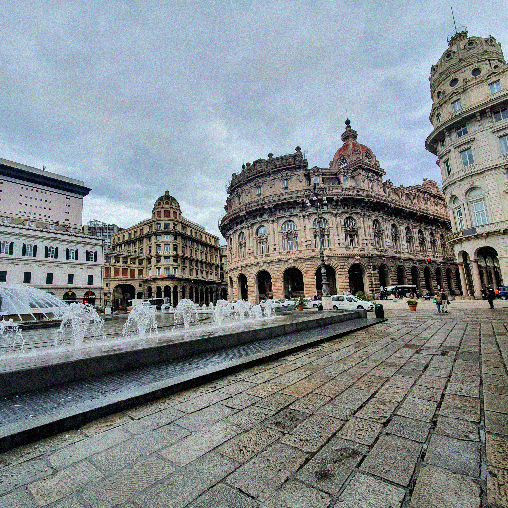
\includegraphics[width=\textwidth]{atelier/breg_cat/data.png}
\subcaption{Iteration $k=500$}
\end{subfigure}%
\end{minipage}%
%
\caption{Bregman iterations for image denoising in \cref{ex:BregCat}}\label{fig:BregCat}
\end{figure}%
%
%
\noindent
If $J=\frac{1}{2}\norm{\cdot}_2^2$ as in \cref{ex:BregNorm} then this amounts to the step
%
\begin{align*}
\param^{(k+1)} &= \argmin_{\param\in\Param} \frac{1}{2}\norm{\param - \param^{(k)}}^2_2 + \tau^{}\empLoss(\param),
\end{align*}
%
where the optimality conditions then yield
%
\begin{align*}
\param^{(k+1)} - \param^{(k)} + \tau \nabla \empLoss(\param^{(k+1)}) = 0
\Leftrightarrow \param^{(k+1)}= \param^{(k)} - \tau \nabla \empLoss(\param^{(k+1)})
\end{align*}
%
which is a standard implicit Euler iteration. The time continuous flow for $\tau\to 0$ is known as the \emph{inverse scale space} flow \cite{burger2006nonlinear,burger2007inverse},
%
\begin{align*}
\begin{cases}
    \dot{\sg}_t = - \nabla\empLoss(\param_t), \\
    \sg_t \in \partial \func(\param_t),
\end{cases}
\end{align*}
%
where again for $J=\frac{1}{2}\norm{\cdot}_2^2$ we obtain that $\partial J(\param_t) = \param_t$ and therefore obtain the standard gradient flow. Hence we see, that the inverse scale space flow is a generalization of the standard gradient flow. 
%
%
%
\subsection{Linearized Bregman Iterations and Mirror Descent}
%
The minimization step in \cref{eq:bregman_iteration} is infeasible for large scale applications, especially in our setting of neural networks. Therefore, we employ the idea introduced in \cite{yin2008bregman, cai2009convergence}. Here, we first linearize the loss function around the previous iterate,
%
\begin{align*}
\empLoss(\param) \approx \empLoss(\param^{(k)}) + 
\left\langle \nabla\empLoss(\param^{(k)}), \param - \param^{(k)}
\right\rangle.
\end{align*} 
%
The next step is to replace $\func$ with the strongly convex elastic net regularization%
\begin{align}\label{eq:elastic_net}
\func_\delta:= \func + \frac{1}{2\delta}\norm{\cdot}^2_2.
\end{align}
%
The minimization step then transforms to
%
\begin{align}\label{eq:LinBregDer}
\argmin_{\param\in\Param} &D^{\sg^{(k)}}_{\func_\delta} \left(\param,\param^{(k)}\right) + \tau^{}\left\langle \nabla\empLoss(\param^{(k)}), \param
\right\rangle\\&= 
\argmin_{\param\in\Param}
J(\param) + \frac{1}{2\delta} \norm{\param}^{2}_2 - 
\langle \sg^{k}, \param\rangle +
\tau^{}\left\langle \nabla\empLoss(\param^{(k)}), \param
\right\rangle\nonumber\\
&=
\argmin_{\param\in\Param}
J(\param) + \frac{1}{2\delta} \norm{\param - \delta(\sg^{(k)} -\tau \nabla\empLoss(\param^{(k)})}^2_2 - \underbrace{\norm{\sg^{(k)} -\tau \nabla\empLoss(\param^{(k)})}^2_2}_{\text{constant in } \param}\nonumber\\
&=
\prox{\delta \func}\left(\delta\left(\sg^{(k)} -\tau \nabla\empLoss(\param^{(k)}\right)\right).\nonumber%
\end{align}
%
Note that here $\sg^{(k)}$ is a subgradient of $J_\delta$ at $\param$ therefore we derive the subgradient update rule
%
\begin{align*}
\sg^{(k+1)} := \sg^{(k)} - \tau \empLoss(\param^{(k)}).
\end{align*}
%
This finally yields the linearized Bregman iterations
%
\begin{subequations}\label{eq:lin_bregman_iteration}
\begin{align}
\sg^{(k+1)} &= \sg^{(k)} - \tau \nabla\empLoss(\param^{(k)}),\\
\param^{(k+1)} &= \prox{\delta J}(\delta \sg^{(k+1)}).
\end{align}
\end{subequations}
%
%
The last line is equivalent to $\sg^{(k+1)}\in\partial J_\delta(\param^{(k+1)})$ for which we obtain the continuous linearized flow
%
\begin{align*}
\dot{\sg}_t &= -\nabla \empLoss(\param_t),\\
\sg_t &\in \partial J_\delta(\param_t),
\end{align*}
%
see \cite{burger2006nonlinear,burger2007inverse}.
%
%
\paragraph{Connections To Mirror Descent}
As already noticed by \cite{villa2023implicit} linearized Bregman iteration are equivalent to mirror descent in some situations. We show the equivalence in the following, where we employ similar arguments as in \cite{beck2003mirror}.
%
One assumes to be given a differentiable and strongly convex function $h:\Param\to\R$, i.e.,
%
\begin{align*}
h(\overline\param) - h(\param) - \langle\nabla h(\param), \overline\param - \param \rangle \geq  
\frac{1}{2} \norm{\overline\param - \param}^2_2
\end{align*}
%
for all $\param,\overline\param\in\Param$. The mirror descent update then reads (\cite{nemirovskij1983problem, beck2003mirror})
%
\begin{align}\label{eq:mirror}
\theta^{(k+1)} = \nabla h^\ast\left(\nabla h\left(\theta^{(k)}\right) - \tau \empLoss(\param^{(k)})\right)
\end{align}
%
where $h^\ast$ denotes the Fenchel conjugate
%
\begin{align*}
h^\ast(\sg) = \sup_{\param} \langle \sg, \param\rangle - h(\param)
\end{align*}
%
with the gradient (see \cite{boyd2004convex})
%
\begin{align*}
\nabla h^\ast(\sg) = \argmax_{\param} \left\{ \langle\sg, \param\rangle - h(\param)\rangle\right\}.
\end{align*}
%
Therefore, we see that \cref{eq:mirror} can be written as
%
\begin{align*}
\param^{(k+1)} &= \argmax_\param
\left\{\left\langle\nabla h\left(\theta^{(k)}\right) - \tau \empLoss(\param^{(k)}), \param \right\rangle - h(\param)\right\}\\
&=
\argmax_\param \left\{-D_h(\param, \param^{(k)})-\tau\left\langle \empLoss(\param^{(k)}), \param \right\rangle\right\}\\
&=
\argmin_\param \left\{D_h(\param, \param^{(k)})+\tau\left\langle \empLoss(\param^{(k)}), \param \right\rangle\right\}
\end{align*}
%
which was our starting point to derive linearized Bregman iterations for $h=\func_{\delta}$ in \cref{eq:LinBregDer}. In fact, we can always find a convex functional $\func:\Theta\to\R$ such that $h = J + \frac{1}{2}\norm{\cdot}_2^2$ for which we see, that \cref{eq:lin_bregman_iteration} is a more general formulation of \cref{eq:mirror}.
%
%
\subsection{Stochastic and Momentum Variants}\label{sec:Bregmom}
%
%
We want to employ linearized Bregman iterations to train a neural network. As mentioned in \cref{sec:SGD} we therefore do not compute the full gradient of $\empLoss$ but rather a minibatched variant. This yields stochastic Bregman Iterations
%

\begin{align}\label{eq:stochlinbreg}
\begin{split}
\text{draw }&\omega^{(k)}\text{ from }\Omega\text{ using the law of }\P,\\
g^{(k)} &:= {g(\param^{(k)};\omega^{(k)})},\\
v^{(k+1)} &:= v^{(k)} - \tau^{(k)} g^{(k)},\\
\param^{(k+1)} &:= \prox{\delta J}(\delta v^{(k+1)}),
\end{split}
\end{align}
%
which we also abbreviate as the \emph{LinBreg} algorithm in the following.
%
The basic update scheme is given as the linearized Bregman iterations from\cite{osher2005iterative}, however the presence of a stochastic gradient estimator significantly complicates the convergence analysis, as observed in \cref{sec:ConvAna}. However, this algorithm can now be efficiently employed to train a neural network. For the analogous stochastic mirror descent algorithm we refer to \cite{nemirovski2009robust}.
%
\paragraph{Momentum Variant} Typically, the learning process of a neural network can be improved by introducing a momentum term (see e.g. \cite{nesterov1983method, qian1999momentum}) in the optimizer. In our case this can be achieved, by replacing the gradient update on the subgradient variable. In \cite{bungert2022bregman} we first consider the inertia version of the gradient flow as
%
\begin{align*}
\begin{cases}
    \gamma \ddot{v}_t + \dot{v}_t = -\nabla\empLoss(\param_t), \\
    v_t \in \partial \func_\delta(\param_t).
\end{cases}
\end{align*}
%
for which the discretization then reads
%
\begin{align}\label{eq:momBreg}
\begin{split}
m^{(k+1)} &= \beta^{(k)} m^{(k)} + (1-\beta^{(k)})\tau^{(k)} g^{(k)},\\
v^{(k+1)} &= v^{(k)} - m^{(k+1)},\\
\param^{(k+1)} &= \prox{\delta\func}(\delta v^{(k+1)}).
\end{split}
\end{align}
%
%
\paragraph{Adamized Bregman Iteration} We shortly remark that one can replace the momentum update in \cref{eq:momBreg} with a Adam update \cite{kingma2014adam}. This then yields an Adamized version of linearized Bregman iterations as employed in \cite{bungert2022bregman}.


\subsection{Convergence of Stochastic Bregman Iterations}\label{sec:ConvAna}
%
%
While various previous works prove convergence of linearized Bregman iterations (see e.g. \cite{osher2005iterative, cai2009convergence}), the stochastic setting requires special treatment. In \cite{bungert2022bregman} the first guarantees for the algorithm in \cref{eq:stochlinbreg} were proven. Other work on convergence of stochastic Bregman iterations, or mirror descent \cite{dragomir2021fast, hanzely2021fastest, zhang2018convergence, d2021stochastic, aubin2022mirror} requires a differentiable functional $\func$. However, since our main motivation is to a functional in the flavor of the $\ell^1$ norm this is not applicable. Therefore, we present the novel convergence analysis of \cite{bungert2022bregman}.
%
%
\paragraph{Assumptions on the Gradient Estimator}
%
In order to obtain convergence guarantees, we need to assume mainly two properties on the gradient estimator $g(\cdot,\cdot)$. First we assume unbiasedness, which means
%
\begin{align*}
\Exp{g(\param;\omega)} = \nabla\empLoss(\param)\text{ for all }\param\in\Param.
\end{align*}
%
The second assumption we need in the following is referred to as \emph{bounded variance} of the estimator.
%
\begin{assumption}{Bounded variance}{ass:variance}
There exists a constant $\sigma>0$ such that for any $\param\in\Param$ it holds
\begin{align}
    \E\left[\norm{g(\param;\omega)-\nabla\empLoss(\param)}^2\right] \leq \sigma^2.
\end{align}
\end{assumption}
%
%
\begin{remark}{}{}
We want to remark, that this property is weaker than the bounded gradient assumption
%
\begin{align*}
\E\left[\norm{g(\param;\omega)}^2\right] \leq C
\end{align*}
%
for some constant $C>0$. In fact this condition can not be enforced together with a strong convexity assumption---which we employ in \cref{thm:??}---as shown in \cite{pmlr-v80-nguyen18c}.
\end{remark}
\paragraph{Assumptions on the Regularizer and on the Loss Function}
%
The assumptions on the regularization functional $\func$ are mild and merely ensure the well-definedness of the proximal mapping,
%
%
\begin{assumption}{Regularizer}{ass:regularizer}
We assume that $\func:\Param\to(-\infty,\infty]$ is a convex, proper, and lower semicontinuous functional on the Hilbert space $\Param$.
\end{assumption}
%
%
Our assumptions on the loss function $\empLoss$ are more restrictive. We require it to be bounded from below and differentiable, which are both standard assumptions. Additionally, we require Lipschitz continuity of the gradient, which also commonly employed in optimization literature.
%
\begin{assumption}{Loss function}{ass:loss}
We assume the following conditions on the loss function:
\begin{itemize}
    \item The loss function $\empLoss$ is bounded from below and without loss of generality we assume $\empLoss\geq 0$.
    \item The function $\empLoss$ is continuously differentiable.
    \item The gradient of the loss function $\param\mapsto\nabla\empLoss(\param)$ is $L$-Lipschitz for $L\in(0,\infty)$:
    \begin{align}\label{ineq:gradLip}
        \norm{\nabla\empLoss(\tilde\param)-\nabla\empLoss(\param)}\leq L \norm{\tilde\param-\param},\quad \forall \param,\tilde\param\in\Param.
    \end{align}
\end{itemize}
\end{assumption}
%
%
If the loss function $\empLoss$ fulfills the previous assumptions we are able to prove loss decay of the iterates in \cref{thm:decreasingloss}. However, in order to show convergence of the iterates we additionally need a convexity assumption. For a differentiable functional $J$, the authors in \cite{dragomir2021fast} assumed
%
\begin{align*}
\nu\ D_J(\pparam,\param) \leq D_\empLoss(\pparam,\param)
\end{align*}
%
which for twice differentiable $\func,\empLoss$ transfers to
%
\begin{align*}
\nu\ \nabla^2 \func \lesssim \nabla^2 \empLoss,\qquad\forall\pparam,\param\in\Param.
\end{align*}
%
Plugging in the definition of the Bregman dist $D_\empLoss$ we obtain
%
\begin{align*}
\nu\ D_J(\pparam,\param) \leq \empLoss(\pparam) - \empLoss(\param) - 
\langle \nabla\empLoss(\param), \pparam-\param\rangle.
\end{align*}
%
In this form one observes that this is in fact a convexity assumption on $\empLoss$ in a $\func$ dependent distance, as employed in \cite{bungert2022bregman}.
%
%
\begin{assumption}{Strong convexity}{ass:muconvex} 
For a proper convex function $H:\Param\to\R$ and $\nu\in(0,\infty)$, we say that the loss function $\param\mapsto\empLoss(\param)$ is $\nu$-strongly convex w.r.t. $H$, if
\begin{align}
\empLoss(\pparam) \geq \empLoss(\param) + \langle\nabla\empLoss(\param), \pparam - \param\rangle + \nu D_\func^\sg(\pparam,\param),\quad\forall\param,\pparam\in\Param, \sg\in\partial H(\param).
\end{align}
\end{assumption}
%
%
\begin{remark}{}{}
We have two relevant cases for the choice of $H$. For $H=\frac{1}{2}\norm{\cdot}^2$ \cref{ass:muconvex} reduces to standard strong $\nu$-convexity. The other relevant case, is $H=J_\delta$, i.e. we consider convexity w.r.t. to the functional $J_\delta$.
\end{remark}
%
%
\begin{remark}{}{}
In the setting of training a neural network, where we employ the empirical loss \cref{eq:empLoss}, this convexity assumption usually fails. While it is possible to enforce this conditions only locally around the minimum, this does not significantly improve the applicability. For future work, it would be desirable to enforce a  Kurdyka--\L ojasiewicz inequality, as in \cite{benning2018choose} for the deterministic case. 
\end{remark}

\paragraph{Loss Decay}
The first convergence result considers the loss decay of the iterates. Here, we do not assume convexity of the loss function. Under this assumptions \cite{benning2018choose, benning2018modern} were able to show the inequality
%
\begin{align*}
\begin{split}
\E\left[\empLoss(\param^{(k+1)})\right] + \frac{1}{\tau^{(k)}}\E\left[ D^\mathrm{sym}_\func(\param^{(k+1)},\param^{(k)})\right] + \frac{C}{2\delta\tau^{(k)}}\E\left[\norm{\param^{(k+1)}-\param^{(k)}}^2\right] \\
\leq \E\left[\empLoss(\param^{(k)})\right].
\end{split}
\end{align*}
%
%
In our setting, employing a stochastic gradient estimator, we are able to prove a similar estimate. Here, we obtain an additional term scaled $\sigma$ which controls the expected squared difference between the gradient estimator and the actual gradient. It should however be noted, that the proof is not only a trivial extension.
%
%
\begin{theorem}{\cite[Th. 2]{bungert2022bregman}: Loss decay}{thm:decreasingloss}
Assume that \cref{ass:loss,ass:variance,ass:regularizer} hold true, let $\delta>0$, and let the step sizes satisfy $\tau^{(k)} \leq \frac{2}{\delta L}$.
Then there exist constants $c,C>0$ such that for every $k\in\N$ the iterates of \labelcref{eq:stochlinbreg} satisfy 
\begin{align}\label{ineq:loss_decay}
    \begin{split}
    \E\left[\empLoss(\param^{(k+1)})\right] + \frac{1}{\tau^{(k)}}\E\left[ D^\mathrm{sym}_\func(\param^{(k+1)},\param^{(k)})\right] + \frac{C}{2\delta\tau^{(k)}}\E\left[\norm{\param^{(k+1)}-\param^{(k)}}^2\right] \\
    \leq \E\left[\empLoss(\param^{(k)})\right] + \tau^{(k)}\delta\frac{\sigma^2}{2c},
    \end{split}
\end{align}
\end{theorem}

\paragraph{Convergence of the Iterates}
Here, we have two cases respectively proving convergence w.r.t. the $L^2$ distance and the Bregman distance of $\func_\delta$. The first assumes strong convexity with $H=\frac{1}{2}\norm{\cdot}^2$ in \cref{ass:muconvex}.
%
%
\begin{theorem}{\cite[Th. 6]{bungert2022bregman}: Convergence in norm}{thm:cvgc_norm}
Assume that \cref{ass:loss,ass:variance,ass:regularizer} and \cref{ass:muconvex} for $H=\frac{1}{2}\norm{\cdot}^2$ hold true and let $\delta>0$.
Furthermore, assume that the step sizes $\tau^{(k)}$ are such that for all $k\in\N$:
\begin{align*}
    {\tau^{(k)}\leq \frac{\mu}{2\delta L^2}},\qquad
    \tau^{(k+1)} \leq \tau^{(k)}, \qquad
    \sum_{k=0}^\infty (\tau^{(k)})^2 < \infty, \qquad
    \sum_{k=0}^\infty \tau^{(k)} = \infty.
\end{align*}
The function $\mathcal{L}$ has a unique minimizer $\param^*$ and if $J(\param^*)<\infty$ the stochastic linearized Bregman iterations \labelcref{eq:stochlinbreg} satisfy the following:
\begin{itemize}
    \item Letting $d_k:=\E\left[D_{\func_\delta}^{v^{(k)}}(\param^*,\param^{(k)})\right]$ it holds
    \begin{align}\label{ineq:decay_bregman_distance}
        d_{k+1} - d_k + \frac{\mu}{4}\tau^{(k)}\E\left[\norm{\param^*-\param^{(k+1)}}^2\right]
        \leq  \frac{\sigma}{2}\left((\tau^{(k)})^2 +\Exp{\norm{\param^{(k)} - \param^{(k+1)}}^2}\right).
    \end{align}
    \item The iterates possess a subsequence converging in the $L^2$-sense of random variables: 
    \begin{align}
        \lim_{j\to\infty}\E\left[\norm{\param^*-\param^{(k_j)}}^2\right] = 0.
    \end{align}
\end{itemize}
{Here, $\func_\delta$ is defined as in \labelcref{eq:elastic_net}.}
\end{theorem}
%
%
For the second result we assume convexity w.r.t. the Bregman distance, i.e. we choose $H=\func_{\delta}$ in \cref{ass:muconvex}. This induces a relation between the Bregman distance of $\func$ and the loss function $\empLoss$, which has been similarly employed in \cite{dragomir2021fast}.
%
%
\begin{theorem}{\cite[Th. 11]{bungert2022bregman}: Convergence in the Bregman distance}{thm:cvgc_breg_dist}
Assume that \cref{ass:loss,ass:variance,ass:regularizer} and \cref{ass:muconvex} for $H=J_\delta$ hold true and let $\delta>0$.
The function $\mathcal{L}$ has a unique {minimizer} $\param^*$ and if $\func(\param^*)<\infty$ the stochastic linearized Bregman iterations \labelcref{eq:stochlinbreg} satisfy the following:
\begin{itemize}
    \item {Letting $d_k :=\E\left[D_{J_\delta}^{v^{(k)}}(\param^*,\param^{(k)})\right]$ it holds
    \begin{align}\label{eq:estimate_expects}
        % d_{k+1} \leq \left(1 - \tau^{(k)}\nu\right)d_k + (\tau^{(k)})^2\delta B.
        d_{k+1} \leq \left[1 - \tau^{(k)}\nu\left(1-\tau^{(k)}\frac{2\delta^2 L^2}{\nu}\right)\right]d_k + \delta(\tau^{(k)})^2\sigma^2.
    \end{align}}
    \item For any $\eps>0$ there exists $\tau>0$ such that if $\tau^{(k)}=\tau$ for all $k\in\N$ then
    \begin{align}
        \limsup_{k\to\infty} d_k \leq \eps.
    \end{align}
    \item If $\tau^{(k)}$ is such that
    \begin{align}\label{eq:cond_step_size}
        \lim_{k\to\infty} \tau^{(k)} = 0 \quad \text{and}\quad \sum_{k=0}^\infty \tau^{(k)} = \infty
    \end{align}
    then it holds
    \begin{align}
        \lim_{k\to\infty} d_k = 0.
    \end{align}
\end{itemize}
{Here, $\func_\delta$ is defined as in \labelcref{eq:elastic_net}.}
\end{theorem}
%
%
%
\subsection{Numerical Results and Practical Considerations}\label{sec:Bregnum}
%
%
\begin{wrapfigure}{r}{.4\textwidth}
\begin{center}

\includegraphics[width=.4\textwidth]{atelier/Breg_dist/BregQR.png}
\end{center}
The code for all the experiments is available at \href{https://github.com/TimRoith/BregmanLearning}{github.com/TimRoith/}\\
\href{https://github.com/TimRoith/BregmanLearning}{BregmanLearning}.
\end{wrapfigure}
Before briefly reviewing the numerical results in \cite[Sec. 4]{bungert2022bregman}, we remark on some practical considerations. In particular we comment on the parameter initialization strategy. All the experiments were implemented in \texttt{Python} \cite{van1995python} employing---among others---the \texttt{PyTorch} \cite{paszke2019pytorch}.
%
\paragraph{Parameter Initialization} As already noticed in \cite{bengio10} parameter initialization has a significant impact on the training of the neural network. Here, in contrast to standard Bregman methods, we are not able to initialize the parameters of the neural network as $\param=0$. This is due to that fact, that a zero initialization induces symmetries in the network weights, for which one cannot utilize the full expressivity of the architecture \cite[Ch. 6]{Goodfellow16}. Therefore, we rather employ the approach from \cite{liu2021,dettmers2019sparse,martens2010deep} of sparsifying weight matrices $\tilde W^l\in\R^{n_{l+1}\times n_l}$ up to a certain level, by a pointwise multiplication with a binary mask $M^l\in{0,1}^{n_{l+1}\times n_l}$
%
\begin{align*}
W^l := \tilde W^{l} \odot M^l.
\end{align*}
%
%
Each entry in $M^l$ is i.i.d. sampled from a Bernoulli distribution
%
\begin{align*}
M^l_{i,j}\sim \mathcal{B}(r).
\end{align*}
%
where the parameter $r$ determines the sparsity,
%
\begin{align*}
\mathrm{N}(W^l):=\frac{\norm{W^l}_0}{n_l \cdot n_{l-1}}=
1 - \mathrm{S}(W^l)
\end{align*}
%
with $\mathrm{N}$ denoting the percentage of used parameters and $\mathrm{S}$ the sparsity.
%
%
In \cite{bengio10} the authors advise to especially control to the variance of the parameter initialization distribution, for which in \cite{bungert2022bregman} we derive
%
\begin{align}\label{eq:initcond2}
\Var{\tilde W^l} = \frac{1}{r}~\Var{\tilde W^l \odot M^l}
\end{align}
%
and therefore scale the weights with the sparsity parameter $r$ at initialization.
%
%
\paragraph{Choice of Regularizers}
%
In all our experiments we choose a $L^1$ type sparsity promoting regularization function functional $\func$. We do not employ any coupling between weight matrices of different layers, and therefore for $\param=((W^1,b^1),\ldots, (W^L,b^L))$ we have
%
\begin{align*}
\func(\param) = \sum_{l=1}^L \func^l(W^l)
\end{align*}
%
%
where $\func^l$ is choosen according to the layer type. In the easiest case of a fully connected layer, we can choose
%
\begin{align*}
\func^l(W^l) := \norm{W^l}_1.
\end{align*}
%
In the case of a convolutional layer we have that $W^l$ is determined by convolutional kernels $K_{i,j}\in\R^{k\times k}$, see \cref{sec:convlayer}. Here, we typically employ a group sparsity term in the form
%
\begin{align*}
\func^l(W^l) = \norm{W^l}_{2,1} = \sum_{i,j} \norm{K_{i,j}}_2.
\end{align*}
%
The outer sum acts as a $L^1$ regularizer on the instances $\norm{K_{i,j}}$. Sparsity in this sense, then amounts to having indices $(i,j)$ for which $\norm{K_{i,j}}_2=0 \Leftrightarrow K_{i,j}=0$, i.e., we prune away whole convolutional filters. This effect is displayed in \cite[Fig. 1]{bungert2022bregman}.
%s
We can also employ group sparsity on fully connected layers, by considering row sparsity of $W^l\in\R^{n_{l+1}, n_l}$s
%
\begin{align*}
\func^l(W^l) = \sum_{i=1}^{n_{l+1}} \norm{W_{i,:}}_2 = \sum_{i=1}^{n_{l+1}} \sqrt{\sum_{js=1}^{n_{l}} W_{i,j}^2}.
\end{align*}
%
%
%
In this setting we have a $L^1$ penalty on the row norms $\norm{W_{i,:}}_2$ which therefore enforces whole rows to be zero. This is relevant, if we employ a layer architecture with $\Psi^l(0)=0$, e.g., using no bias vectors and the ReLU activation function. In this setting, if the $i$th row of $W^l$ is zero this effectively means, that the $i$th neuron in layer $l+1$ is inactive. This observation allows the neural architecture search in one of the following paragraphs.
\paragraph{Comments on the Numerical Results} We briefly remark on the numerical results as displayed in \cite[Sec. 4]{bungert2022bregman}. In the experiments we employed feed-forward networks with simple linear, convolutional and residual layers and tested on the three datasets \cite{krizhevsky2009learning, Han17, leCun10}.

The basic comparison between the  algorithms SGD, ProxGD and LinBreg shows the qualitative behaviour of each iterations. Infantilizing sparse does not have any effect on SGD, since it does not preserve the sparsity in any way. ProxGD rather starts with many active parameters and reduces the this number during the iteration. Only the discretization of the inverse scale space flow---via Bregman iterations---shows the desired behaviour of gradually adding active parameters. Furthermore, in \cite[Fig. 2]{bungert2022bregman} we can see, that the choice of $\lambda$ in the regularizer $\func = \lambda\, \norm{\cdot}_1$ changes the results significantly. In the light of \cref{eq:Bregexact} this is not expected for the standard Bregman iterations with a convex loss. It is therefore interesting to see, that in our non-convex and stochastic situation this effect changes.

The momentum variants, as discussed in \cref{sec:Bregmom} yield the desired effect of enhancing the validation accuracy, and respectively converging faster. However in each  of the experiments, one can also observe that adding a momentum term has the effect that more parameters are added faster. On the one hand this could mean that the network actually requires more parameters to have a higher accuracy, for which a momentum variant is more likely to increase the number of needed parameters. However, the quantitative evaluation on the CIFAR10 dataset \cite{krizhevsky2009learning} shows, that especially the Adamized version tends to increase the number of used parameters rather aggressively, while only slightly increasing the performance of the net. The performance here is very similar to the one of proximal gradient descent. However, the training of a residual network seems to be slightly better with a standard Lasso implementation. Here, one neglects the non-differentiability of the $L^1$ norm and computes a derivate via automatic differentiation \cite{rall1981automatic, maclaurin2015autograd} (we employed the \texttt{autograd} library of the \texttt{PyTorch} package \cite{paszke2019pytorch}). In order to obtain true zeros in the weight matrix one then has to employ a thresholding operation after the training. In some sense this method is not a proper sparse training approach, but rather a regularization method with an added pruning step at the end.

\paragraph{Comments on Efficiency} One of the major advantages of the Bregman approach, is that the network is sparse already during the training time. As with all sparse-to-sparse training approaches this yields a very small number of active parameters over all training step. This sparsity can be easily exploited in each forward pass. However, it is not directly possible to achieve performance gains during the backward pass of the network, since in general
%
\begin{align*}
W^l_{ij} = 0 \nRightarrow \partial_{W^l_{ij}} \empLoss(\theta) = 0.
\end{align*}
%
In \cite{bungert2022bregman, bungert2021neural} there are no evaluation on the training time and memory consumption of the Bregman algorithm. Since the complexity does not increase in comparison to the standard SGD, one hopes to obtain a faster training time here. This is an interesting open question for future work. It should however be remarked that the computational complexity of the LinBreg algorithm does not increase significantly, compared to SGD, since the evaluation of the proximal operator is very efficient for $L^1$ type functionals.

\paragraph{Neural Architecture Search} An interesting aspect hinted in \cite{bungert2022bregman} is optimizing the architecture of a neural network via sparsity. In the example provided in \cite[Fig. 4]{bungert2022bregman} one defines a super-architecture as multi-layer perceptron with an equal number of neurons in each layer. Training this task with the LinBreg algorithm reveals the well-known autoencoder structure \cite{hinton1993autoencoders}. This idea was developed further in \cite{bungert2021neural}, where also skip connection of a residual architecture were learned. Here, the super-architecture was given by a dense net \cite{huang2017densely}, where a each skip connection was scaled by a parameter, which was penalized with a sparsity term. The driving question here, if it is possible also learn an architecture similar to the U-Net as proposed in \cite{ronneberger2015u}.
%
%
%
%
\clearpage%
%
\section{Resolution Stability via FNOs: \cite{kabri2023resolution}}\label{sec:FNO}
%
\setlength\intextsep{0pt}
\begin{wrapfigure}{r}{.5\textwidth}
\centering
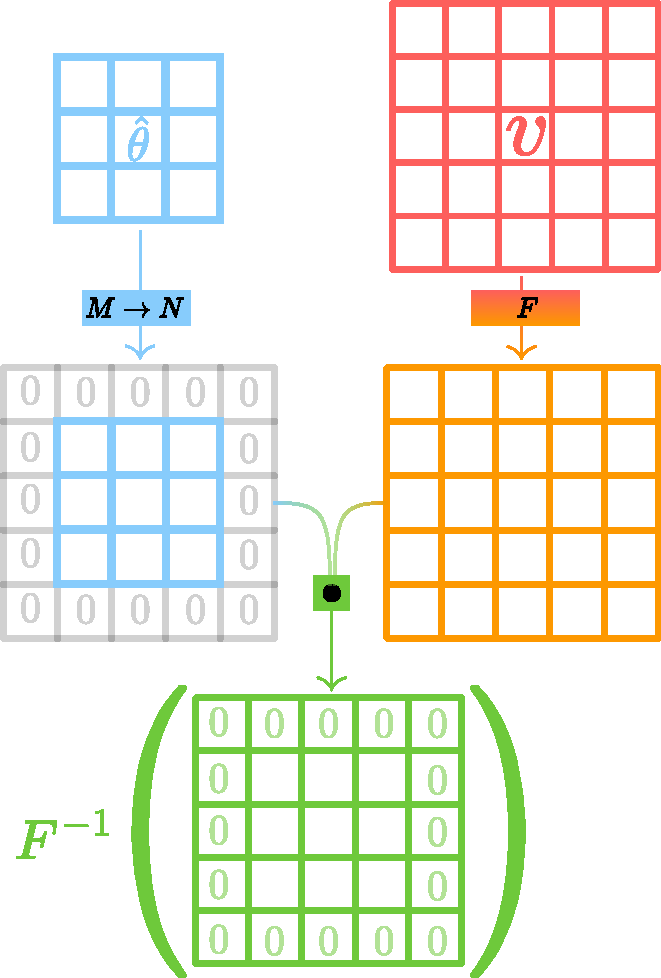
\includegraphics[width=.4\textwidth]{atelier/FNO/trigo.pdf}
\end{wrapfigure}
%
We frequently employ the set $\Inp=[0,1]^{K\times N\times M}$ to represent images. However, from a modeling point of view it is more natural to assume that images are functions $\img:\domain\to[0,1]^K$ where $\domain\subset\R^2$ is some domain. In this sense, the space $\Inp$ only constitutes a discretization of the space of all functions from $\domain$ to $[0,1]^K$. The number of pixels, i.e. $N\cdot M$, relates to the \emph{resolution} of the image, where a higher number of pixels yields a higher resolution. In this sense the resolution is merely an artifact of the restriction to finite dimensions in computer vision and not relevant for the classification. Therefore, one wants to obtain a resolution-independent classifier, which we study in the following.
%
\paragraph{Images, Resolution and Scale}
%
%
For the continuum domain we consider the $d$-dimensional torus $\domain = \mathbb{R}^d / \mathbb{Z}^d$. An image is a function 
%
\begin{align*}
\img:\domain\to[0,1]^K
\end{align*}
%
where $K\in\N$ denotes the number of color channels, see \cite{gonzales1987digital}. In order to represent images on a computer we discretize the domain $\domain$, via a regular grid $\domain_N = \{x_0,\ldots,x_N\}$ indexed by the set
%
\begin{align*}
\mathcal{J}_N := \{0,\ldots, N-1\}^d
\end{align*}
%
with grid points $x_j = j/(N-1)$, see e.g. \cite{kabri2022FNO, kovachki2021universal}. For simplicity we assume an equal number of discretization points in each dimension. Therefore, $N^d$ is the resolution of an image discretized w.r.t. $\mathcal{J}_N$. 

It is important to notice the differences to the concept of \emph{scale}. A change in scale would be a change in the original image domain, for example by zooming in on a certain area. For our image classification examples, we usually assume that the image $\img$ contain a certain entity to be classified. The scale roughly describes how \enquote{big} the entity is, or what percentage of the image it fills. We assume that the scale is fixed. Therefore, changing $N$ directly influences the resolution of discretization.

\paragraph{How do Neural Networks react to Resolution Changes?} In many machine learning application one assumes a fixed input size and therefore a fixed resolution, assuming the same scale throughout the data. Formally, networks are defined as mappings $\net_\param:\R^{K\times N\times N}\to\Delta^C$, i.e. they only accept inputs for the fixed resolution $N$. In order to understand how this constraint can be weakened, we need to consider the concrete structure of our networks, which was similarly done in \cite{kovachki2021universal, kabri2022FNO}. The architectures we consider are feed-forward networks of the form
%
\begin{align*}
\net_\param = \Phi^{\text{class}} \circ \mathcal{S}\circ \Phi^{\text{feature}}
\end{align*}
%
where 
%
\begin{itemize}
\item $\Phi^{\text{feature}}$ is the so-called feature extractor, which should be applicable independently from the input dimension,
\item $\mathcal{S}$ is a function that maps inputs of any size to a fixed output dimension $\R^s$,
\item $\Phi^{\text{class}}:\R^s\to\Delta^C$ denotes the classification layer.
\end{itemize}
%
%
%
The feature extractor usually consists of convolutional layers. As in \cite[Ch. 2]{kabri2022FNO} we consider the discrete convolution of two discretized images $\img_N, \imgg_N$ defined as 
%
\begin{align*}
(\img_N\ast \imgg_N)(x_j) := \sum_{k\in \mathcal{J}_N} \img_N(x_k)\cdot \imgg_N(x_{j-k})
\end{align*}
%
where for negative indices $j-k$ we set $x_{j-k} := x_{j-k+N}$. This assumes that both $\img_N, \imgg_N$ live on the same discretization $\mathcal{J}_N$. Modeling spatial locality---and therefore a small support of the kernel---one usually chooses $M$ much smaller than the resolution. See e.g. the study in \cite{hubel1962receptive} which explores a similar methodology for the visual cortex of cats. In order to account for this dimension mismatch we consider so-called \emph{spatial zero-padding} for kernels $\param\in\R^{\mathcal{J}_M}$
%
\begin{align*}
\param^{M \rightarrow N}_k = 
\begin{cases}
\param_k & \text{for } k \in \mathcal{J}_N \cap \mathcal{J}_M,\\
0 & \text{for } k \in \mathcal{J}_N \backslash \mathcal{J}_M.
\end{cases}
\end{align*}
%
Using this method, one can define the convolution for inputs $u_N$ of arbitrary input resolution $N$ via
%
\begin{align*}
C(\param)(u_N)= \param^{M \rightarrow N} \ast u_N.
\end{align*}
%
In \cite{kabri2023resolution} we refer to this as the \emph{spatial implementation} of convolution. Up to the behavior on the boundary this is in fact the standard implementation in most libraries, especially in \texttt{PyTorch}. Therefore, a feature extractor consisting of convolutional layers can take inputs of variable resolution. In fact, ignoring possible resolution changes within the extractor---i.e. via pooling or strided convolutions---we have that $\Phi^{\text{feature}}(\img_N)\in \R^{\mathcal{J}}_N$ for any $N\in\N$.

The mapping $\mathcal{S}$ can be realized as an adaptive pooling layer, see \cite{paszke2019pytorch}, which ensures a fixed output size. This methodology yields an \emph{discretization invariant architecture}, see \cite{kabri2022FNO, kovachki2021universal, li2020fourier}, which means that from a technical point of view the network is able to produce outputs for inputs with arbitrary discretization. However, we are actually interested in \emph{discretization invariant functionality} (see \cite{kabri2022FNO, kovachki2021universal, li2020fourier}), which also requires that the output is the same over different resolutions.
%
\paragraph{Input Interpolation}
%
%
The technical possibility to handle different input sizes as described above, usually does not perform well in practice. This is due to the fact that in the standard spatial implementation of convolution the support of the kernel changes with varying input dimension, for which it output differs, see \cref{fig:bulbul}. If a network is trained on a fixed input size, the filters are adapted to this size and therefore only create meaningful responses on this size.

A simple attempt to create a network, where not only the architecture, but also the functionality is discretization independent---at least up to a certain degree---is input interpolation. In this case our architecture is modified to
%
\begin{align*}
\tilde \net_\param = \net_\param \circ I
\end{align*}
%
where $I:\bigcup_{M\in\N} \R^{\mathcal{J}_M} \to \R^{\mathcal{J}_N}$ is an interpolation function, that maps inputs of arbitrary sizes to a fixed out discretization $\mathcal{I}_N$. Typical choices here include nearest neighbor, bilinear or bicubic interpolation, see e.g. \cite{gonzales1987digital}. Especially relevant in our case, is so-called \emph{trigonometric interpolation}, where for $\imgg_M\in\R^{\mathcal{J}}$ we define
%
%
\begin{align*}
I^{\text{trigo}}(\imgg_M) := \imgg_M^{M \xrightarrow{\Delta} N} := F^{-1} \left( (Fv)^{M \rightarrow N}\right).
\end{align*}
%
%
\paragraph{Contribution} In \cite{kabri2023resolution} we study the connection between FNOs and CNNs for classification problems. We identify under which assumption the architectures are equivalent (see \cref{lem:FNOconv}), but also where they are not, see \cref{fig:bulbul}. Here, we are especially interested in the multi-resolution case, we show that one layer of an FNO is equivariant with respect to trigonometric interpolation, \cref{cor:FNOequi}. This is also underlined by numerical experiments, where we compare the FNO implementation to interpolation methods and a naive CNN implementation. Furthermore, we show that training equivalent CNN and FNO layers lead to different results, i.e., while they have the same forward pass, the gradients w.r.t. their parameters might differ, \cref{lem:FNOGrad}. Furthermore, we show continuity and Fréchet-differentiability of abstract neural layers as operators between $L^p$ spaces, see \cref{sec:FNOAna}. Finally we conduct numerical experiments supporting our theoretical findings \cref{sec:FNONum}.
%
%

%
%
\subsection{Fourier Neural Operators}
%
%
We want to obtain neural networks whose output does not depend on the discretization of an image $\img:\domain\to\R^K$. This raises the question whether it is possible to find a formulation that allows us to work in the infinite dimensional setting. In \cite{kovachki2021neural} this issue was addressed in the setting of parametric PDEs for which the authors introduced the concept of \emph{neural operators}. One layer of a neural operator is given as a mapping $\mathcal{G}:  L^p(\domain) \rightarrow L^q(\domain)$
%
\begin{align}\label{eq:layerdef}
\mathcal{G}(u)(x) = \sigma\left(\Psi(u)(x)\right) \qquad \text{for a.e. } x \in \domain,
\end{align}
%
with the affine linear part given by
%
\begin{align}\label{eq:linearpart}
\Psi(u) = W u + \mathcal{K}u + b,
\end{align}
%
where
%
\begin{itemize}
\item $\mathcal{K}: u \mapsto \int_{\domain} \kappa(\cdot, y)\, u(y)\,dy$ is a kernel integral operator with kernel $\kappa: \domain \times \domain \rightarrow \R$,
\item $W \in \R$ models a residual component,
\item and $b: \domain \rightarrow \R$ models a bias.
\end{itemize}
%
%
By a slight abuse of notation, the activation function $\sigma:\R\to\R$ acts as a \Nem operator
%
\begin{align}\label{eq:nemytskii}%
\sigma: v \mapsto \sigma(v(\cdot)),
\end{align}
%
see e.g. \cite{tröltzsch}.

In \cref{sec:FNOAna} we analyze continuity and differentiablility of a layer in this abstract form. However, the most relevant case for us, is when $\mathcal{K}$ is a convolution operator, i.e. $\kappa(x,y)=\kappa(x-y)$ is a translation invariant kernel. In this special case $\mathcal{G}$ is then known as layer of a \emph{Fourier Neural Operator} (FNO) as introduced in \cite{li2020fourier}, by parameterizing the kernel via its Fourier coefficients $\hat{\param}_k\in\C$
%
\begin{align}\label{eq:fnokernel}
\kappa_{\hat{\theta}}(x) = \sum_{k \in \mathcal{I}} \hat{\theta}_k\, b_k(x),
\end{align}
%
where $b_k(x) = \exp{(2\pi i\, kx)}$ denote the Fourier basis functions. In practice we assume that $\kappa_{\hat\param}$ only has a finite amount of non-zero Fourier coefficients, in fact we choose the set $\mathcal{I}_N := \lbrace -\lceil (N-1)/2\rceil, \ldots,0, \ldots\,, \lfloor (N-1)/2 \rfloor\rbrace^d$ as the index set, as done in \cite{li2020fourier}. Employing this set with odd $N\in\N$, we can easily enforce Hermitian symmetry $\hat{\theta}_k = \overline{\hat{\theta}_{-k}}$, which ensures that $\mathcal{K}_{\hat\param}$ outputs real-valued functions. For now we assume an odd number here and deal with the even case later. We note that assuming a finite number $N$ of Fourier coefficients is completely independent from the input discretization, which is the main advantage of FNOs.
%
%
\paragraph{How to Perform Convolutions with FNOs?}
%
%
In \cite{kabri2023resolution} we consider the discrete Fourier transform and its inverse
%
\begin{align*}
\left(Fv\right)_k &= \frac{1}{\lambda} \sum_{j \in \mathcal{J}_N} v_j\, e^{-2\pi i \, \left\langle k, \frac{j}{N}\right\rangle},  k \in \mathcal{I}_N,\\
%
\left(F^{-1}\hat{v}\right)_j &= \frac{\lambda}{|\mathcal{J}_N|}\sum_{k \in \mathcal{I}_N} \hat{v}_k\, e^{2\pi i \, \left\langle k, \frac{j}{N}\right\rangle} j \in \mathcal{J}_N,
\end{align*}
%
with a normalization constant $\lambda \in \{1, \sqrt{|\mathcal{J}_N|}, |\mathcal{J}_N|\}$. We only consider parameters $\hat\param\in \Csym^{\mathcal{I}_N} := F(\R^{\mathcal{J}_N})$ for which can employ the convolution theorem (see e.g. \cite{grafakos}) to define
%
\begin{align}\label{eq:discfno}
K(\hat{\theta})(v) = F^{-1}\left(\hat{\theta} \cdot Fv\right) \qquad \text{for }v \in \R^{\mathcal{J}_N}
\end{align}
%
which is referred to as the FNO- or spectral-implementation of convolution.
%
%
\paragraph{How do FNOs React to Resolution Changes?}
%
We already mentioned that the number of Fourier coefficients of $\hat\param\in\Csym^{\mathcal{I}_M}$ is independent of the input resolution. Nevertheless, the point-wise multiplication in \cref{eq:discfno} is only defined for inputs $\imgg\in\R^{\mathcal{J}_M}$, for which the question arises how FNOs can be adapted to dimension mismatch. Here, we apply a conceptually similar idea, by employing zero-padding. However, the important and major difference is that this zero-padding is performed in the spectral domain. Assuming that $N>M$ is odd and that $\imgg_N\in\R^{\mathcal{J}_N}$ we define
%
%
\begin{align*}
\hat{\theta}^{M \rightarrow N}_k = \begin{cases}
\hat{\theta}_k & \text{for } k \in \mathcal{I}_N \cap \mathcal{I}_M,\\
0 & \text{for } k \in \mathcal{I}_N \backslash \mathcal{I}_M,
\end{cases}
\end{align*}
%
%
and the spectral implementation of convolution as
%
%
\begin{equation*}
   K(\hat{\theta})(\imgg_N) := K(\hat{\theta}^{M \rightarrow N})(\imgg_N).
\end{equation*}
%
%
\paragraph{What Is The Difference Between Standard and FNO Implementation?}
%
%
The difference between the spectral and spatial implementation is best explained with \cite[Fig. 1]{kabri2023resolution}, which we repeat in \cref{fig:bulbul} for convenience.
%
%
\begin{figure}[t]
\begin{minipage}[t]{\textwidth}
%\fbox{%
\begin{minipage}{\textwidth}
\begin{minipage}{0.01\textwidth}%
\rotatebox{90}{%
	\scriptsize%
	higher resolution \phantom{------------} 
	original \phantom{-------------} 
	lower resolution\phantom{--}}
\end{minipage}%
\hfill%
\begin{minipage}{0.95\textwidth}
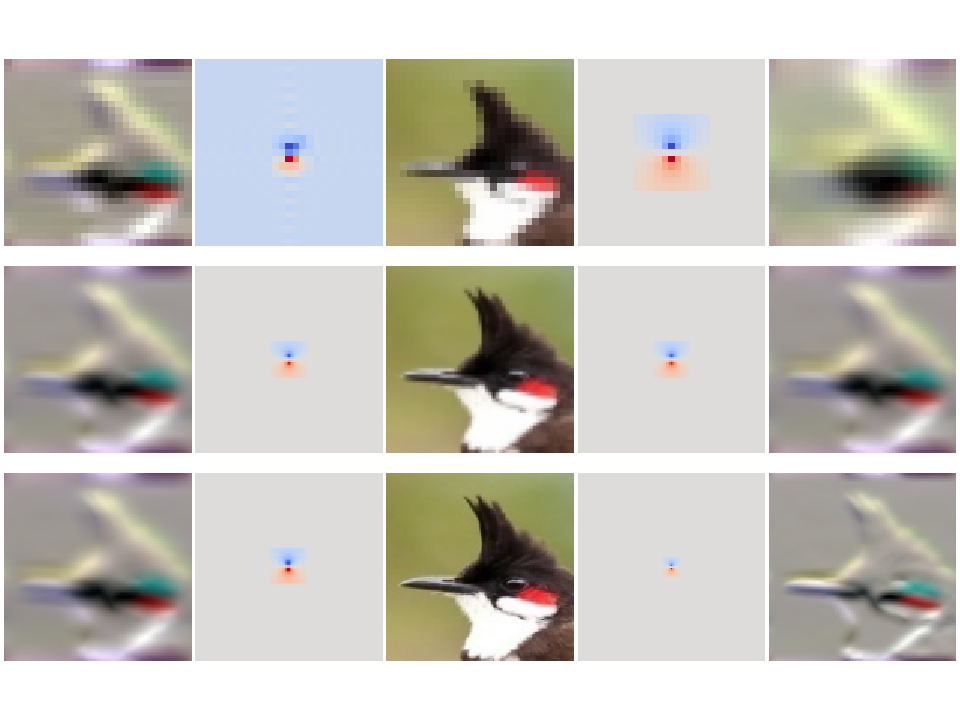
\includegraphics[width=\textwidth, trim= 0cm 1cm 0cm 1cm, clip]{atelier/FNO/res-conv-sobel.pdf}%
\end{minipage}%
\hfill%
\begin{minipage}{0.01\textwidth}
\phantom{-}
\end{minipage}
\end{minipage}
%}%
\hfill%
%
%
\begin{minipage}[t]{.5\textwidth}%
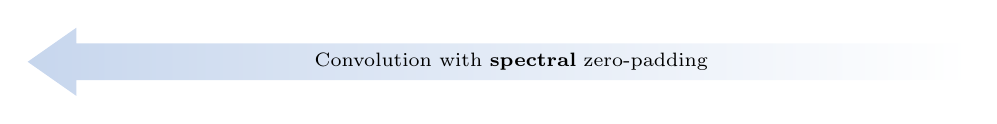
\begin{tikzpicture}[]
\node [
draw=none,
single arrow,
right color=white,
left color=fourierblue,
text=black,
single arrow head extend=0.2cm,
minimum height=\textwidth-5pt,
minimum width=.5cm,
single arrow tip angle=70,
shape border rotate=180
]{\scriptsize Convolution with 
\textbf{spectral} zero-padding};
\end{tikzpicture}\hfill%
%
\end{minipage}%
%
\begin{minipage}[t]{.5\textwidth}%
\hfill%
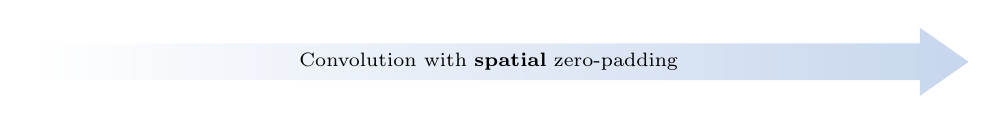
\begin{tikzpicture}[]
\node [
draw=none,
single arrow,
right color=fourierblue,
left color=white,
text=black,
single arrow head extend=0.2cm,
minimum height=\textwidth-5pt,
minimum width=.5cm,
single arrow tip angle=70,
shape border rotate=0
]{\scriptsize \phantom{-}Convolution with 
\textbf{spatial} zero-padding};
\end{tikzpicture}%
\end{minipage}%
\end{minipage}%
\caption[Effects of applying convolutional filters with different resolutions]{%
The image is taken from \cite[Fig. 1]{kabri2022FNO}---depicting a red whiskered bulbul taken from the Birds500 dataset \cite{pio450}---and visualize the different effects of spectral and spatial zero-padding.}
\label{fig:bulbul}
\end{figure}
%
%
We are given a kernel $\param\in\R^{\mathcal{J}_M}$, its unnormalized Fourier transform $\hat\param = \lambda F(\param)$ and an input $\imgg_N\in \R^{\mathcal{J}_N}$. If $M=N$, i.e. all dimension match, we observe that spectral and spatial implementation are equivalent, see the middle row of \cref{fig:bulbul}. However, if we consider higher resolution variant of the image with $N>M$, spatial zero-padding results in the kernel being localized in space and therefore the effect of convolving it with $\imgg_N$ changes. On the other hand for the spectral implementation we observe an equivariant behaviour. The resolution of the output changes but qualitatively the effect of the filter stay the same.
%
%
\paragraph{Connection to Interpolation}
%
As hinted in \cref{fig:bulbul}, when changing the resolution, the spectral implementation of convolution can be interpreted as a standard convolution with an interpolated kernel. In fact we observe that for $\param\in\R^{\mathcal{J}_M}, \hat\param=\lambda\, F(\param)$ and $\imgg_N\in\R^{\mathcal{J}_N}$ we have that
%
\begin{align*}
\CF(\hat\param)(\imgg_N) &= 
K(\hat{\param}^{M \rightarrow N})(\imgg_N) = 
F^{-1}\left(\hat{\theta}^{M \rightarrow N} \cdot Fv_N\right)\\ 
&= 
%
F^{-1}\left(F\, F^{-1}\hat{\theta}^{M \rightarrow N} \cdot Fv_N\right)\\
%
&=
F^{-1}\left(F \param^{M \xrightarrow{\Delta} N}  \cdot Fv_N \right)
%
=
%
\param^{M \xrightarrow{\Delta} N} \ast \imgg_N\\
%
&= 
C(\param^{M \xrightarrow{\Delta} N})(\imgg_N).
\end{align*}
%
%
Therefore, applying one FNO layer is equivalent to trigonometric interpolation of the kernel.
%
%
\paragraph{Adaption to Even Dimensions}
%
%
Zero-padding of the spectral coefficients only fulfills Hermitian symmetry in the case where $M,N$ are odd. In order ot adapt this to the even case, we employ so-called Nyquist splitting, see \cite{trigo19}. In all our experiments the implementation carefully employs this method, which ensures that the output of the spectral convolution is real valued.
%
%
\subsection{Analytical Results for FNOs}\label{sec:FNOAna}
%
%
In this section, we comment on the theoretical findings in \cite{kabri2023resolution}. We first consider the abstract neural layer as in \cref{eq:layerdef} for which we show continuity and Fréchet-differentiability.
%
%
\paragraph{Continuity of Neural Layers} The results for neural layers in \cite{kabri2023resolution} mostly fall back to the theory of \Nem{} operators, see e.g. \cite{tröltzsch, ambrosetti}. In order to show that the layer $\mathcal{G}$ is a well defined mapping from $L^p$ to $L^q$ one first needs to identify an exponent $r\in [1,\infty]$ such that the affine part is a mapping $\Psi:L^p\to L^r$. For example if $\kappa\in L^s$ with $1/r + 1 = 1/p + 1/s$ it follows from Young's convolution inequality that $\mathcal{K}$ maps to $L^r$, see \cite[Th. 1.2.12]{grafakos}. If then $W=0$ and $b\in L^r$ we know that $\Psi$ maps to $L^r$.

To ensure that the \Nem{} operator defines a mapping $\sigma:L^r\to L^q$ one needs to assume a growth condition on $\sigma:\R\to\R$, see \cite[Eq. 4]{kabri2023resolution} and originally \cite{tröltzsch}. Under these assumptions, we have the following result. The prove is trivial and the main content is buried in the assumptions, however it still summarizes the situation in a convenient way. Concrete examples fulfilling these assumptions are given in \cite{kabri2023resolution} borrowing concepts from \cite{ambrosetti, tröltzsch}. The most important activation function that is valid in this setting is the ReLU function
%
\begin{align*}
\relu(x) = \max\{x, 0\}.
\end{align*}
%
%
\begin{proposition}{\cite[Prop. 1]{kabri2023resolution}}{}
	For $1 \leq p, q \leq \infty$ let $\mathcal{L}$ be an operator layer given by \eqref{eq:layerdef} with an activation function $\sigma: \R \rightarrow \R$.
	If there exists $r \geq 1$ such that
	\begin{enumerate}[label=(\roman*)]
		\item the affine part defines a mapping $\Psi: L^p(\domain) \rightarrow L^r(\domain)$,
		\item the activation function $\sigma$ generates a Nemytskii operator $\sigma: L^r(\domain) \rightarrow L^q(\domain)$,
	\end{enumerate}
	%
	then it holds that
	%\begin{align*}
	$
	\mathcal{L}: L^p(\domain) \rightarrow L^q(\domain).
	$
	%\end{align*}
	If additionally $\Psi$ is a continuous operator on the specified spaces and the function $\sigma$ is continuous, or uniformly continuous in the case $q=\infty$, the operator $\mathcal{L}: L^p(\domain) \rightarrow L^q(\domain)$ is also continuous.
\end{proposition}
%
%
\paragraph{Differentiability of Neural Layers}
%
%
We furthermore consider Fréchet differentiability of a neural layer w.r.t. to the input variable. This can also be transferred to differentiability w.r.t. the parameters as we provide in \cite[Ex. 4]{kabri2023resolution}. Conceptually the main result we repeat here is similar to the one on continuity of the last paragraph. Namely, we put certain assumptions on the affine part and the activation function $\sigma:\R\to\R$ that allow us to employ the classical theory on \Nem{} operators. The major difference is that we also need to assume differentiability of the activation function, were we also assume a growth condition on the derivative. The ReLU function can therefore not be chosen in this setting, however the smooth approximation called GELU (\cite{hen16})
%
\begin{align*}
\operatorname{GELU}(x) := x\, \Phi(x)
\end{align*}
%
where $\Phi$ is the CDF of the standard normal distribution, can be employed.
%
%
\begin{proposition}{\cite[Prop. 2]{kabri2023resolution}}{}
	For $1 \leq p, q \leq \infty$, let $\mathcal{L}$ be an operator layer given by \eqref{eq:layerdef} with affine part $\Psi$ as in \eqref{eq:linearpart}. If there exists $r>q$, or $r = q = \infty$ such that
	\begin{enumerate}[label=(\roman*)]
		\item the affine part is a continuous operator $\Psi: L^p(\domain) \rightarrow L^r(\domain)$,
		\item the activation function $\sigma: \R \rightarrow \R$ is continuously differentiable
		\item and the derivative of the activation function generates a Nemytskii operator $\sigma': L^r(\domain) \rightarrow \left[L^r(\domain) \rightarrow L^{s}(\Omega) \right]$ with $s = {rq}/{(r-q)}$,
	\end{enumerate}
	then it holds that $\mathcal{L}:  L^p(\domain) \rightarrow L^q(\domain)$ is Fréchet-differentiable in any $v \in L^p(\domain)$ with Fréchet-derivative $D\mathcal{L}(v): L^p(\domain) \rightarrow L^q(\Omega)$
	\begin{align*}
		D\mathcal{L}(v)(h) = \sigma'(\Psi(v))\cdot\Tilde{\Psi}(h),
	\end{align*}
	where $\Tilde{\Psi}$ denotes the linear part of $\Psi$, i.e., $\Tilde{\Psi} = \Psi - b$.
\end{proposition}
%
%
\paragraph{Convertibility Between FNOs and CNNs}
%
%
The following lemma formalizes the intuition that FNOs and CNNs are equivalent in certain settings. Given inputs of a fixed discretization $\mathcal{J}_N$ and parameters $\param\in\R^{\mathcal{J}_M}$ the standard convolution implementation is equivalent to the spectral one w.r.t. the parameters $\hat\param = \lambda\, F(\param^{M\to N})$. The subtle but important point here, is that the number of spectral parameters needs to be equal to the input size in order to achieve equivalence. In \cite[Fig.3]{kabri2023resolution} we observe numerically that the number of used spectral coefficients actually needs to match the input size in order to achieve equivalence.
%
%
\begin{lemma}{\cite[Lem. 3]{kabri2023resolution}}{lem:FNOconv}
	Let $M \leq N$ both be odd and let $T: \R^{J_N} \rightarrow \mathbb{C}^{I_N}$ be defined for $\theta \in \R^{J_N}$ as
	$T(\theta) = \lambda \, F(\theta)$.
	For any $\theta \in \R^{J_M}$ and $v \in \R^{J_N}$ it holds true that
	\begin{align*}
		C(\theta)(v) = K(T(\theta^{M\rightarrow N}))(v)
	\end{align*}
	and for any $\hat{\theta} \in \mathbb{C}^{I_M}_{\text{sym}}$ and $v \in \R^{J_N}$ it holds true that
	\begin{align*}
		K(\hat{\theta})(v) = C(T^{-1}(\hat{\theta}^{M\rightarrow N}))(v).
	\end{align*}
\end{lemma}
%
%
\noindent%
From this and from \cite[Fig. 3]{kabri2023resolution} we obtain the negative result that in order to convert a CNN to a FNO we need a large number of spectral parameters. This also connected to the fact that spatial locality can usually only expressed using more spectral coefficients. Therefore, one might think that FNOs are infeasible due to memory requirements. However, it turns out that directly optimizing over the spectral parameters leads to a comparable performance, already for a low number of Fourier coefficients. This is reported in the blue curve in \cite[Fig. 3]{kabri2023resolution}. This hints, that while the forward pass can be equivalent, computing the gradient w.r.t. their parameters is not. This is formalized in the following lemma.
%
%
\begin{lemma}{\cite[Lem. 4]{kabri2023resolution}}{lem:FNOGrad}
For odd $N \in \mathbb{N}$ and $v, \theta \in \R^{J_N}$ and $\hat{\theta} = T(\theta)$ it holds true that
\begin{align*}
	\nabla_{\hat{\theta}} K(\hat{\theta})(v) = \frac{1}{|J_N|}\; T \left( \vphantom{\hat{\theta}} \nabla_{\theta}C(\theta)(v) \right). 
\end{align*}
\end{lemma}
%
%
\paragraph{Interpolation Equivariance}
%
%
The last result considers the main motivation for the topic. Namely, the resolution in-variance of an FNO layer. However, here we can not allow an arbitrary resizing operation. Since it is most natural to our approach, we can show equivariance w.r.t. trigonometric interpolation of the input.
%
%
\begin{corollary}{}{cor:FNOequi}
	For $\hat{\theta} \in \mathbb{C}^{I_M}_{\text{sym}}$, $v \in \R^{J_N}, M \leq N$ it holds true for any $L \geq M$ that
	\begin{align*}
		K(\hat{\theta})(v^{N \xrightarrow{\Delta} L}) = \left( K(\hat{\theta})(v) \right)^{N \xrightarrow{\Delta} L}.
	\end{align*}
\end{corollary}


\subsection{Numerical Results}\label{sec:FNONum}
%
%
\begin{wrapfigure}{r}{.4\textwidth}
\begin{center}
	
\includegraphics[width=.4\textwidth]{atelier/FNO/FNOQR.png}
\end{center}
The code for all the experiments is available at \href{https://github.com/samirak98/FourierImaging}{https://github.com/samirak98/}\\
\href{https://github.com/samirak98/FourierImaging}{FourierImaging}.
\end{wrapfigure}
%
%
In the numerical section of \cite{kabri2023resolution} we study the convertibility of CNNs to FNOs as discussed in \cref{sec:FNOAna} and the resolution invariance of the different proposed approaches. Again we employ---among others---the \texttt{PyTorch} package \cite{paszke2019pytorch}. The experiments are conducted on the FashionMNIST \cite{Han17} and a former version of the BIRDS500 \cite{pio450} dataset. We remark that our implementation carefully treats the case of even kernel or input sizes, via Nyquist splitting. This allows us to apply all the derived results for the odd and also the even case.
%
%
\paragraph{Convertibility and Training Differences} As already described in \cref{sec:FNOAna} the first experiment, displayed in \cite[Fig. 3]{kabri2023resolution}, studies how CNNs can be converted to FNOs. Here, we employ a network with two convolutional layers for feature extraction and a linear classification layer. We train this network---in the spatial implementation---on the FashionMNIST dataset employing varying spatial kernel sizes. Here, we see that for $M=5$ the spatial implementation already has the best performance and adding more parameters does not increase the performance. We then convert a set of spatial parameters to the Fourier formulation, employing again a varying number of spectral coefficients. It turns out that the requirement of \cite[Lem. 3]{kabri2023resolution}, that the number of coefficients must match the input dimension is indeed relevant. We only obtain the full performance of the CNN if we use all spectral parameters. However, the example also visualizes \cite[Lem. 4]{kabri2023resolution}, namely that training a FNO conceptually leads to a different set of parameters. Optimizing over the spectral parameters yields a comparable performance already for a smaller number of coefficients.
%
%
\paragraph{Resolution Invariance}
%
In the second experiment we study the resolution invariance of the three discretization independent architectures we considered, namely the naive CNN adaptation, input interpolation and the FNO implementation. We first train the convolutional architecture as in the previous paragraph on the FashionMNIST dataset, that has an input size of $28\times 28$. We resize the input data via trigonometric and bilienear interpolation---referred to as data sizing---to simulate multi-resolution data. One expects that the classification performance drops when the data is resized to a smaller size, since this step looses information. However, resizing the images to higher resolutions should yield the same performance.

In \cite[Fig. 4]{kabri2023resolution} see that the simple adaption does not perform well both in the lower and the higher resolution setting. Employing input interpolation improves the performance in the lower resolution setting. In the higher resolution regime, we obtain a constant performance which is expected. Finally we see that the FNO---which was converted from the CNN---performs as well as input interpolation, which justifies the resolution independence of this architecture.

In the second experiments we trained a ResNet18 \cite{he2016deep} on a former version of the BIRDS500 dataset, with an input size of $112\times 112$. Concerning the naive adaption and the input interpolation we observe the same behavior as in the previous example. However, the FNO variant performs slightly worse, which is surprising, especially in the higher resolution regime. In \cite{kabri2023resolution} we conclude that this is due the dimension changes within the ResNet architectures. These changes occur due to strided convolutions or pooling operations between the layers. In fact in order to achieve the performance as displayed in \cite[Fig. 4 (b)]{kabri2023resolution} we replaced every striding by a trigonometric interpolation, which fits better into the FNO framework and vastly improves the performance. Therefore, we summarize that architecture intern dimension changes---which are very common in practice---can potentially hinder resolution invariance.
\chapter{Conclusion}\label{ch:C}
%
%
This thesis provided insights in the topics of consistency, sparsity and robustness of learning algorithms. Thematically, the thesis is split into two main chapters, dealing with semi-supervised and supervised learning. We summarize both chapters below and respectively provide an outlook and possible future work.

\paragraph{Consistency of SSL on Sparse Graphs} We considered the infinite data limit in the semi-supervised setting, focusing on the Lipschitz learning task. For all our results we assumed a mild scaling conditions which allow for very sparse graphs. We were first able to show $\Gamma$-convergence in the variational setting. We then proved convergence rates for AMLEs via a homogenization strategy, where we the proof relied on the comparison with cones principle. The key insight we obtained was, that a rate for graph distance functions implies a rate for graph AMLEs. This observation was already employed in our follow-up work in \cite{bungert2022ratio}, where convergence rate at a even smaller scale was shown. We also conducted experiments to validate our theoretical framework in practice. Here, we observed better results than we were able to prove. 

While our framework allows the graph to be very sparse, we are restricted to the case of ball graphs. Here it would be interesting to see, how our results can be transferred to the knn setting as in \cite{calder2022improved}. Furthermore, we only considered the standard Lipschitz learning task, that tends to forget the data distribution, which is undesirable for many learning tasks. In \cite{calder2019consistency} a modification was proposed that makes the problem sensitive to the distribution. The open problem that arises here, is how to adapt the technique in \cite{bungert2021uniform} to show convergence for the modified problem.\par

\paragraph{Robust and Sparse SL} In the supervised setting, we considered input-robustness w.r.t. adversarial perturbations and resolution changes. In the first case we proposed a defense mechanism to train stable neural networks, based on Lipschitz regularization. We provided analytical results and numerical experiments which suggest that the strategy allows to learn robust networks. The strength of this approach depends on how well the discrete Lipschitz constant approximates the true one. An interesting future direction would be to explore different methods to determine the discrete set of Lipschitz pairs. E.g. one could additionally learn a generative model that outputs these pair in a faster and probably even more expressive way than the gradient descent scheme, employed right now.

For the multi-resolution setting we analyzed the role of Fourier neural operators. We first showed functional analytic properties of neural layers acting on $L^p$ spaces. We then established the relation of disctretized Fourier layers to standard convolution operations, both from a theoretical and a practical side. We also highlighted the importance of the trigonometric interpolation in this context. We conducted numerical tests that suggest the resolution equivariant behavior of FNO layers. Connected to the previous topic it would be interesting to study the adversarial robustness of FNOs. First numerical tests in \cite{kabri2022FNO} hint that the vulnerabilities are even worse than in the standard case.

We considered the question on how to enforce sparsity in neural network weights. Here, we employed a stochastic variant of Bregman iterations, which allowed to train networks that are very sparse throughout the whole optimization. We provided theoretic convergence guarantees, where the main novelty was the stochasticity introduced into the iteration. We also showed the numerical efficiency of the method, by training sparse neural networks performing similarly to their dense counterparts. One open problem is to weaken the convexity assumption and instead prove the convergence result, by employing a Kurdyka–\L{}ojasiewicz type inequality as in \cite{benning2018choose}. Concerning the neural architecture search via sparsity as proposed in our work, a further interesting task would be to learn the U-Net type architecture of \cite{ronneberger2015u}.

\printbibheading
\printbibliography[type = book,
                   title = Books,
                   heading = subbibliography]
\printbibliography[type = article,
                   title = Articles,
                   heading = subbibliography]
\printbibliography[type = thesis,
				   title = Theses,
				   heading = subbibliography]
\printbibliography[type = online,
                   title = Online,
                   heading = subbibliography]
%%-------------------------------------------------
\part{Prints}\label{part:Prints}
\renewcommand{\expprefix}{P}
\setcounter{chapter}{0}
\renewcommand{\chapapp}{Print}
\paperchapter{roith2022continuum}{}{}{1}{1}
\paperchapter{bungert2021uniform}{}{}{1}{1}
%% %
\paperchapter{bungert2021clip}{}{}{1}{0}
\paperchapter{bungert2022bregman}{}{}{1}{1}
\paperchapter{kabri2023resolution}{}{}{1}{0}
%-------------------------------------------------
%\declarationGer
%-------------------------------------------------
\end{document}
